\documentclass[10pt,a4paper]{article}

\usepackage[a4paper,margin=17mm]{geometry}
\usepackage[T1]{fontenc}
\usepackage[utf8]{inputenc}
\usepackage{microtype}
\usepackage{amsmath,amssymb,bm}
\usepackage{array,booktabs,longtable,tabularx}
\usepackage{graphicx}
\usepackage{xcolor}
\usepackage{siunitx}
\usepackage{caption}
\usepackage{subcaption}
\usepackage{float}
\usepackage[numbers,sort&compress]{natbib}
\usepackage{xurl}
\usepackage[hidelinks]{hyperref}
\usepackage{enumitem}

\sisetup{per-mode=symbol, exponent-product=\cdot}
\setlength{\parindent}{0pt}
\setlength{\parskip}{0.45em}
\setlength{\tabcolsep}{3.5pt}
\renewcommand{\arraystretch}{1.12}
\sloppy
\hbadness=10000
\setlist[itemize]{leftmargin=1.3em,itemsep=0.15em,topsep=0.2em}
\setlist[enumerate]{leftmargin=1.5em,itemsep=0.15em,topsep=0.2em}

\newcommand{\code}[1]{\texttt{\detokenize{#1}}}
\newcommand{\uu}{\bm{u}}
\newcommand{\sig}{\bm{\sigma}}
\newcommand{\I}{\bm{I}}
\newcommand{\grad}{\nabla}
\newcommand{\divv}{\nabla\!\cdot}
\newcommand{\TT}{T}
\newcommand{\pp}{p_\ell}
\newcommand{\pcap}{p_c}
\newcommand{\rhoW}{\rho_\ell}
\newcommand{\muW}{\mu_\ell}
\newcommand{\npor}{n}
\newcommand{\Sat}{S_\ell}
\newcommand{\alphaB}{\alpha_B}
\newcommand{\vW}{\bm v_\ell}
\newcommand{\K}{\bm K}
\newcommand{\krel}{k_{\mathrm{rel}}}
\newcommand{\thetaw}{\theta}
\newcommand{\Oop}{\mathcal O}
\newcolumntype{Y}{>{\raggedright\arraybackslash}p{0.34\textwidth}}
\newcolumntype{L}[1]{>{\raggedright\arraybackslash}p{#1}}

\title{\textbf{CD-A OGS TRM Model and Measurement-Data Technical Report}\\
\large PDE model, OGS implementation, stochastic inputs, heterogeneity feasibility, and evidence annex}
\author{Prepared from the CD-A model, measurement catalogue, and generated audit outputs}
\date{Generated 2026-06-01}

\begin{document}
\maketitle

\begin{abstract}
This report is a standalone technical synthesis for the CD-A Niche 4 OpenGeoSys
(OGS) Thermo--Richards--Mechanics (TRM) model and the currently available
measurement data.  It states the governing equations, maps the OGS XML quantities
to fields, units, and stochastic input choices, and evaluates which parameters or
materials are technically defensible candidates for heterogeneity.  It also records
how each measurement class enters the model: as an active likelihood term, a
diagnostic observation operator, a boundary-condition audit, a support/prior layer,
or a not-yet-ready hard residual.  The final annex consolidates the main findings
from the previous data-mining and inversion audits, including figures and scenario
consequences.  No access to local folders is required to understand the modelling
state described here.
\end{abstract}

\section*{Current Technical Position}

The exchanged CD-A OGS model is a frozen two-dimensional TRM model for liquid
pressure, temperature, and displacement.  The only material field currently released
as an active inversion unknown is the intrinsic permeability tensor field
\(\K(\bm x)\), introduced through OGS \code{MeshElement} cell data without changing
the process equations.  Porosity is present as a mesh field but remains fixed at
\(\npor=0.105\); retention, elasticity, swelling, thermal constants, and boundary
curves are not active material unknowns in the present objective.

The current active objective has two measurement contributors: 75 direct
permeability pulse-test rows and 192 sampled NMR water-content rows.  The current
packaged field is accepted as the active-objective incumbent, with objective
3156.353, direct permeability component 269.818, and raw-NMR state component
2886.535.  It is not a final all-measurement field.  ERT, Taupe/TDR, RH/suction,
other-HM monitoring, historical endpoint rows, and the suspicious thermal-expansion
\code{CTE} value remain gated by missing provider information or internal modelling
decisions \citep{GeneratedAuditSuite2026}.

\tableofcontents
\clearpage

\part*{Part I -- PDE Model, OGS Implementation, and Data Ties}
\addcontentsline{toc}{part}{Part I -- PDE Model, OGS Implementation, and Data Ties}

\section{Model Scope and State Variables}

The model is the OGS \code{THERMO_RICHARDS_MECHANICS} process, using the same
mathematical structure as the TRM formulation documented by OGS and closely related
to the coupled THM notation of \citet{Wang2009THM}.  Vapor diffusion is not active;
gas pressure is treated implicitly through the Richards capillary-pressure
convention.  Gravity is disabled in the recovered process settings.  The primary
unknowns are:

\begin{longtable}{@{}L{0.18\textwidth}L{0.18\textwidth}L{0.16\textwidth}Y@{}}
\caption{Primary and derived fields used in the CD-A OGS TRM model.}\\
\toprule
Field & Symbol & Unit & Role in model and data comparison \\
\midrule
\endfirsthead
\toprule
Field & Symbol & Unit & Role in model and data comparison \\
\midrule
\endhead
\bottomrule
\endlastfoot
Liquid pressure & \(\pp\) & Pa & Primary hydraulic variable.  Appears in storage, Darcy flow, capillary pressure \(p_c=-p_\ell\), and Bishop pore-stress coupling.  RH/suction data audit or reconstruct pressure boundary curves. \\
Temperature & \(\TT\) & K & Primary thermal variable.  Current runs are nearly isothermal at 298.15 K, so thermal parameters are fixed and weakly identifiable. \\
Displacement & \(\uu\) & m & Primary mechanical variable.  HM monitoring could constrain it, but numeric exports are not currently available for hard residuals. \\
Liquid saturation & \(\Sat\) & -- & OGS secondary state from the van Genuchten retention law.  NMR, ERT, Taupe/TDR, and RH all relate to it indirectly. \\
Volumetric water-content proxy & \(\thetaw=\npor\Sat\) & -- or fraction & Model-side water-content proxy sampled from OGS.  It is not equal to total NMR water in clay without a bound/interlayer-water term. \\
Intrinsic permeability tensor & \(\K(\bm x)\) & \(\mathrm{m^2}\) & Active heterogeneous material field.  Direct pulse tests constrain interval-scale projections of \(\K\). \\
Darcy velocity & \(\vW\) & \(\mathrm{m\,s^{-1}}\) & Derived from \(\K\), \(\krel(\Sat)\), viscosity, and pressure gradient; controls hydraulic evolution and advective heat term. \\
Stress and strain & \(\sig,\bm\varepsilon\) & Pa, -- & Mechanical response through orthotropic elasticity, Bishop stress, thermal strain, and swelling strain. \\
\end{longtable}

\section{Governing Equations}

\subsection{Darcy Flow}

The liquid Darcy velocity in the configured model is
\[
  \vW = -\frac{\krel(\Sat)\,\K}{\muW}\grad \pp ,
  \qquad
  \bm q_\ell=\rhoW\vW .
\]
The specific body force is zero in the model, so no gravity term enters the Darcy
law.  The factors \(\npor\Sat\) are storage and thermal-mixing terms; they are not
part of the Darcy velocity.  The permeability tensor \(\K\) is intrinsic
permeability in \(\mathrm{m^2}\), while liquid mobility is
\(\krel\K/\muW\) \citep{OpenGeoSysTRMDocs}.

\subsection{Liquid Mass Balance}

For the no-vapor TRM case the hydraulic equation can be written as
\[
\left(\Sat\beta-\npor\frac{\partial\Sat}{\partial \pcap}\right)\rhoW\dot{\pp}
-
\Sat\left(\frac{\partial\rhoW}{\partial\TT}
      +\rhoW(\alphaB-\Sat)\alpha_T^s\right)\dot{\TT}
+ \divv(\rhoW\vW)
+ \Sat\alphaB\rhoW\divv\dot{\uu}
= Q_H,
\qquad
\pcap=-\pp .
\]
The OGS liquid density is not constant:
\[
\rhoW(\TT,\pp)
=1095\left[1-5\times10^{-4}(\TT-298.15)
+3.2\times10^{-10}(\pp-7.5\times10^6)\right].
\]
Thus both pressure and temperature derivatives contribute to storage/coupling.  The
active inversion mostly identifies \(\K\) through its control on \(\vW\), saturation,
and desaturation timing.  Retention parameters and boundary pressure can mimic
permeability changes, so they remain gated until RH and NMR semantics are settled.

\subsection{Momentum Balance}

The quasi-static mechanical balance is
\[
\divv\left(\sig - b(\Sat)\alphaB \pp\,\I\right)+\bm f = \bm 0,
\qquad
\sig = \bm C:\left(\bm\varepsilon(\uu)-\bm\varepsilon^T
-\bm\varepsilon^{\mathrm{sw}}(\Sat)\right).
\]
Here \(\bm f=\bm{0}\), \(\alphaB=1\), and the configured Bishop law has exponent
one, so \(b(\Sat)=\Sat\).  Orthotropic elasticity is active.  Saturation-dependent
swelling is also active, but no numeric deformation time-series is currently
available to calibrate swelling or elasticity.  They are retained as fixed model
structure, with later validation possible if Geoscope, levelling, crackmeter, or
laser-scan numeric exports become available \citep{Amann2015}.

\subsection{Heat Balance}

The heat equation is
\[
(\rho c_p)^{\mathrm{eff}}\dot{\TT}
-\divv\left(\bm k_T^{\mathrm{eff}}\grad \TT\right)
+\rhoW c_w\,\grad \TT\cdot\vW
=Q_T,
\]
with OGS effective phase mixing
\[
(\rho c_p)^{\mathrm{eff}}=(1-\npor)\rho_s c_s+\npor\Sat\rhoW c_w,
\qquad
\bm k_T^{\mathrm{eff}}=(1-\npor)\bm k_T^s+\npor\Sat k_T^\ell\I .
\]
The CD-A data collected for this workflow are dominated by hydraulic, water-content,
geophysical, and HM monitoring streams.  There is no active thermal-gradient
likelihood.  Therefore thermal conductivity, heat capacities, liquid viscosity, and
liquid density slopes are treated as fixed in the current report.

\subsection{Domain and Boundary Conditions}

\begin{figure}[H]
\centering
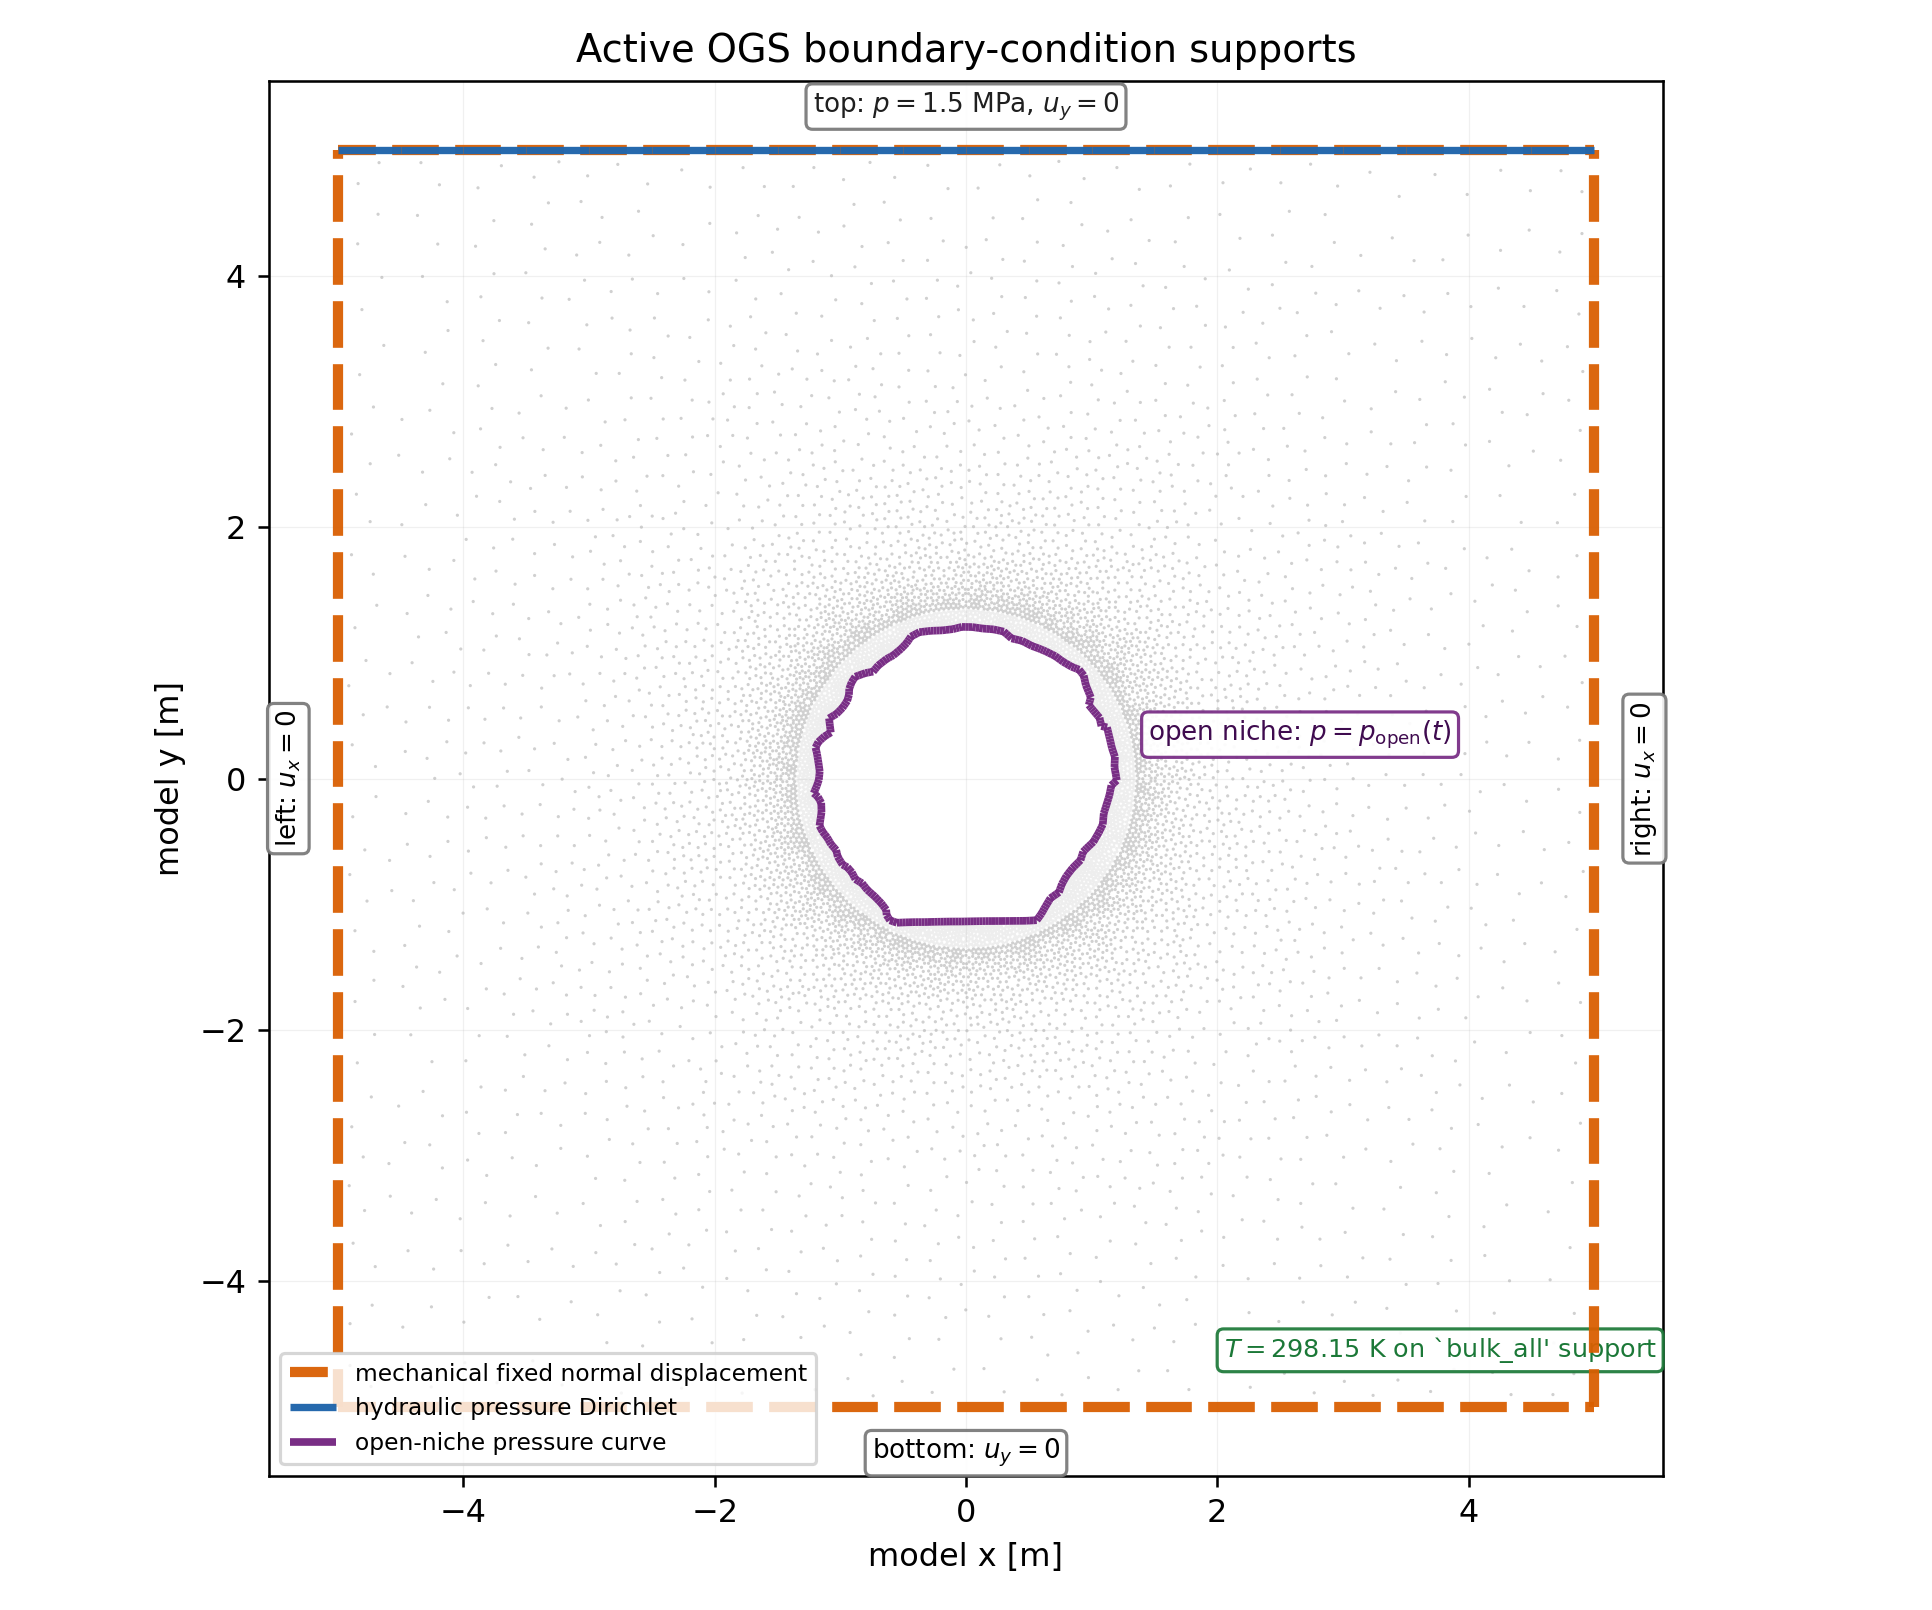
\includegraphics[width=0.86\textwidth]{figures/boundary_conditions_domain.png}
\caption{Active boundary-condition supports in the current OGS model.  The orange
dashed outer box is the mechanical fixed-normal-displacement support.  The blue top
edge is the constant hydraulic pressure support, and the purple niche wall is the
time-dependent open-niche pressure support.  Temperature is fixed at 298.15 K on the
\code{bulk_all} support, which keeps the current model effectively isothermal.}
\label{fig:boundary-conditions}
\end{figure}

\begin{longtable}{@{}L{0.17\textwidth}L{0.17\textwidth}L{0.26\textwidth}Y@{}}
\caption{Active initial and boundary conditions used by the TRM model.}\\
\toprule
Process part & Initial state & Active boundary support & Modelling consequence \\
\midrule
\endfirsthead
\toprule
Process part & Initial state & Active boundary support & Modelling consequence \\
\midrule
\endhead
\bottomrule
\endlastfoot
Hydraulic pressure \(\pp\) & \(\code{ic_pressure}\), a function that evaluates to 1.5 MPa in the recovered settings. & \(\code{cd-a_top}\): Dirichlet \(\code{bc_top_pressure}=1.5\) MPa.  \(\code{cd-a_niche4}\): Dirichlet \(\code{open_niche_seasonal}\), a \(\code{CurveScaled}\) pressure curve with scaling factor 1.0.  Other pressure boundaries have no explicit pressure condition and therefore use the natural no-flow condition. & The open-niche curve is the dominant desaturation forcing.  In the active curve file it spans about \(-5.23\) to \(-53.24\) MPa over roughly \(1.35\times10^8\) s.  RH/suction data audit this forcing, but the source curve provenance and sensor-screening policy are still open. \\
Temperature \(\TT\) & \(\code{ic_temperature}=298.15\) K. & \(\code{bulk_all}\): Dirichlet \(\code{bc_temperature_outside}=298.15\) K. & The recovered support is domain-wide rather than a calibrated thermal loading boundary, so the current runs are effectively isothermal.  Thermal parameters remain fixed and are not released by the present likelihood. \\
Mechanical displacement \(\uu\) & Zero initial displacement, \(\uu=(0,0)\). & Left/right boundaries: Dirichlet component 0, \(u_x=0\).  Top/bottom boundaries: Dirichlet component 1, \(u_y=0\). & This is a roller-type outer-box constraint for the 2D mechanical problem.  It defines the displacement support for HM validation, but no numeric HM time series are ready for hard residuals. \\
Mechanical loads and stress bookkeeping & Body force is \(\bm{0}\).  A parameter \(\code{ic_sigma0}\) exists, but the process line \(\code{initial_stress}\) is commented out. & A top Neumann load \(\code{load_top}\) is present only in a commented boundary-condition block. & These definitions are not active calibration inputs in the current OGS run.  They should remain provenance notes unless the process-variable XML is changed and rerun. \\
Inactive pressure alternatives & None active. & \(\code{bc_pressure_outside}\), \(\code{bc_atm_pressure}\), and \(\code{closed_niche_seasonal}\) are defined or retained as commented/source alternatives, but are not referenced by the active pressure process variable. & They should not be interpreted as fitted boundary conditions.  The current report concerns the open-niche \(\code{cd-a_niche4}\) pressure curve. \\
\end{longtable}

\section{Constitutive Laws and Fixed Values}

\begin{longtable}{@{}L{0.23\textwidth}L{0.13\textwidth}L{0.14\textwidth}Y@{}}
\caption{Configured material, fluid, and coupling parameters.}\\
\toprule
Quantity & Symbol & Unit & Value, model, or current decision \\
\midrule
\endfirsthead
\toprule
Quantity & Symbol & Unit & Value, model, or current decision \\
\midrule
\endhead
\bottomrule
\endlastfoot
Porosity & \(\npor\) & -- & Fixed support field, \(\npor=0.105\).  It enters storage, thermal mixing, and \(\thetaw=\npor\Sat\). \\
Intrinsic permeability & \(\K\) & \(\mathrm{m^2}\) & Base tensor \(\mathrm{diag}(1.00\times10^{-19},4.00\times10^{-20})\).  Active field uses OGS cell data \(\code{k_i_rd}\). \\
Biot coefficient & \(\alphaB\) & -- & Fixed at 1.0. \\
Liquid viscosity & \(\muW\) & Pa s & Fixed \(1.0\times10^{-3}\). \\
Liquid density & \(\rhoW\) & \(\mathrm{kg\,m^{-3}}\) & Linear law above; reference 1095 at \(298.15\) K and \(7.5\) MPa. \\
Solid density & \(\rho_s\) & \(\mathrm{kg\,m^{-3}}\) & Fixed \(2.52\times10^3\). \\
Solid heat capacity & \(c_s\) & \(\mathrm{J\,kg^{-1}\,K^{-1}}\) & Fixed 1254.74. \\
Liquid heat capacity & \(c_w\) & \(\mathrm{J\,kg^{-1}\,K^{-1}}\) & Fixed 4160. \\
Solid thermal conductivity & \(k_s\) & \(\mathrm{W\,m^{-1}\,K^{-1}}\) & Fixed 2.156. \\
Liquid thermal conductivity & \(k_\ell\) & \(\mathrm{W\,m^{-1}\,K^{-1}}\) & Fixed 0.6. \\
Thermal expansivity & \(\alpha_T^s\) & \(\mathrm{K^{-1}}\) & XML value is 1254.74 and is not physically plausible for rock thermal expansion.  It is a provenance blocker, not a calibrated property. \\
Elasticity & \(\bm C\) & Pa & Orthotropic linear elasticity: \(E_1=13.8\) GPa, \(E_2=6.0\) GPa, \(E_3=13.8\) GPa; \(G_1=4.79\) GPa, \(G_2=2.46\) GPa, \(G_3=4.79\) GPa; \(\nu_{12}=0.44\), \(\nu_{23}=0.22\), \(\nu_{13}=0.44\). \\
Swelling & \(\bm\varepsilon^{\mathrm{sw}}\) & -- & OGS saturation-dependent swelling; swelling pressures \(1.0\) MPa in each principal direction, exponents 1, active over \(S\in[0.1,1]\). \\
Bishop function & \(b(\Sat)\) & -- & \(b(\Sat)=\Sat\). \\
Retention curve & \(\Sat(\pcap)\) & -- & van Genuchten drying curve with \(S_{\ell r}=0.1\), \(S_{gr}=0\), \(m=0.45\), \(p_b=10\) MPa. \\
Relative permeability & \(\krel(\Sat)\) & -- & van Genuchten--Mualem with \(S_{\ell r}=0.1\), \(S_{gr}=0\), \(m=0.45\), and \(k_{\mathrm{rel}}^{\min}=10^{-25}\) \citep{VanGenuchten1980}. \\
\end{longtable}

The configured saturation law is
\[
\Sat(\pcap)=S_{\ell r}+(1-S_{\ell r}-S_{gr})
\left[1+\left(\frac{\pcap}{p_b}\right)^{1/(1-m)}\right]^{-m}.
\]
The corresponding relative permeability is
\[
S_e=\frac{\Sat-S_{\ell r}}{1-S_{\ell r}-S_{gr}}, \qquad
\krel(\Sat)=S_e^{1/2}\left[1-\left(1-S_e^{1/m}\right)^m\right]^2,
\]
subject to the configured numerical floor.

\section{Stochastic Inputs and Prior Ranges}

The staged Bayesian interpretation should release only parameters that the current
data can identify.  Table~\ref{tab:stochastic} separates active stochastic fields
from later-release candidates and blocked provenance items.

\begin{longtable}{@{}L{0.21\textwidth}L{0.2\textwidth}L{0.2\textwidth}Y@{}}
\caption{Candidate stochastic inputs and defensible prior ranges.}
\label{tab:stochastic}\\
\toprule
Input & Current value & Candidate stochastic model & Current release decision \\
\midrule
\endfirsthead
\toprule
Input & Current value & Candidate stochastic model & Current release decision \\
\midrule
\endhead
\bottomrule
\endlastfoot
Permeability magnitude field \(k_{\mathrm{mag}}(\bm x)\) & Geometric reference \(6.32\times10^{-20}\,\mathrm{m^2}\) & Lognormal random field:
\(\ln k_{\mathrm{mag}}\sim\mathcal N(\ln(6.32\times10^{-20}),0.5^2)\), then conditioned/updated by pulse tests.  Local support lengths tested from about 0.003 to 0.075 m; current accepted local-basis field uses a short deterministic support around 30 anchor cells. & Active stage-1 unknown.  Strongest data support. \\
Permeability anisotropy ratio \(r=k_\parallel/k_\perp\) & 2.5 & \(\ln r\sim\mathcal N(\ln 2.5,0.4^2)\), if released. & Keep fixed for current stage.  Global and local anisotropy screens did not justify release from current data. \\
Permeability orientation \(\theta_K\) & Bedding-informed \(144^\circ\) & \(\theta_K\sim\mathcal N(144^\circ,(15^\circ)^2)\), if released. & Keep global orientation fixed unless support/likelihood and directional evidence improve. \\
Porosity \(\npor\) & 0.105 & Possible scalar \(\mathcal N(0.105,0.02^2)\), bounded to physically plausible OPA range. & Fixed support.  NMR cannot separate porosity, saturation, and bound/interlayer water alone. \\
van Genuchten \(p_b\) & 10 MPa & \(p_b\sim\mathcal U(5,20)\) MPa. & Later scalar candidate only after RH boundary provenance and state residual policy close. \\
van Genuchten exponent \(m\) & 0.45 & \(m\sim\mathcal N(0.45,0.05^2)\), clipped to plausible retention-shape values. & Later scalar candidate; strongly correlated with \(p_b\), boundary pressure, and porosity. \\
Residual saturations & \(S_{\ell r}=0.1\), \(S_{gr}=0\) & No current stochastic release. & Fixed until independent retention/hysteresis evidence is available. \\
Open-niche pressure curve & Existing model curve & Possible documented curve family from RH sensor policies after provenance confirmation. & Blocked; not a material property and not safe to fit blindly. \\
Elasticity, Biot, swelling & Fixed orthotropic/swelling parameters & Later validation or mechanical calibration only if numeric HM time series are obtained. & Fixed.  Current data do not identify them. \\
Thermal constants and CTE & Fixed XML values; CTE suspicious & No stochastic release. & CTE needs provenance confirmation; thermal constants are unsupported by current data. \\
\end{longtable}

\section{Feasibility of Heterogeneous Materials}

The host rock and experiment support heterogeneity in principle.  The CD-A niches are
in bedded Opalinus Clay with EDZ development, structural/facies variation, faults or
fractures, and strong scale dependence of hydraulic/geophysical measurements
\citep{Ziefle2021Sand,Ziefle2024Characterization,WaterContentEDZ2024}.  The
modelling question is narrower: which heterogeneous fields are identifiable from the
available measurements without absorbing boundary-condition or observation-operator
errors?

\begin{longtable}{@{}L{0.19\textwidth}L{0.18\textwidth}L{0.19\textwidth}Y@{}}
\caption{Feasibility of treating candidate materials/fields as heterogeneous.}\\
\toprule
Field or material & Physical plausibility & Data identifiability & Recommendation and expected effect on model evolution \\
\midrule
\endfirsthead
\toprule
Field or material & Physical plausibility & Data identifiability & Recommendation and expected effect on model evolution \\
\midrule
\endhead
\bottomrule
\endlastfoot
Intrinsic permeability magnitude \(\K(\bm x)\) & High.  EDZ, bedding, faults, desaturation damage, and pulse-test spread all support local variability. & Moderate to high for local intervals: 75 active pulse-test rows, 52 duplicate-aware groups, but only around BCD-A32/A33 in current mesh. & Treat as heterogeneous now.  It strongly affects pressure diffusion, desaturation timing, \(\thetaw\), ERT/Taupe trends, and HM response.  Do not call the field final while diagnostic streams remain gated. \\
Permeability tensor orientation/anisotropy & High as a bedding-controlled effect. & Low to moderate.  Direct pulse tests are scalar interval observations; local/global anisotropy screens did not improve the current objective. & Keep fixed at bedding-informed angle and 2.5 ratio for now.  Releasing tensor shape can overfit support errors and would affect lateral redistribution more than local magnitude updates. \\
EDZ/fault-zone permeability classes & High.  The experiment is explicitly about EDZ evolution and niche contrasts. & Potentially useful, but current active data are sparse and support-conflicted; ERT/Taupe could help if calibrated. & Feasible as a later structured field family.  Prefer structural priors over unconstrained cell-wise noise. \\
Porosity \(\npor(\bm x)\) & Plausible due to damage, facies, and water-loss porosity variation. & Currently weak.  NMR measures total hydrogen-bearing water and is confounded by saturation and bound/interlayer water. ERT/Taupe calibration is open. & Keep fixed.  Heterogeneous porosity would directly change \(\thetaw=\npor\Sat\), storage, and thermal mixing, so release only after NMR/RH/ERT/Taupe semantics are settled. \\
Retention parameters \(p_b,m,S_{\ell r}\) & Plausible facies/stress variation. & Weak at present.  RH is boundary/provenance audit only; NMR/ERT/Taupe state data are gated. & Keep scalar/fixed.  Heterogeneous retention would strongly affect desaturation fronts and can mimic permeability or boundary-pressure changes. \\
Elastic stiffness and Biot coefficient & Plausible anisotropic and scale-dependent OPA behaviour. & Not enough.  Other-HM monitoring lacks hard time series and uncertainty metadata. & Fixed mechanical support.  Release only after displacement/pressure residuals exist; otherwise mechanical heterogeneity is not identifiable. \\
Swelling parameters & Physically relevant in claystone wetting/drying. & Not enough without calibrated displacement and saturation evidence. & Validation-only.  Releasing swelling before HM residuals would confound permeability and boundary effects. \\
Thermal properties & Physically heterogeneous only weakly relevant here. & No thermal perturbation likelihood. & Fixed.  Heterogeneity would have little leverage in near-isothermal current runs. \\
Open-niche boundary pressure & Not a material field. & RH workbooks constrain possible forcing but active curve provenance is missing. & Do not treat as ordinary heterogeneity.  Use documented boundary scenarios only after source-curve provenance is known. \\
\end{longtable}

\section{Reparameterisations to Try in the CD-A Inversion}

This section states candidate reparameterisations for the inverse problem defined in
this report.  They do not change the TRM equations, the OGS process variables, or
the current stream gates.  They only change the coordinates in which released
unknowns are optimised or sampled.  Let \(\bm y(\bm q)=(\pp,\TT,\uu)\) denote the
TRM solution obtained after reconstructing the material and boundary inputs from a
coordinate vector \(\bm q\).  For the present active objective, the relevant
objective form is
\[
\Phi(\bm q)=\Phi_k(\bm q)+\Phi_\theta(\bm q)+\Phi_{\mathrm{prior}}(\bm q),
\]
where
\[
\Phi_k(\bm q)=\frac12\sum_i w_i
\left[
\frac{\log_{10}\Oop_i^k(\K(\bm q))-\log_{10}k^{\mathrm{obs}}_i}
{0.5}
\right]^2 .
\]
Here \(\Oop_i^k\) is the interval support operator for the direct pulse-test row,
approximating the directional intrinsic permeability
\(\bm e_i^\top\K\bm e_i\).  The term \(\Phi_\theta\) is the current raw or
provisional trend/anomaly NMR term applied to
\(\thetaw(\bm q)=\npor\Sat(\bm y(\bm q))\).  ERT, Taupe/TDR, RH, and HM monitoring
remain diagnostic or gated until their separate activation requirements close.

\subsection{Whitened Latent Coordinates for Released Fields}

The first trial is to optimise or sample standard-normal coordinates rather than
cell values.  For the active permeability unknown, introduce
\[
  \bm z_k\sim\mathcal N(\bm{0},\I), \qquad
  \eta_k(\bm x;\bm z_k)=m_k(\bm x)+B_k(\bm x)\bm z_k ,
\]
where \(\eta_k=\log_{10}k_g\) is the logarithmic permeability-magnitude field,
\(m_k\) is the current prior or incumbent mean field, and \(B_k\) maps latent
coefficients to OGS cell values.  The prior contribution is then
\[
  \Phi_{\mathrm{prior},k}(\bm z_k)=\frac12\bm z_k^\top\bm z_k .
\]
The OGS input remains a cell-wise \(\code{k_i_rd}\) tensor field.  The change is
only that \(\code{k_i_rd}\) is reconstructed from \(\bm z_k\) before the forward
run, instead of treating every cell value as an independent coordinate.

\subsection{Positive Log-Magnitude Permeability Tensor}

The next trial is to separate permeability magnitude from tensor shape.  Let
\[
  k_g(\bm x)=10^{\eta_k(\bm x)}
\]
be the positive geometric-mean permeability magnitude.  Keep the current
bedding-informed tensor shape fixed in the first reparameterised run:
\[
  r_K=\frac{k_\parallel}{k_\perp}=2.5,\qquad
  \theta_b=144^\circ .
\]
With
\[
R(\theta_b)=
\begin{bmatrix}
\cos\theta_b & -\sin\theta_b\\
\sin\theta_b & \cos\theta_b
\end{bmatrix},
\]
reconstruct the active 2D intrinsic permeability tensor as
\[
  \K(\bm x)=
  R(\theta_b)
  \begin{bmatrix}
  k_g(\bm x)\sqrt{r_K} & 0\\
  0 & k_g(\bm x)/\sqrt{r_K}
  \end{bmatrix}
  R(\theta_b)^\top .
\]
This guarantees positive-definite permeability tensors while preserving the
current bedding prior and anisotropy ratio.  Releasing \(r_K\) or \(\theta_b\)
should be a later sensitivity block, not the first reparameterised field.  If that
release is later accepted, use bounded coordinates such as
\[
  r_K=1+\exp(\rho_K),\qquad
  \theta=\theta_b+\Delta\theta_{\max}\tanh(a_\theta),
\]
so the tensor remains physically admissible.

\subsection{Global, EDZ, and Local Spatial Blocks}

A single smooth global field is too blunt for the CD-A evidence.  The permeability
magnitude should instead be decomposed into blocks with different spatial support:
\[
  \eta_k(\bm x)
  =m_k(\bm x)
  +B_{\mathrm{global}}(\bm x)\bm z_{\mathrm{global}}
  +B_{\mathrm{EDZ}}(\bm x)\bm z_{\mathrm{EDZ}}
  +B_{\mathrm{local}}(\bm x)\bm z_{\mathrm{local}} .
\]
The global block should contain low-frequency background modes over the host rock.
The EDZ block should be concentrated near the niche wall and aligned with the
excavation-damage interpretation.  The local block should contain compact
correction modes around the active BCD-A32/BCD-A33 pulse-test supports, where the
direct-permeability likelihood currently has repeated support cells and strong
same-support conflicts.  The prior penalty remains separable,
\[
  \Phi_{\mathrm{prior},k}
  =\frac12\|\bm z_{\mathrm{global}}\|^2
  +\frac12\|\bm z_{\mathrm{EDZ}}\|^2
  +\frac12\|\bm z_{\mathrm{local}}\|^2 ,
\]
unless an explicit cross-covariance between blocks is later justified.

\subsection{Geometry-Aware Nonstationary Prior}

The basis \(B_k\) should be generated from CD-A geometry rather than from a
stationary rectangular-domain prior.  Let \(\Gamma_N\) be the open-niche boundary,
\(d_N(\bm x)\) the distance to that boundary, and let
\(\bm e_\parallel=(\cos\theta_b,\sin\theta_b)\),
\(\bm e_\perp=(-\sin\theta_b,\cos\theta_b)\) be the bedding-aligned directions.
A candidate covariance for basis construction is
\[
C_k(\bm x,\bm x')
=\sigma_k(\bm x)\sigma_k(\bm x')
\exp\!\left[
-\frac12
\left(
\frac{(\Delta\bm x\cdot\bm e_\parallel)^2}{\ell_\parallel^2}
+
\frac{(\Delta\bm x\cdot\bm e_\perp)^2}{\ell_\perp^2}
\right)
\right],
\]
with \(\Delta\bm x=\bm x-\bm x'\) and a spatially varying prior scale such as
\[
  \sigma_k(\bm x)^2
  =\sigma_{\mathrm{bg}}^2
  +\sigma_{\mathrm{EDZ}}^2
   \exp\!\left[-\frac{d_N(\bm x)^2}{2\ell_N^2}\right].
\]
This gives larger prior freedom near the niche or EDZ while retaining bedding
alignment in the background.  The covariance parameters should be treated as
design choices for the next field family, not as automatically released
hyperparameters.

\subsection{Likelihood-Informed Truncation}

The number of modes in each block should be chosen from CD-A operator sensitivity,
not copied from another inverse problem.  For a candidate basis vector
\(\phi_j(\bm x)\), perturb the log-magnitude field by
\(\eta_k^\epsilon=\eta_k+\epsilon\phi_j\) and compute the diagnostic sensitivity
\[
  s_j^2 =
  \left\|
  W_k^{1/2}
  \frac{\Oop^k(\K(\eta_k^\epsilon))-\Oop^k(\K(\eta_k))}{\epsilon}
  \right\|^2
  +\lambda_\theta
  \left\|
  W_\theta^{1/2}
  \frac{\Oop^\theta(\bm y(\eta_k^\epsilon))-\Oop^\theta(\bm y(\eta_k))}
       {\epsilon}
  \right\|^2 .
\]
Modes with negligible \(s_j\) should not enter the active optimisation.  Modes that
mostly change gated diagnostics should be recorded as diagnostic sensitivity but
not promoted into the active likelihood until those streams are accepted.  The
trial should therefore test a sequence of block sizes
\((n_{\mathrm{global}},n_{\mathrm{EDZ}},n_{\mathrm{local}})\), stopping when the
active objective and accepted diagnostics no longer change materially.

\subsection{NMR Observation Reparameterisation Before Porosity Release}

The next NMR trial should be an observation-side reparameterisation, not a
heterogeneous porosity field.  The raw NMR quantity includes hydrogen-bearing water
that is not necessarily the mobile liquid water represented by
\(\thetaw=\npor\Sat\).  A defensible intermediate model is
\[
  d_i^{\mathrm{NMR}}
  =
  \Oop_i^\theta(\bm y(\bm q))
  + b_{\ell(i)}+\gamma_{c(i)}
  +\varepsilon_i ,
\]
where \(\ell(i)\) is the NMR label or station family, \(c(i)\) is the campaign or
profile family, and \(b_\ell,\gamma_c\) are offset coordinates with explicit
priors.  This is equivalent in spirit to the within-label trend/anomaly residual:
it lets the inversion use NMR temporal or relative information without forcing
\(\npor(\bm x)\) to absorb bound-water and campaign-offset effects.  A porosity
field should remain deferred until NMR, ERT, Taupe/TDR, and RH semantics are
jointly settled.

\subsection{Boundary and Retention Blocks as Separate Gated Coordinates}

Permeability, retention, and open-niche pressure can mimic one another in the
desaturation response.  They therefore should not be mixed inside one
``effective permeability'' field.  If the RH/suction provenance gate closes, try a
separate boundary-coordinate block for the open-niche suction magnitude
\(s_{\mathrm{open}}(t)=-p_{\mathrm{open}}(t)>0\):
\[
  \log s_{\mathrm{open}}(t)
  =
  \log \bar s_{\mathrm{open}}(t)+B_p(t)\bm z_p,
  \qquad \bm z_p\sim\mathcal N(\bm{0},\I).
\]
Retention parameters should likewise be released only as their own small block,
for example
\[
  \bm q_r=
  \left(\log p_b,\;
  \operatorname{logit} m,\;
  \operatorname{logit} S_{\ell r}\right),
\]
with bounds matching the constitutive law.  These blocks are later trials, not
part of the next permeability-only reparameterisation.

\subsection{Mechanical and Sampling Blocks Deferred}

Mechanical stiffness, swelling, and Biot-related coordinates should remain fixed
until numeric HM monitoring exports provide displacement or deformation residuals.
Once those exports exist, the same rule applies: introduce a low-dimensional block
with a clear prior and an explicit observation operator for \(\uu\), not an
unstructured material field.  Likewise, surrogate or Hamiltonian sampling should be
treated as a later uncertainty-quantification method on the whitened coordinates
\(\bm z\) after the objective, gates, and observation operators are fixed.

\section{Measurement Streams and Model Links}

\subsection{Summary Matrix}

The current catalogue contains nine model-relevant stream classes.  Two enter the
active objective; three are diagnostic or boundary-only; three are support/prior
layers; one is not ready for hard residuals.  Raw row counts are not a useful
common scale because the streams mix time samples, mesh cells, repeated supports,
metadata rows, and spatial rasters.  The useful summary is therefore the role each
stream can play in the model and what still blocks stronger use.

\begin{longtable}{@{}L{0.17\textwidth}L{0.17\textwidth}L{0.21\textwidth}Y@{}}
\caption{Measurement stream role summary.}\\
\toprule
Stream & Current role & Main model leverage & Present use or gate \\
\midrule
\endfirsthead
\toprule
Stream & Current role & Main model leverage & Present use or gate \\
\midrule
\endhead
\bottomrule
\endlastfoot
Permeability pulse tests & Active likelihood & Direct interval-scale constraint on intrinsic permeability magnitude near mapped BCD-A32/A33 supports. & Active now, with duplicate-aware weights and log10 residuals; support conflicts remain a documented limitation. \\
NMR water content & Active but provisional likelihood & Constrains local water-content state \(\thetaw=\npor\Sat\), mostly as mapped wall/profile observations. & Active in the incumbent objective, but raw absolute levels are provisional because bound/interlayer water and T2 effects are not yet separated. \\
ERT & Diagnostic spatial state & Tests whether the saturation/water-content field produces plausible resistivity evolution over a mesh-based geophysical support. & Diagnostic only until coordinate transform, support mask, empirical resistivity law, and covariance are accepted. \\
Taupe/TDR & Diagnostic trend state & Provides EDZ-band moisture/dielectric trend information at sensor lines. & Trend-ready for mapped A3/A4 rows; absolute use waits for Taupe/ARDP units and calibration. \\
Suction/RH & Boundary-condition audit & Audits open-niche pressure/suction forcing through Kelvin conversion and sensor screening. & Boundary audit only; not a material residual until source-curve provenance and extension policy are settled. \\
Other HM monitoring & Future HM residuals & Could constrain displacement, swelling, elastic response, and pressure-mechanical consistency. & Not ready for hard residuals; machine-readable time series, supports, units, references, uncertainties, and quality flags are missing. \\
Coordinates/layout & Support operator layer & Defines point, line, interval, band, and mesh supports for observation operators. & Usable as geometry support, with known endpoint and out-of-domain gaps. \\
Bedding/geology & Structural prior & Fixes or informs permeability tensor orientation and possible EDZ/facies field families. & Prior/support information only, not a likelihood term. \\
Projection/model inputs & Workflow and mesh bridge & Provides OGS fields, mesh-element parameters, timesteps, projections, and current cell-wise material fields. & Workflow support ready; suspicious CTE value remains a provenance issue. \\
\end{longtable}

\begin{longtable}{@{}L{0.18\textwidth}L{0.18\textwidth}L{0.21\textwidth}Y@{}}
\caption{How each available measurement relates to the equations and OGS implementation.}\\
\toprule
Measurement & Measured quantity and values & OGS/model relation & Current distribution or residual status \\
\midrule
\endfirsthead
\toprule
Measurement & Measured quantity and values & OGS/model relation & Current distribution or residual status \\
\midrule
\endhead
\bottomrule
\endlastfoot
Permeability pulse tests & 204 interpreted rows and 6,687 pressure-decay rows.  75 active rows in current mesh; active log10 \(k\) span about \(-21.0\) to \(-12.10\) \(\mathrm{m^2}\). & Direct observation of interval-scale intrinsic permeability, approximated by weighted \( \bm e_i^\top\K\bm e_i\) averages over test supports.  The test gas is nitrogen; values should inform intrinsic permeability, not liquid relative permeability \citep{Klinkenberg1941,Marschall2005}. & Active Gaussian residual in log10 permeability with \(\sigma=0.5\) log10 units and duplicate-aware weights.  Current weighted RMSE is 1.611 log10 units. \\
NMR water content & 170 weekly rows, 294 seasonal profile rows.  Weekly 4E has 149 rows from 2021-10-06 to 2025-09-09; seasonal rows span 2.766--22.810 vol.\%. & Samples model \(\thetaw=\npor\Sat\) at mapped NMR labels and OGS output times.  NMR total hydrogen signal includes bound/interlayer water and T2 effects \citep{Kleinberg1996NMR,Cui2022DualScaleNMR}. & Active raw absolute \(\theta\) residual for 192 rows, with row sigma from reported confidence interval and 0.01 fraction floor.  Preferred provisional final residual is within-label trend/anomaly, not raw absolute water. \\
ERT & 1,691 timestep rows, 1,675 matching VTK fields, 5,966 ERT cells in reference projection, 2,035 cells in provisional OGS+support mask. & Forward operator: \(\Sat\rightarrow\thetaw\rightarrow\rho_{\Omega m}\rightarrow\Oop_{\rm ERT}\).  Default relation \(\rho_{\Omega m}=1.108\theta^{-1.58}\).  Clay surface conductivity means this is empirical \citep{Archie1942,Revil1998ShalySands}. & Diagnostic only.  Direct-run ERT log10 MAE is about 0.254.  Activation needs accepted coordinate transform/support mask and covariance model. \\
Taupe/TDR & 5,088 sensor-date-EDZ-band rows from sheets A3, A4, A7, A8.  Values span roughly 9.87--11.00 in workbook units. & Trend operator compares baseline-normalized sensor/EDZ-band anomalies against OGS band-averaged \(\thetaw\).  Absolute interpretation depends on Taupe/ARDP calibration and dielectric model \citep{Topp1980TDR,Robinson2003TDRReview,TaupeISU2026Local}. & Diagnostic only.  A3/A4 mapped rows are trend-ready; A7/A8 are outside current mesh support.  No absolute sigma until units and calibration are confirmed. \\
Suction/RH & 4,247 daily rows from RH5--RH8.  RH5/RH6 stay near 93--96\%; RH7/RH8 include low outliers near 13\%. & Kelvin conversion gives boundary liquid pressure or suction.  This audits the active open-niche pressure curve and later retention parameters \citep{Thomson1871Kelvin,WaterContentEDZ2024}. & Boundary-audit only.  Active OGS curve mismatch to local RH-derived pressures is 13--16 MPa in overlap; provenance, sensor screening, constants, and extension policy are open. \\
Other HM monitoring & Levelling, laser scan, Geoscope, crackmeter/extensometer context exists, but numeric exports are incomplete. & Would constrain \(\uu\), pressure response, swelling/elasticity, and possibly HM consistency of permeability changes. & Not ready for hard residuals.  Need machine-readable time series, support, units, references, uncertainty/covariance, and quality flags. \\
Coordinates/layout & 107 coordinate rows and 35 borehole/endpoint rows; 50 catalogue coordinate rows are outside current mesh bounding box. & Provides \(\Oop\) geometry for point, line, interval, and band observations. & Support layer ready, with endpoint gaps for older permeability rows. \\
Bedding/geology & Bedding angle approximately \(144^\circ\); structural/facies context from characterization sources. & Prior for tensor orientation and EDZ/fault field families. & Support/prior layer, not a residual. \\
Projection/model inputs & Project, XML, VTU, timestep, and projection files; 10,239 triangle6 bulk cells in current field. & OGS \code{MeshElement} bridge for \(\K(\bm x)\) and fixed \(\npor\), using cell-data fields \(\code{k_i_rd}\) and \(\code{n_rd}\) \citep{OpenGeoSysParametersDocs}. & Workflow support ready; CTE remains a provenance blocker. \\
\end{longtable}

\begin{figure}[H]
\centering
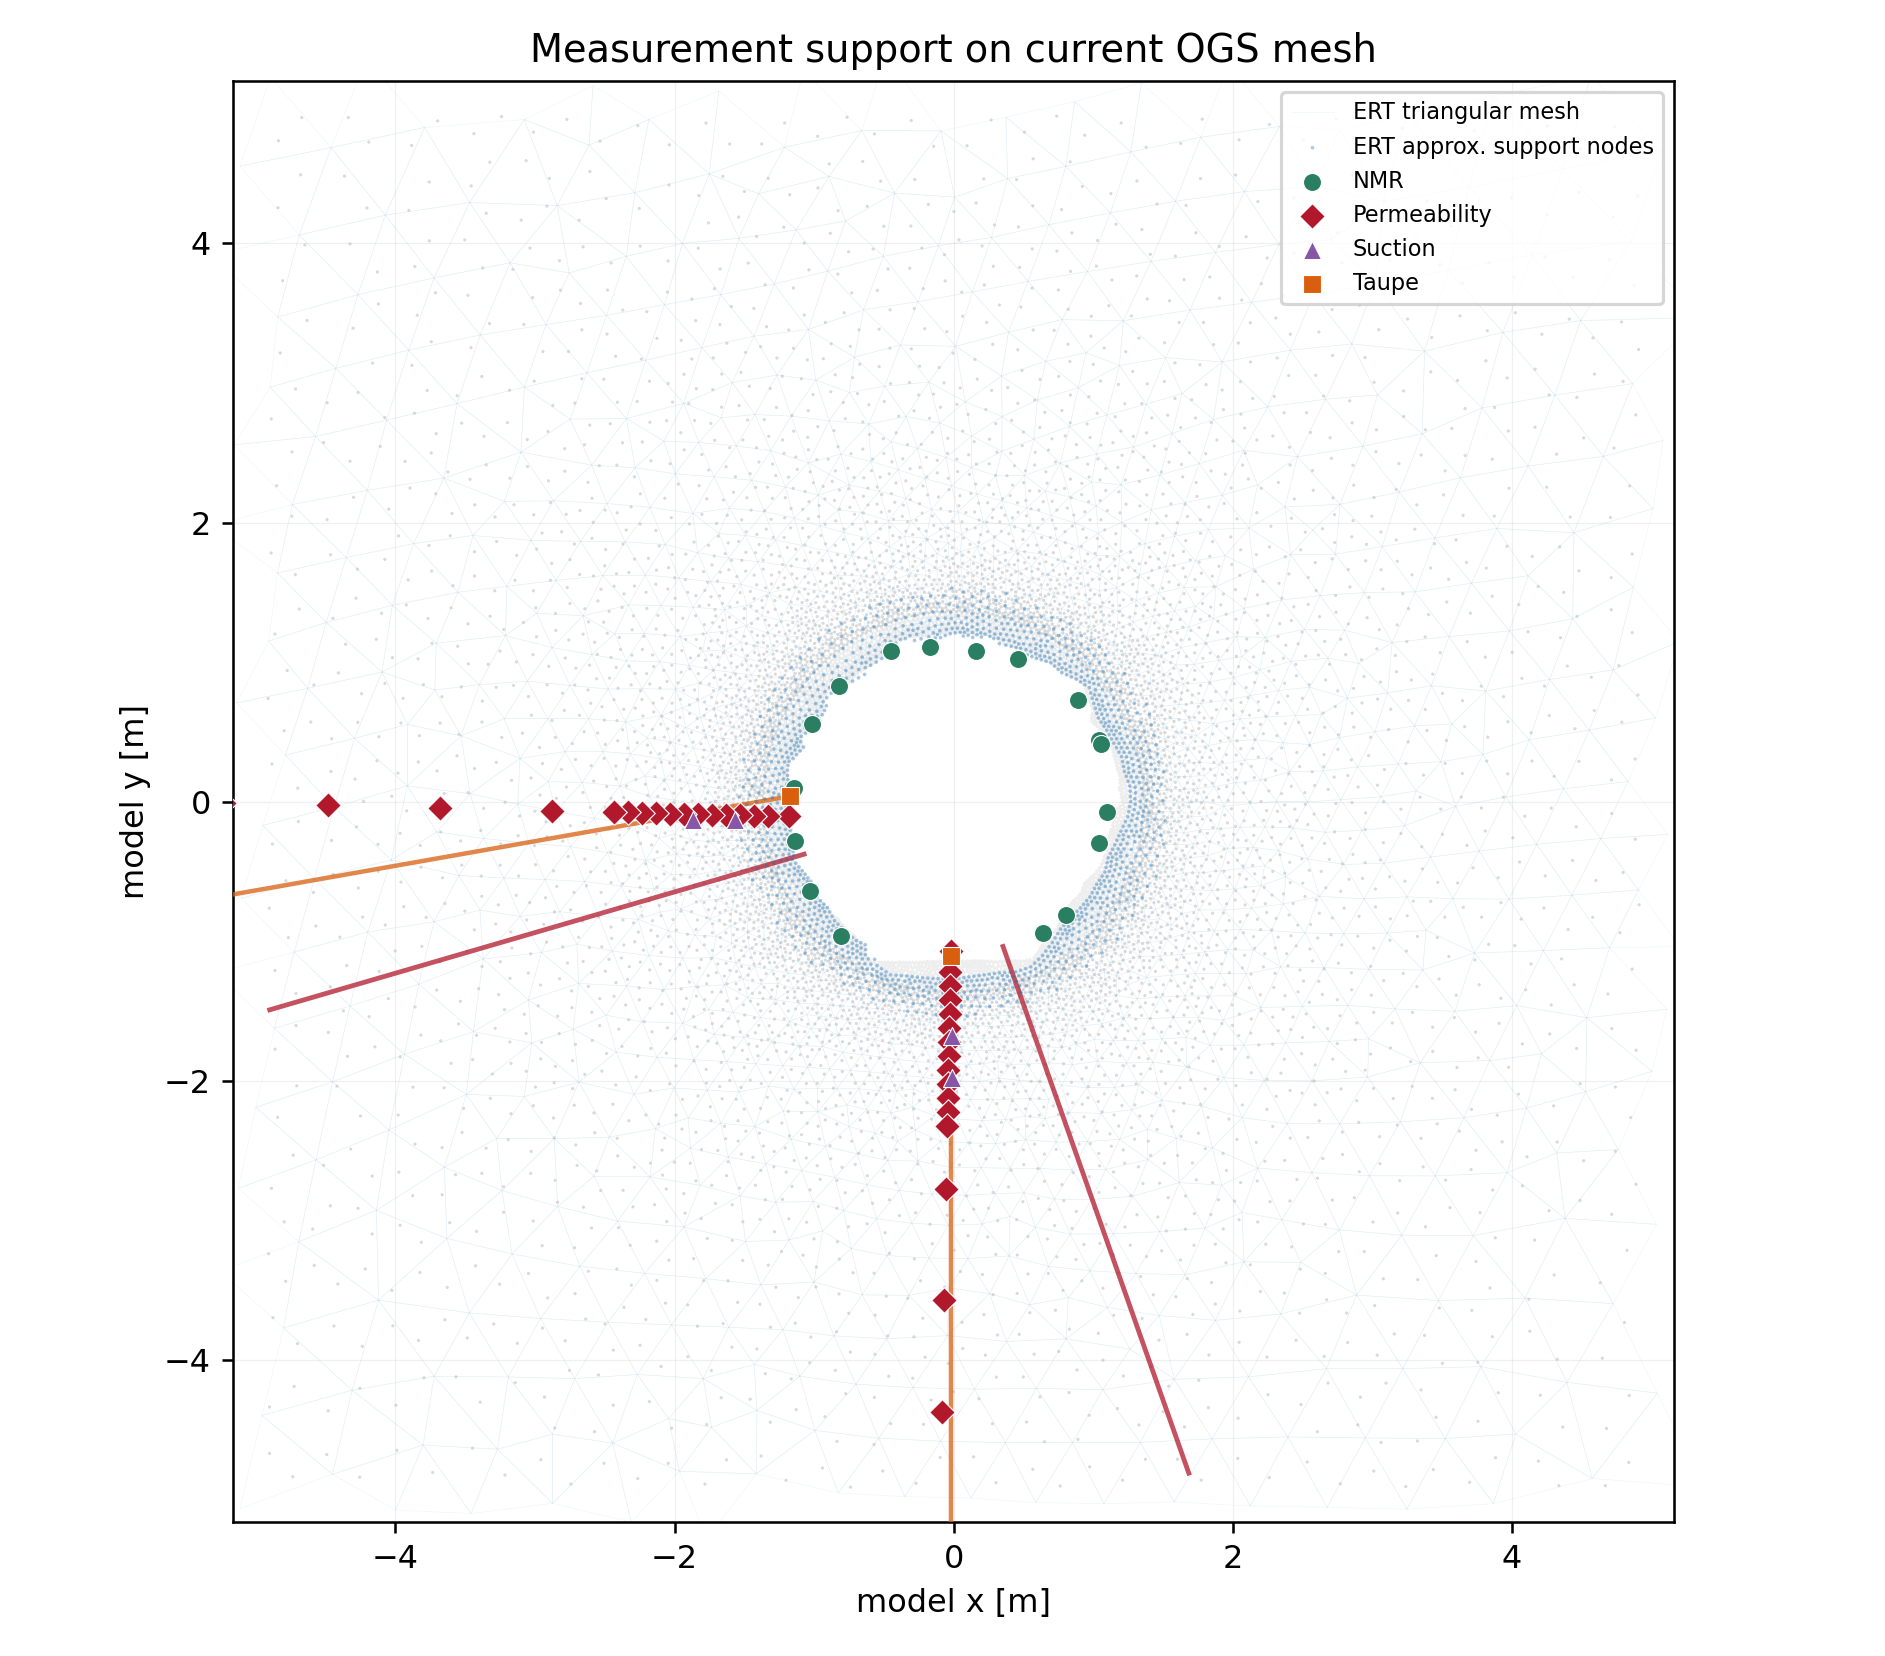
\includegraphics[width=0.90\textwidth]{figures/setup_all_measurement_locations_mesh.png}
\caption{All currently mesh-mapped measurement supports on the OGS domain.  ERT is
shown as its projected triangular mesh, with the approximate 1.5 m support subset
highlighted by mesh nodes.  NMR, Taupe/TDR, suction/RH, and permeability rows use the
processed 2D model-coordinate lookup tables.  Streams without mesh-ready coordinates
are treated separately in the Other-HM section rather than being forced onto this
mesh.}
\label{fig:setup-all-locations}
\end{figure}

\subsection{Bedding-Angle Structural Prior}

The current permeability tensor uses a fixed bedding-informed angle of \(144^\circ\)
and anisotropy ratio 2.5 everywhere.  This enters the PDE through the intrinsic
permeability tensor \(\K\) in Darcy's law: it rotates the principal directions used
to compute \(\vW=-(\krel\K/\muW)\grad\pp\).  Spatially, the current prior is global
over all OGS cells, although a later EDZ/facies model could make it local.  In time,
it is constant; it is not a measurement time series.  For inversion it should remain
a prior or fixed tensor-shape assumption unless directional permeability evidence,
ERT/Taupe support, or structural mapping justifies releasing it as a stochastic
angle field.

\begin{figure}[H]
\centering
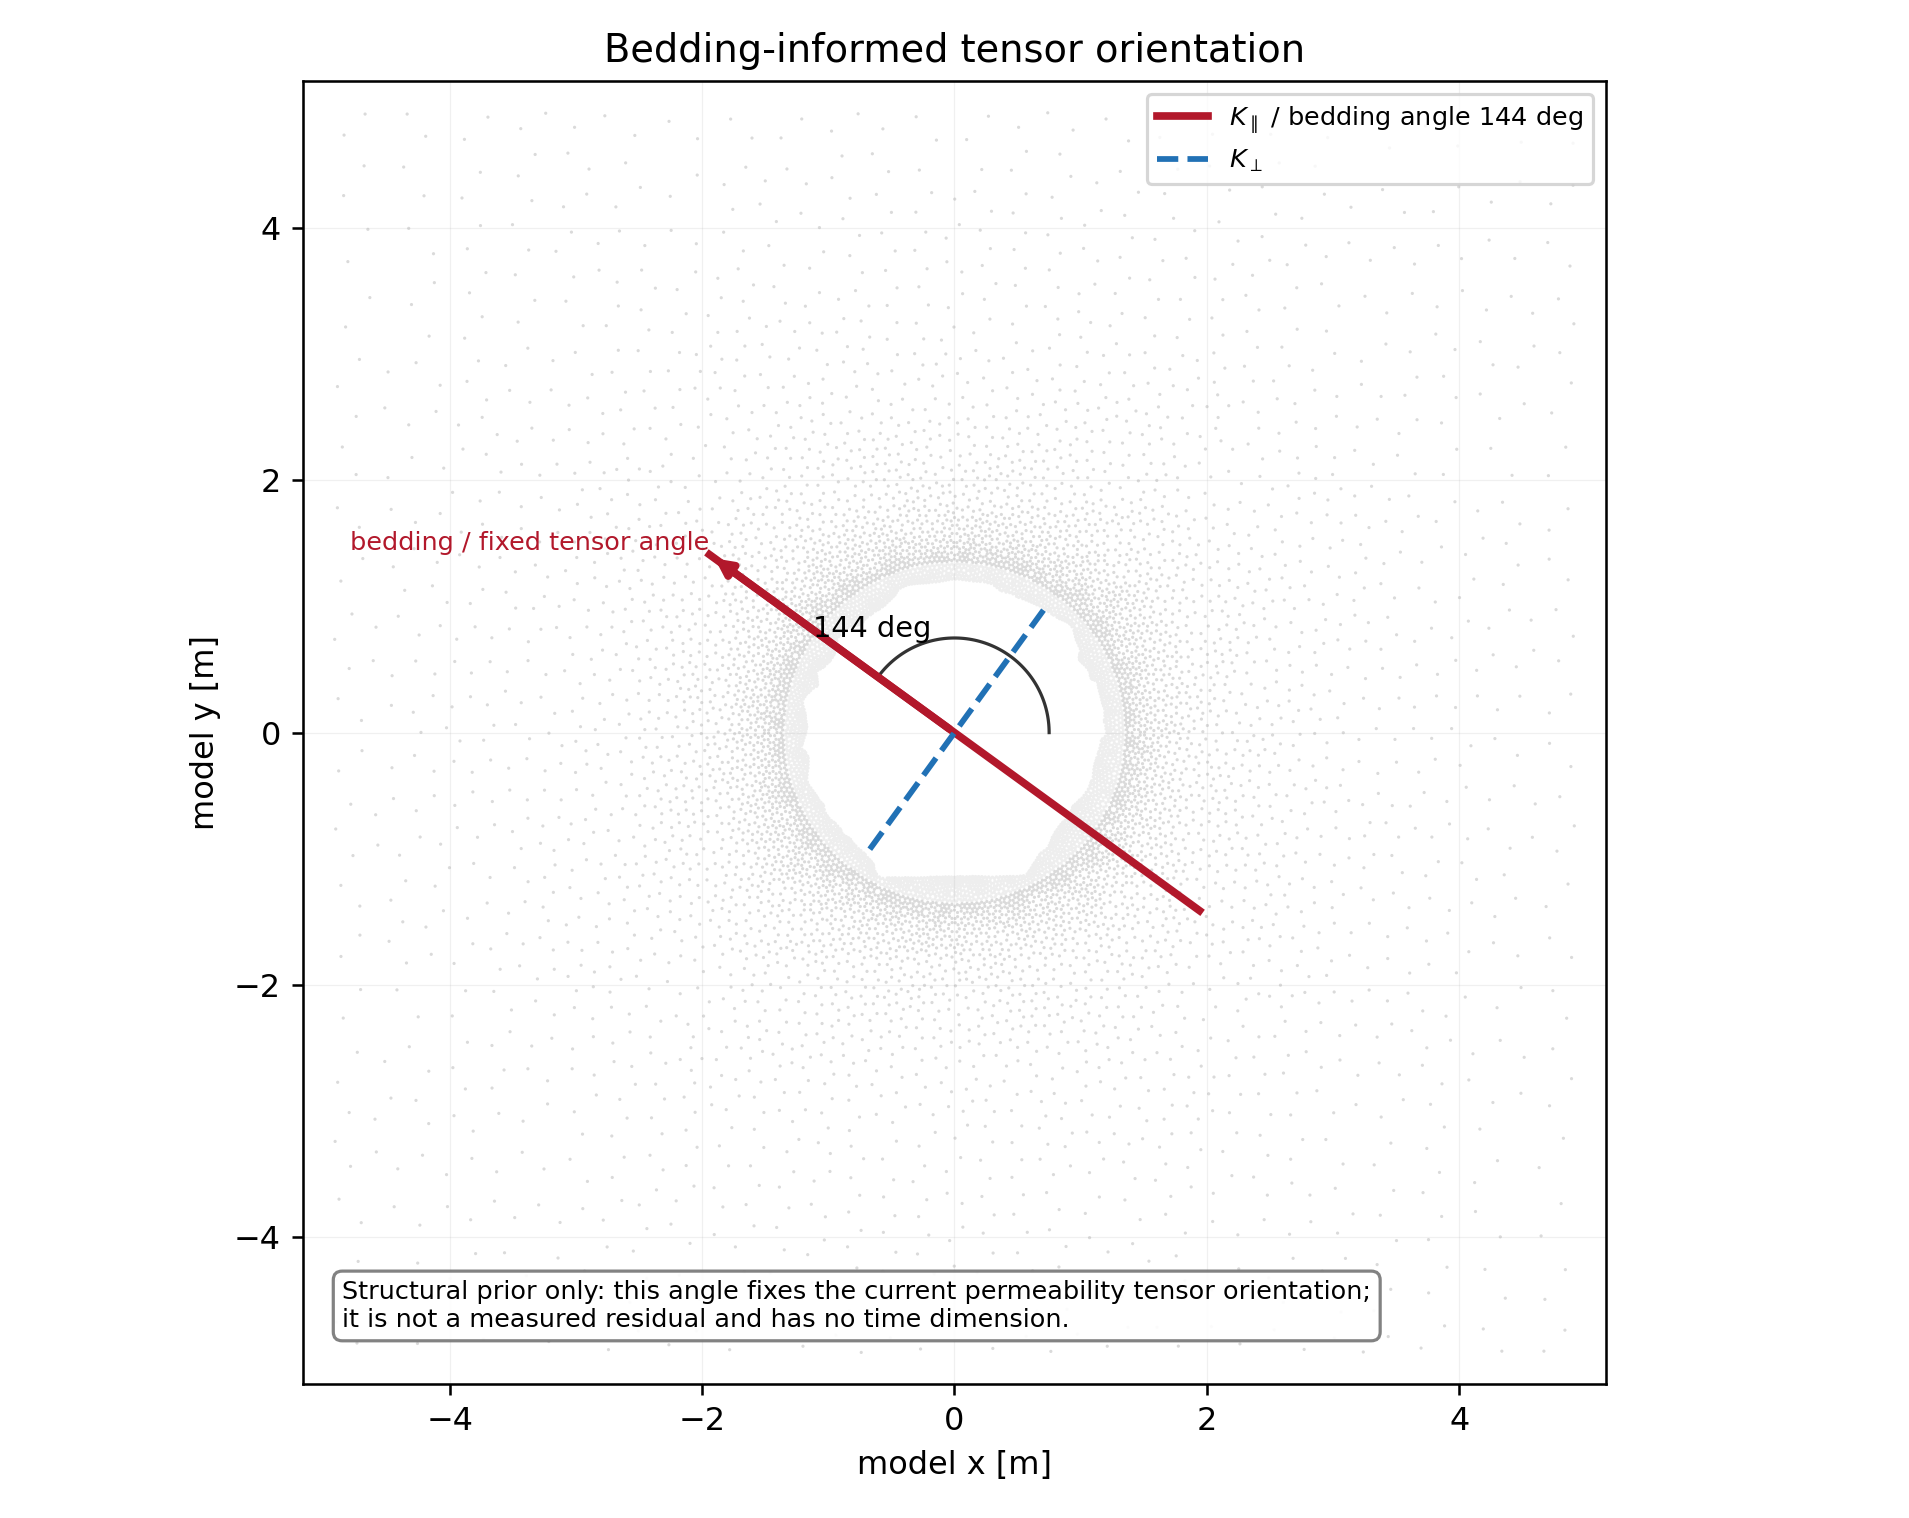
\includegraphics[width=0.86\textwidth]{figures/bedding_angle_on_mesh.png}
\caption{Bedding-angle visualisation on the current OGS mesh.  The red line is the
fixed \(K_\parallel\) direction at \(144^\circ\); the dashed blue line is the
perpendicular tensor direction.  This is a structural prior for \(\K\), not a residual
term, and therefore has no observation time or measurement likelihood of its own.}
\label{fig:bedding-angle}
\end{figure}

\subsection{Direct Permeability Residual}

The pulse-test likelihood compares the predicted directional interval permeability to
the interpreted permeability:
\[
r_i^{k}=\log_{10} k_{i,\mathrm{pred}}-\log_{10} k_{i,\mathrm{obs}},
\qquad
\Phi_k=\frac{1}{2}\sum_i w_i\left(\frac{r_i^k}{0.5}\right)^2 .
\]
The operator uses a weighted arithmetic average of \(\bm e_i^\top\K\bm e_i\) over
selected cells.  Duplicate rows with the same campaign, segment, depth, and observed
log10 value share unit weight.  This avoids over-counting repeated workbook rows but
does not fully solve the same-support conflict: 30 active support cells exist, 24
are repeated, and 16 span at least two log10 units.  The worst recorded conflict is
cell 4648 at BCD-A32, 0.85--0.87 m, with observed range 6.94885 log10 units.

\begin{figure}[H]
\centering
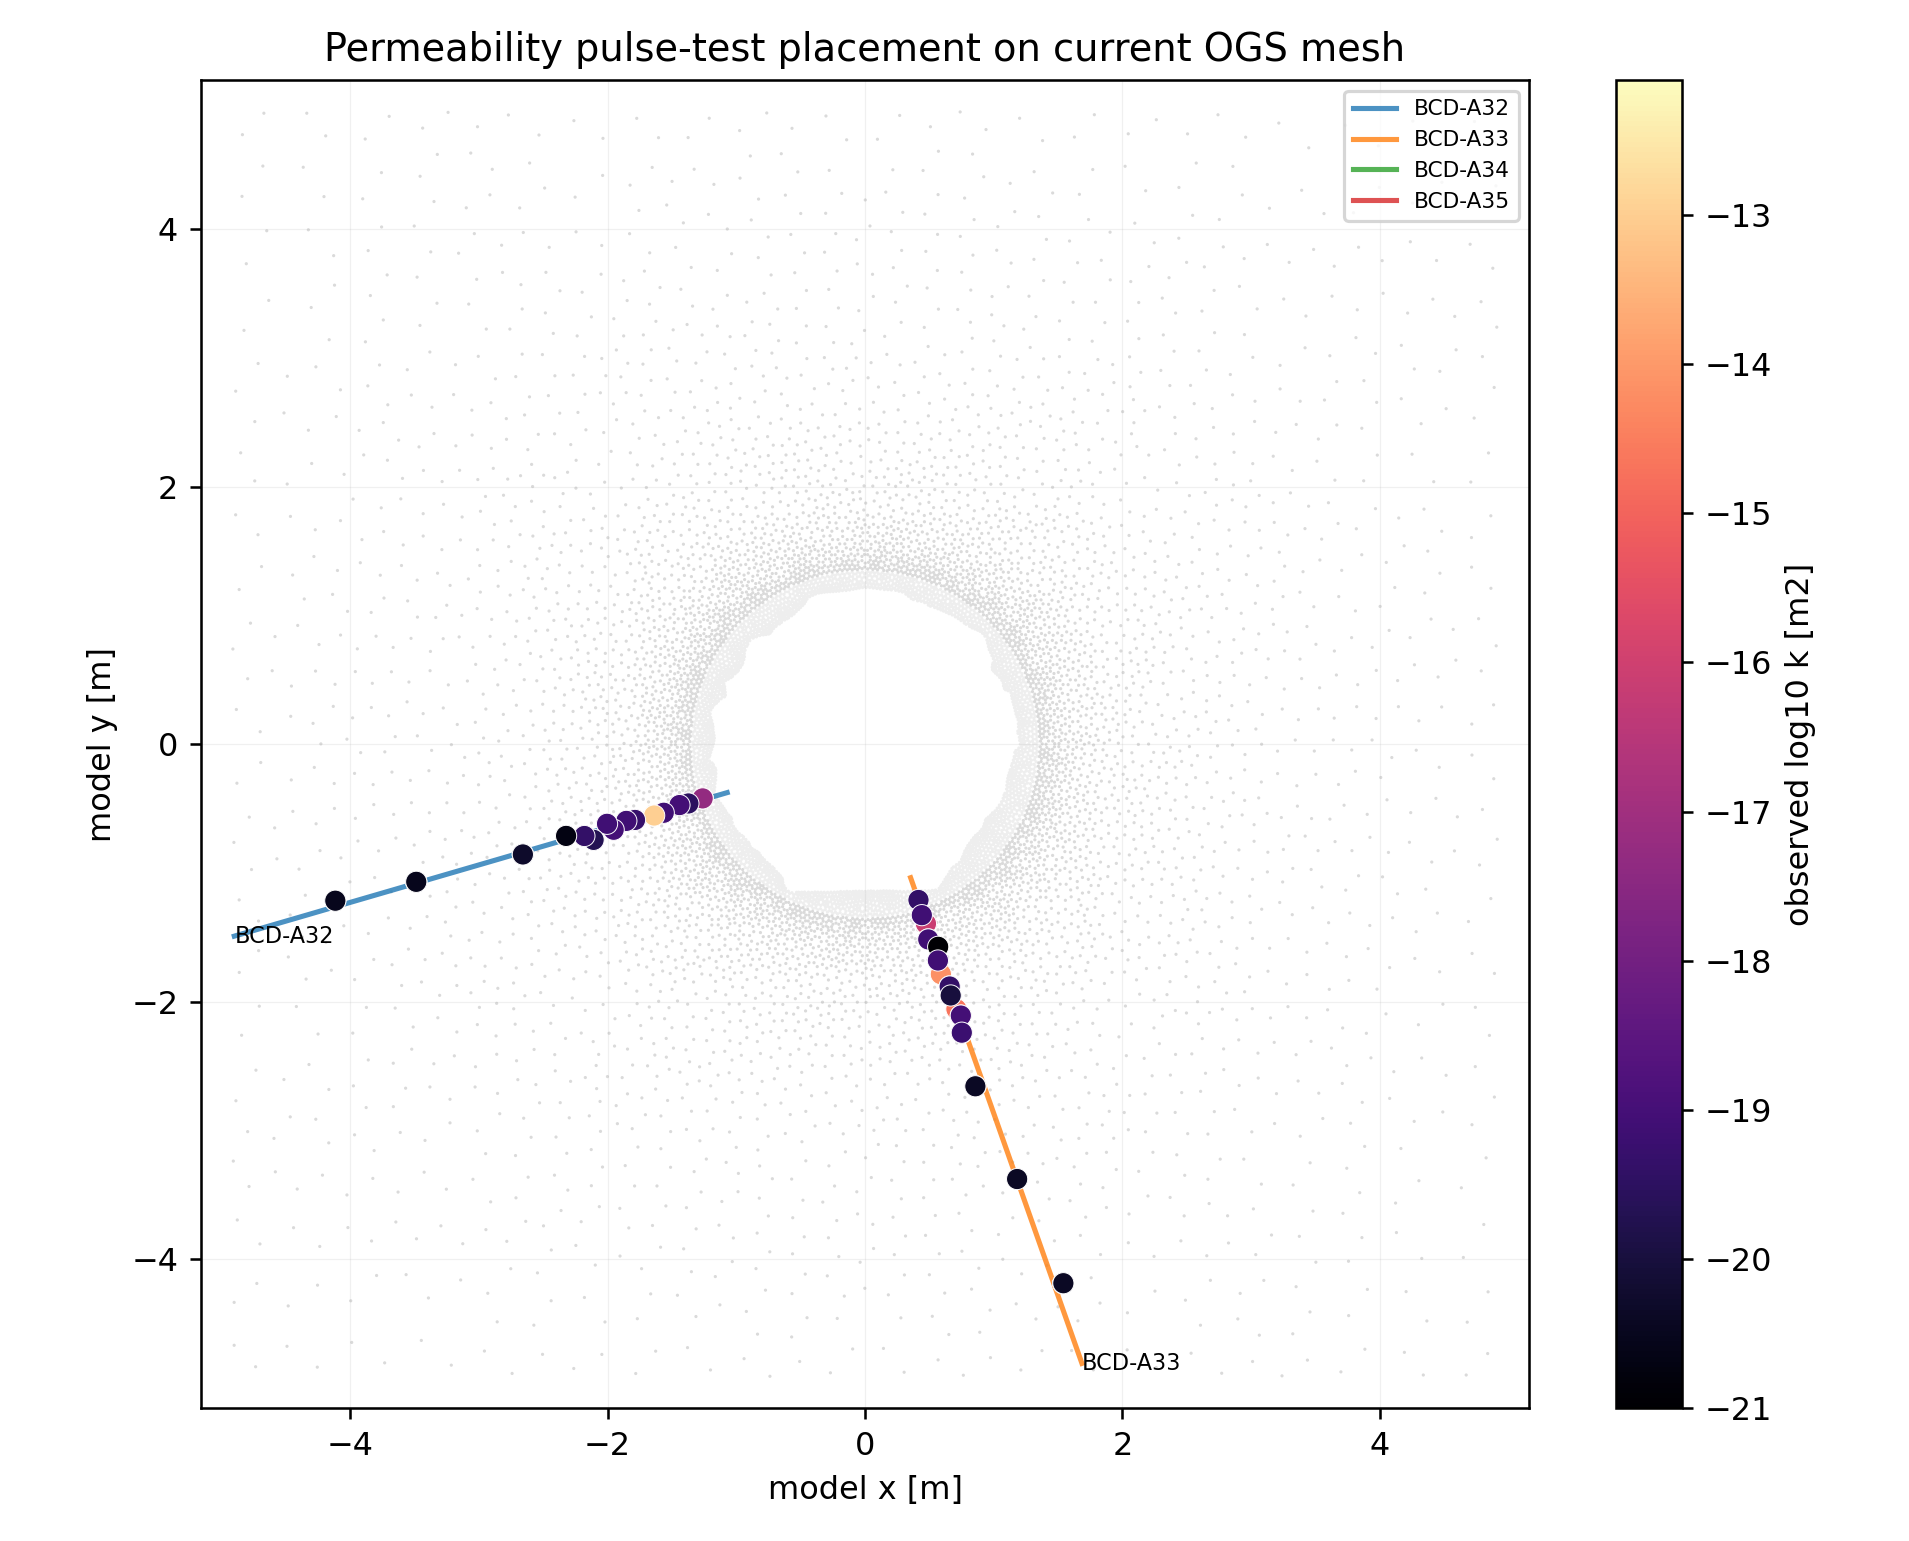
\includegraphics[width=0.86\textwidth]{figures/permeability_mesh_placement.png}
\caption{Direct permeability placement.  The active mapped pulse-test supports lie on
the BCD-A32 and BCD-A33 characterization boreholes around the current niche mesh.
Points are active support cells coloured by interpreted \(\log_{10}k\); the plotted
borehole lines show where the interval operator samples the current OGS cell field.}
\label{fig:permeability-placement}
\end{figure}

\paragraph{Open/closed twin filter.}
The source catalogue contains open-twin, closed-twin, and unlabeled permeability
rows.  The active direct-permeability objective uses only the open-twin rows that
also have accepted current-mesh support: BCD-A32 and BCD-A33.  No closed-twin row
enters the present OGS fit.

\begin{longtable}{@{}L{0.16\textwidth}L{0.24\textwidth}L{0.14\textwidth}Y@{}}
\caption{Direct-permeability twin and support usage.}\\
\toprule
Source class & Catalogue rows & Current use & Reason \\
\midrule
\endfirsthead
\toprule
Source class & Catalogue rows & Current use & Reason \\
\midrule
\endhead
\bottomrule
\endlastfoot
Open twin, mapped current niche & BCD-A32: 38 positive rows; BCD-A33: 37 positive rows plus 4 nonpositive/missing values. & Active: 75 positive rows. & These are the only open-twin permeability rows with accepted BCD-A32/A33 segment geometry and inside-mesh OGS support. \\
Open twin, historical context & BFM-D19: 8 positive 2021 rows. & Inactive context. & The rows are open-twin evidence, but no accepted segment geometry/support exists for the current 2D OGS objective. \\
Closed twin & BCD-A27: 15 positive 2021 rows; BCD-A34: 15 positive 2024 rows; BCD-A35: 12 positive 2024 rows. & Inactive. & These belong to the closed twin or map outside the current open-niche mesh support, so they should not be fitted in the present open-niche objective. \\
Unlabeled historical rows & BCD-A24/25/26: 75 rows. & Inactive. & These rows do not have a usable open-twin assignment and accepted endpoint geometry for the current support operator. \\
\end{longtable}

\begin{figure}[H]
\centering
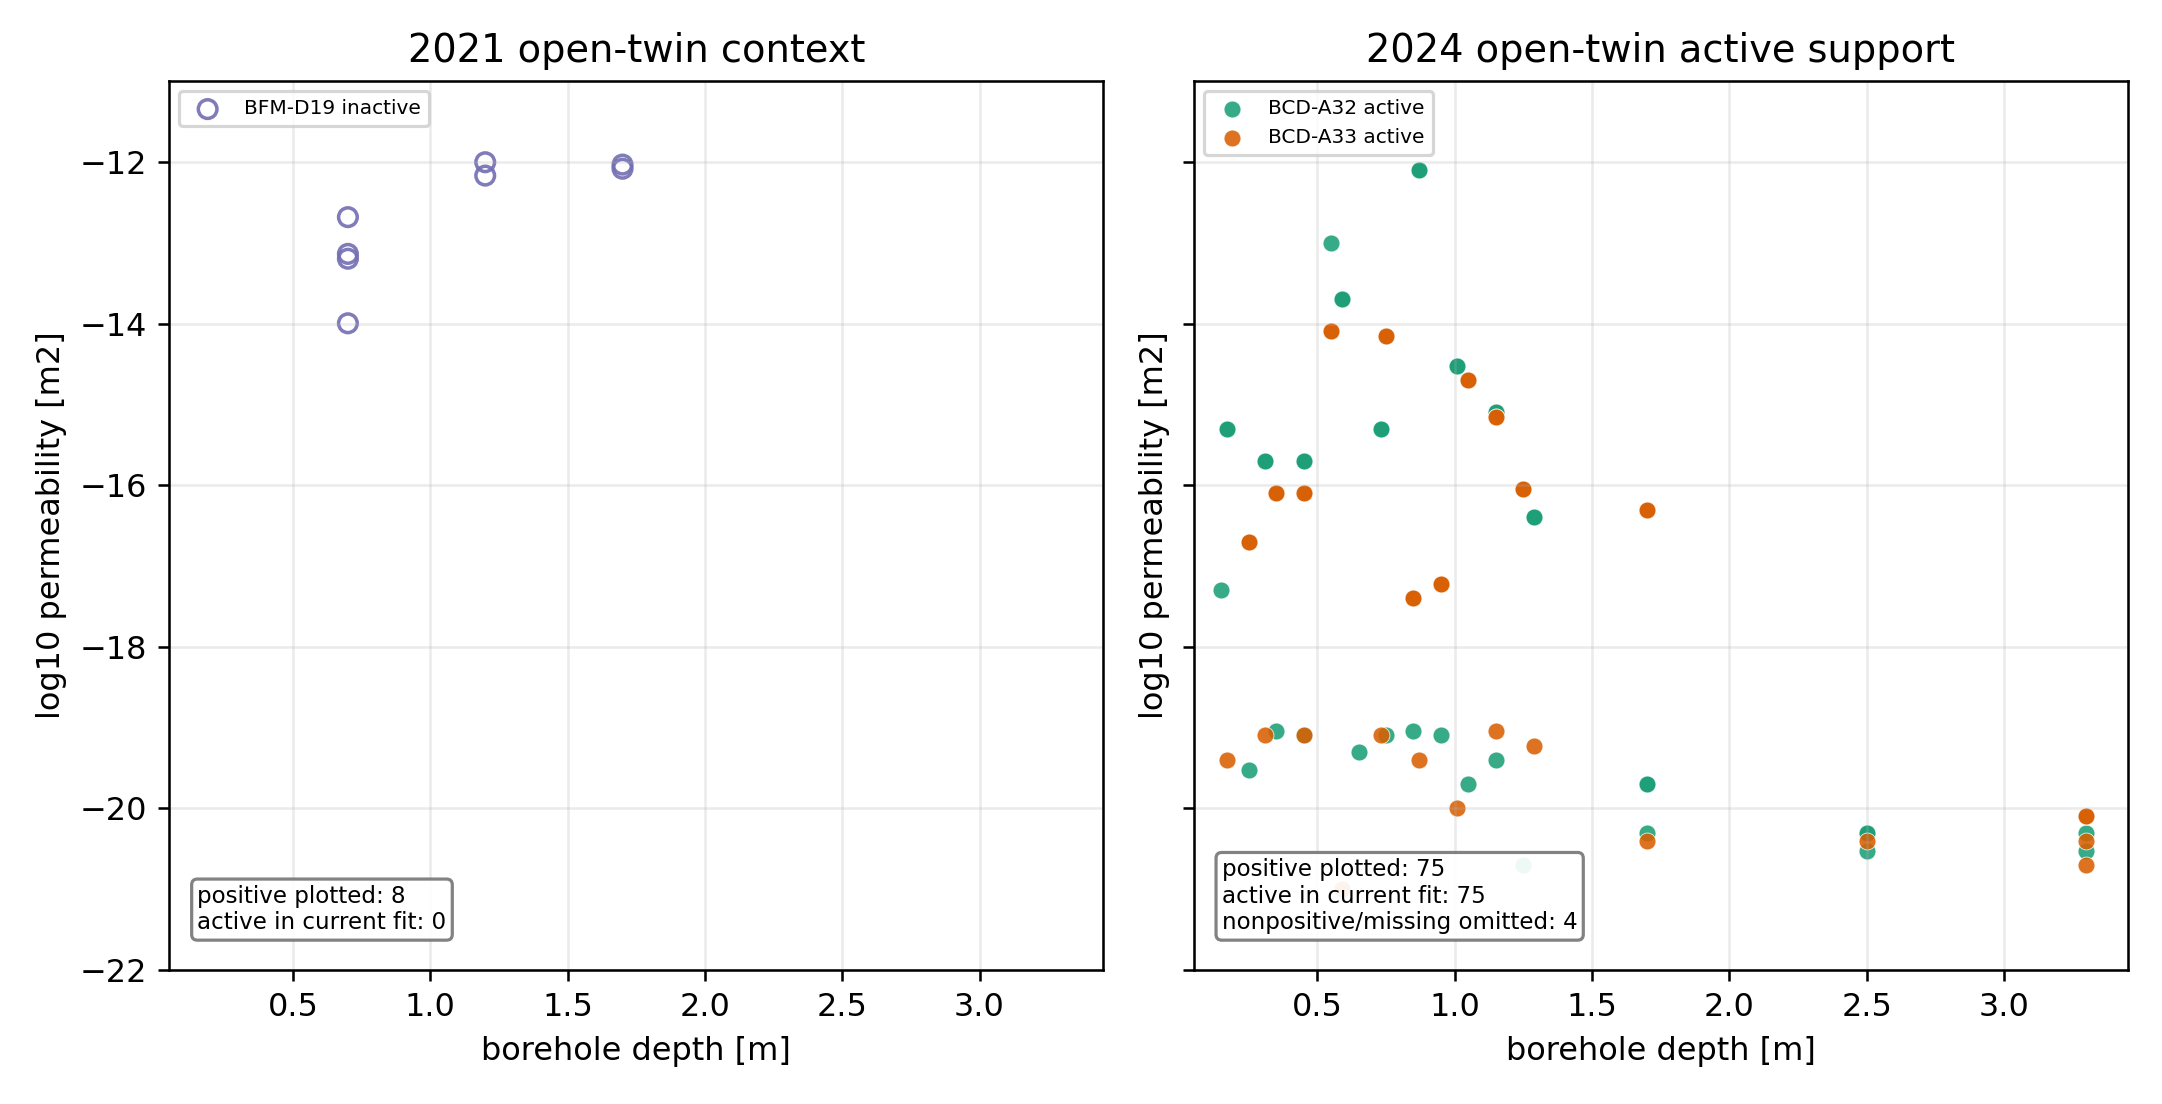
\includegraphics[width=0.98\textwidth]{figures/permeability_open_twin_by_campaign.png}
\caption{Open-twin permeability rows split by campaign year with identical
depth and \(\log_{10}k\) axes.  The 2021 BFM-D19 rows are open-twin context but
inactive because their segment geometry is not accepted for the current OGS support
operator.  The 2024 BCD-A32/A33 rows are the active open-twin support; four
nonpositive or missing BCD-A33 values are omitted from the logarithmic plot.}
\label{fig:permeability-open-campaign}
\end{figure}

\begin{figure}[H]
\centering
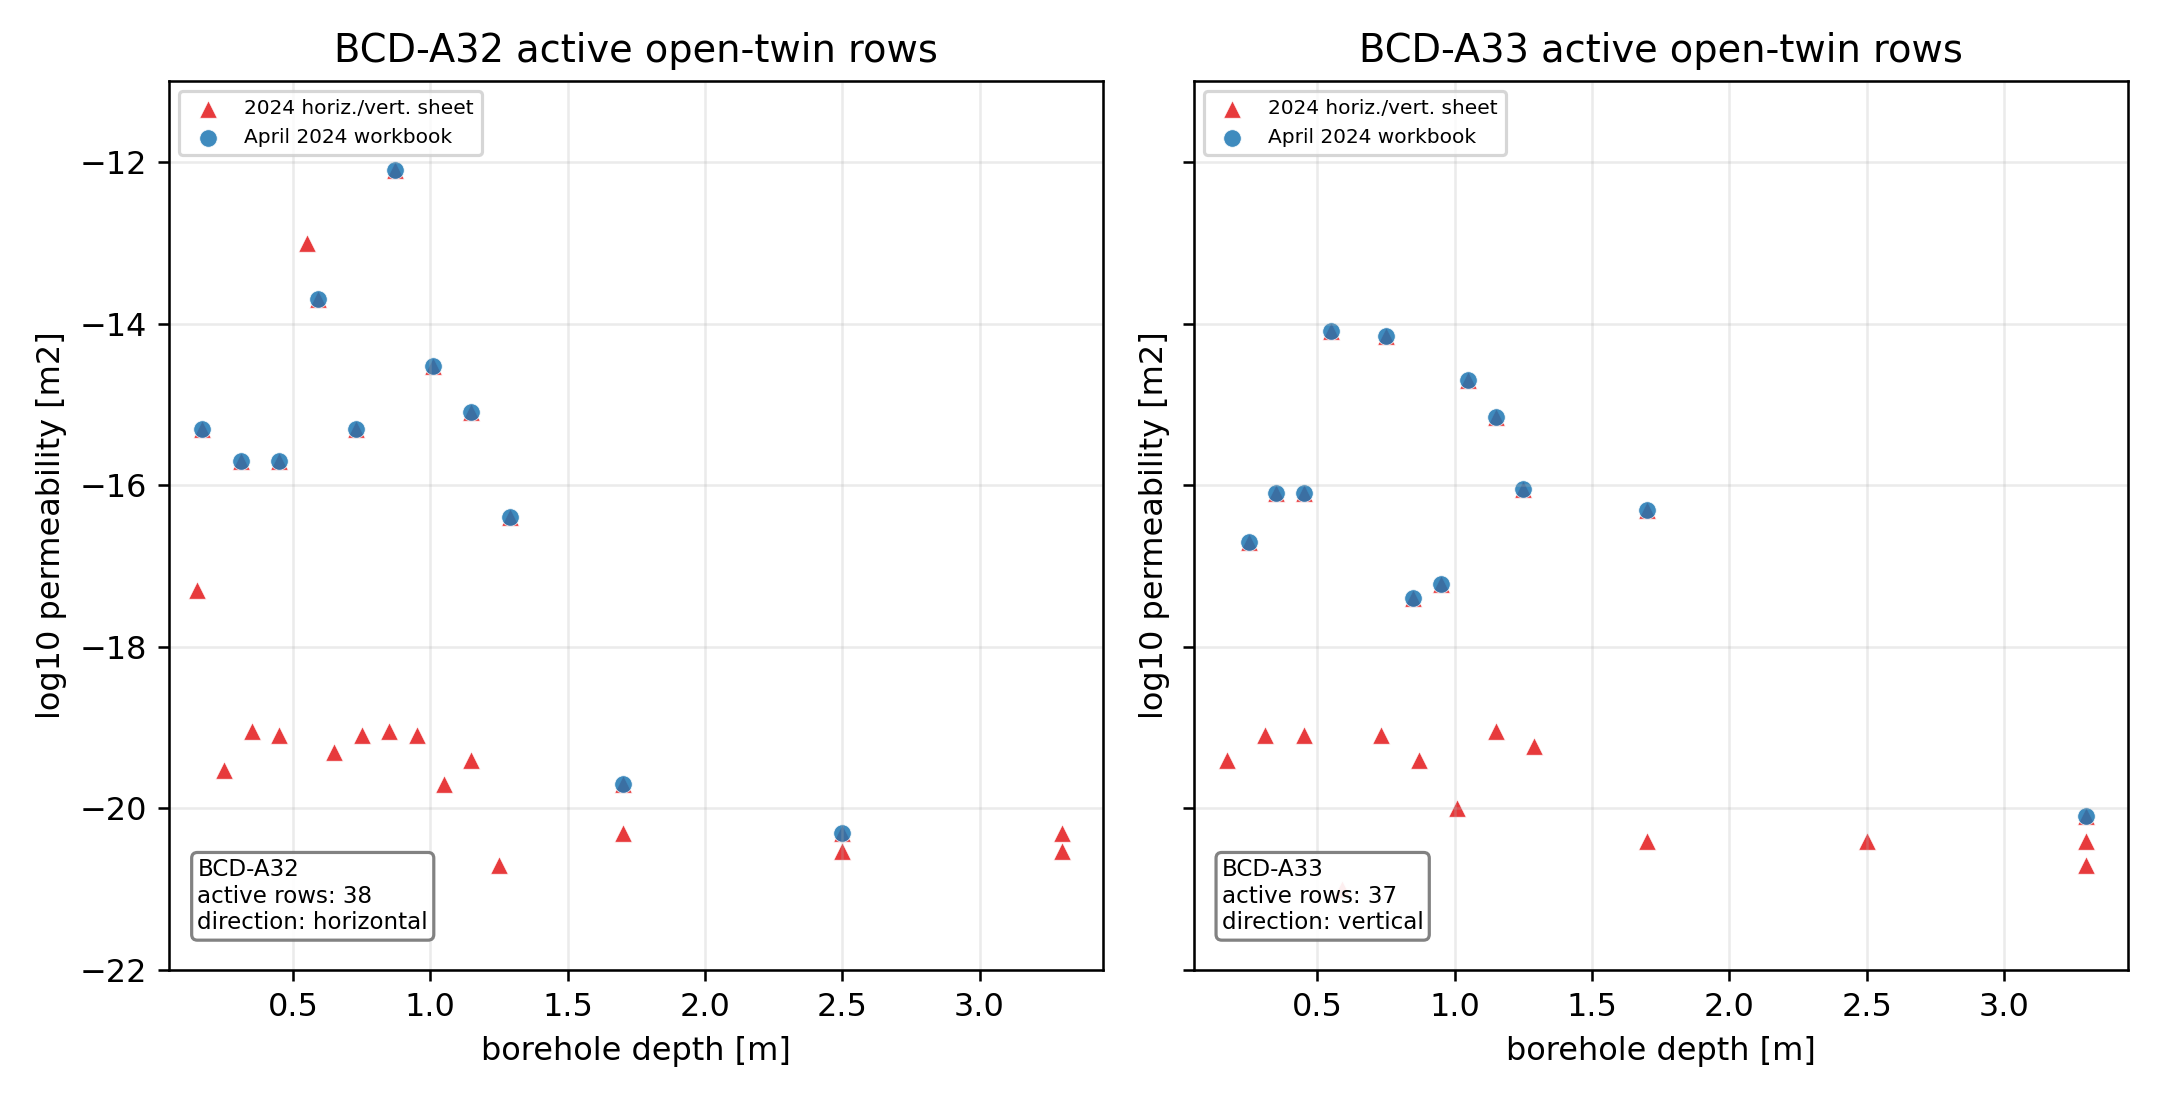
\includegraphics[width=0.98\textwidth]{figures/permeability_active_open_by_borehole.png}
\caption{Active open-twin permeability rows split by borehole with identical
depth and \(\log_{10}k\) axes.  BCD-A32 contributes the horizontal active rows and
BCD-A33 contributes the vertical active rows.  The two marker styles separate the
April 2024 workbook rows from the additional 2024 horizontal/vertical source sheet.}
\label{fig:permeability-active-borehole}
\end{figure}

\paragraph{Inversion incorporation.}
The permeability rows enter directly in the hydraulic PDE through \(\K(\bm x)\) in
Darcy's law and therefore affect pressure diffusion, saturation evolution, and all
water-content proxies.  Spatially, each row is treated as an interval or small
cell-set average along the mapped borehole segment, not as an exact point
measurement.  Temporally, the active interpreted pulse-test \(k\) values are used
as quasi-static material observations from the 2024 open-twin BCD-A32/A33 rows
rather than as transient pressure-decay curves in the OGS time loop.  The 2021
open-twin BFM-D19 rows and all closed or unlabeled rows remain context only until
their geometry, twin assignment, and support policy are accepted.  The active
residual is the duplicate-weighted Gaussian residual in \(\log_{10}k\) with
\(\sigma=0.5\); changing this support or likelihood policy is one of the main
remaining decisions before calling the permeability field final.

\subsection{NMR Residual}

The active residual is
\[
r_i^{\mathrm{NMR,raw}} =
\frac{\thetaw_{\mathrm{model}}(\bm x_i,t_i)-\thetaw_{i,\mathrm{NMR}}}
     {\sigma_i},
\qquad
\thetaw_{\mathrm{model}}=\npor\Sat .
\]
The key caveat is semantic: NMR observes total hydrogen-bearing water, not only the
mobile liquid saturation represented by Richards' equation.  A bound-water audit found
that 315 of 464 NMR target rows exceed the maximum possible model-side
\(\thetaw=\npor\Sat\) if interpreted directly as mobile water, and 162 of 287 usable
Niche-4 mapped rows exceed \(n=0.105\).  A safer provisional final residual is the
within-label anomaly:
\[
r_i^{\mathrm{NMR,anom}} =
\left(\thetaw_{\mathrm{model},i}-\overline{\thetaw_{\mathrm{model}}}_{\ell(i)}\right)
-
\left(\thetaw_{\mathrm{obs},i}-\overline{\thetaw_{\mathrm{obs}}}_{\ell(i)}\right),
\]
where \(\ell(i)\) is the observation-family/label group.  This cancels constant
bound/interlayer/campaign offsets to first order.

\begin{figure}[H]
\centering
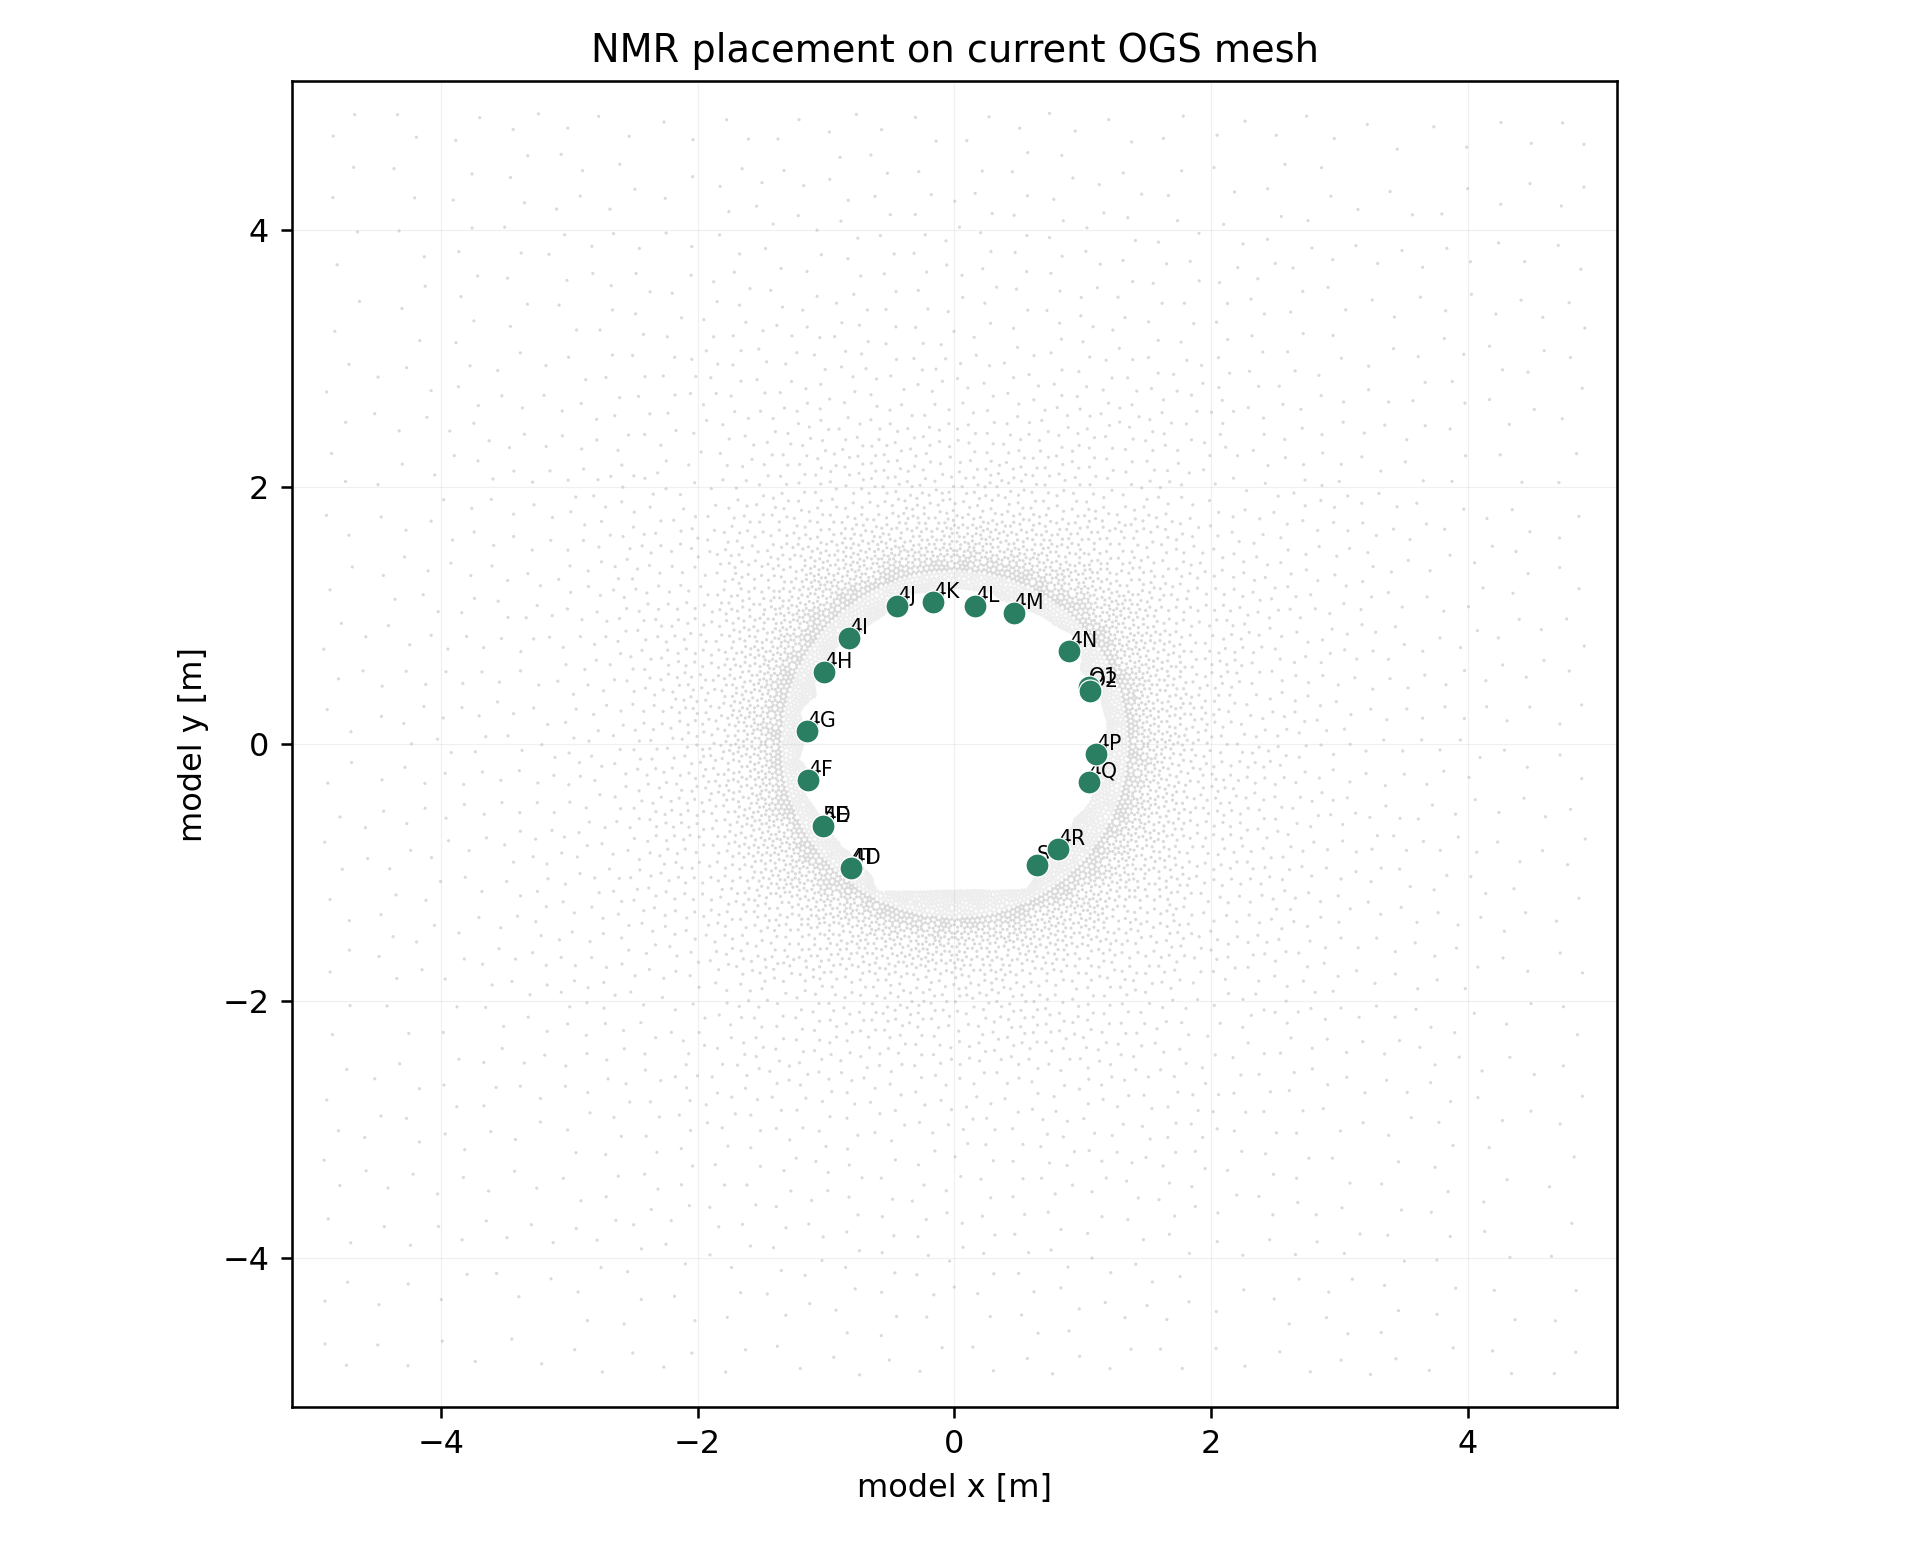
\includegraphics[width=0.86\textwidth]{figures/nmr_mesh_placement.png}
\caption{NMR placement.  The NMR labels are plotted in the same 2D model coordinates
used by the current observation operator.  These coordinates define where
\(\thetaw=\npor\Sat\) is sampled from OGS output for the active raw-NMR objective and
for the proposed within-label anomaly residual.}
\label{fig:nmr-placement}
\end{figure}

\begin{figure}[H]
\centering
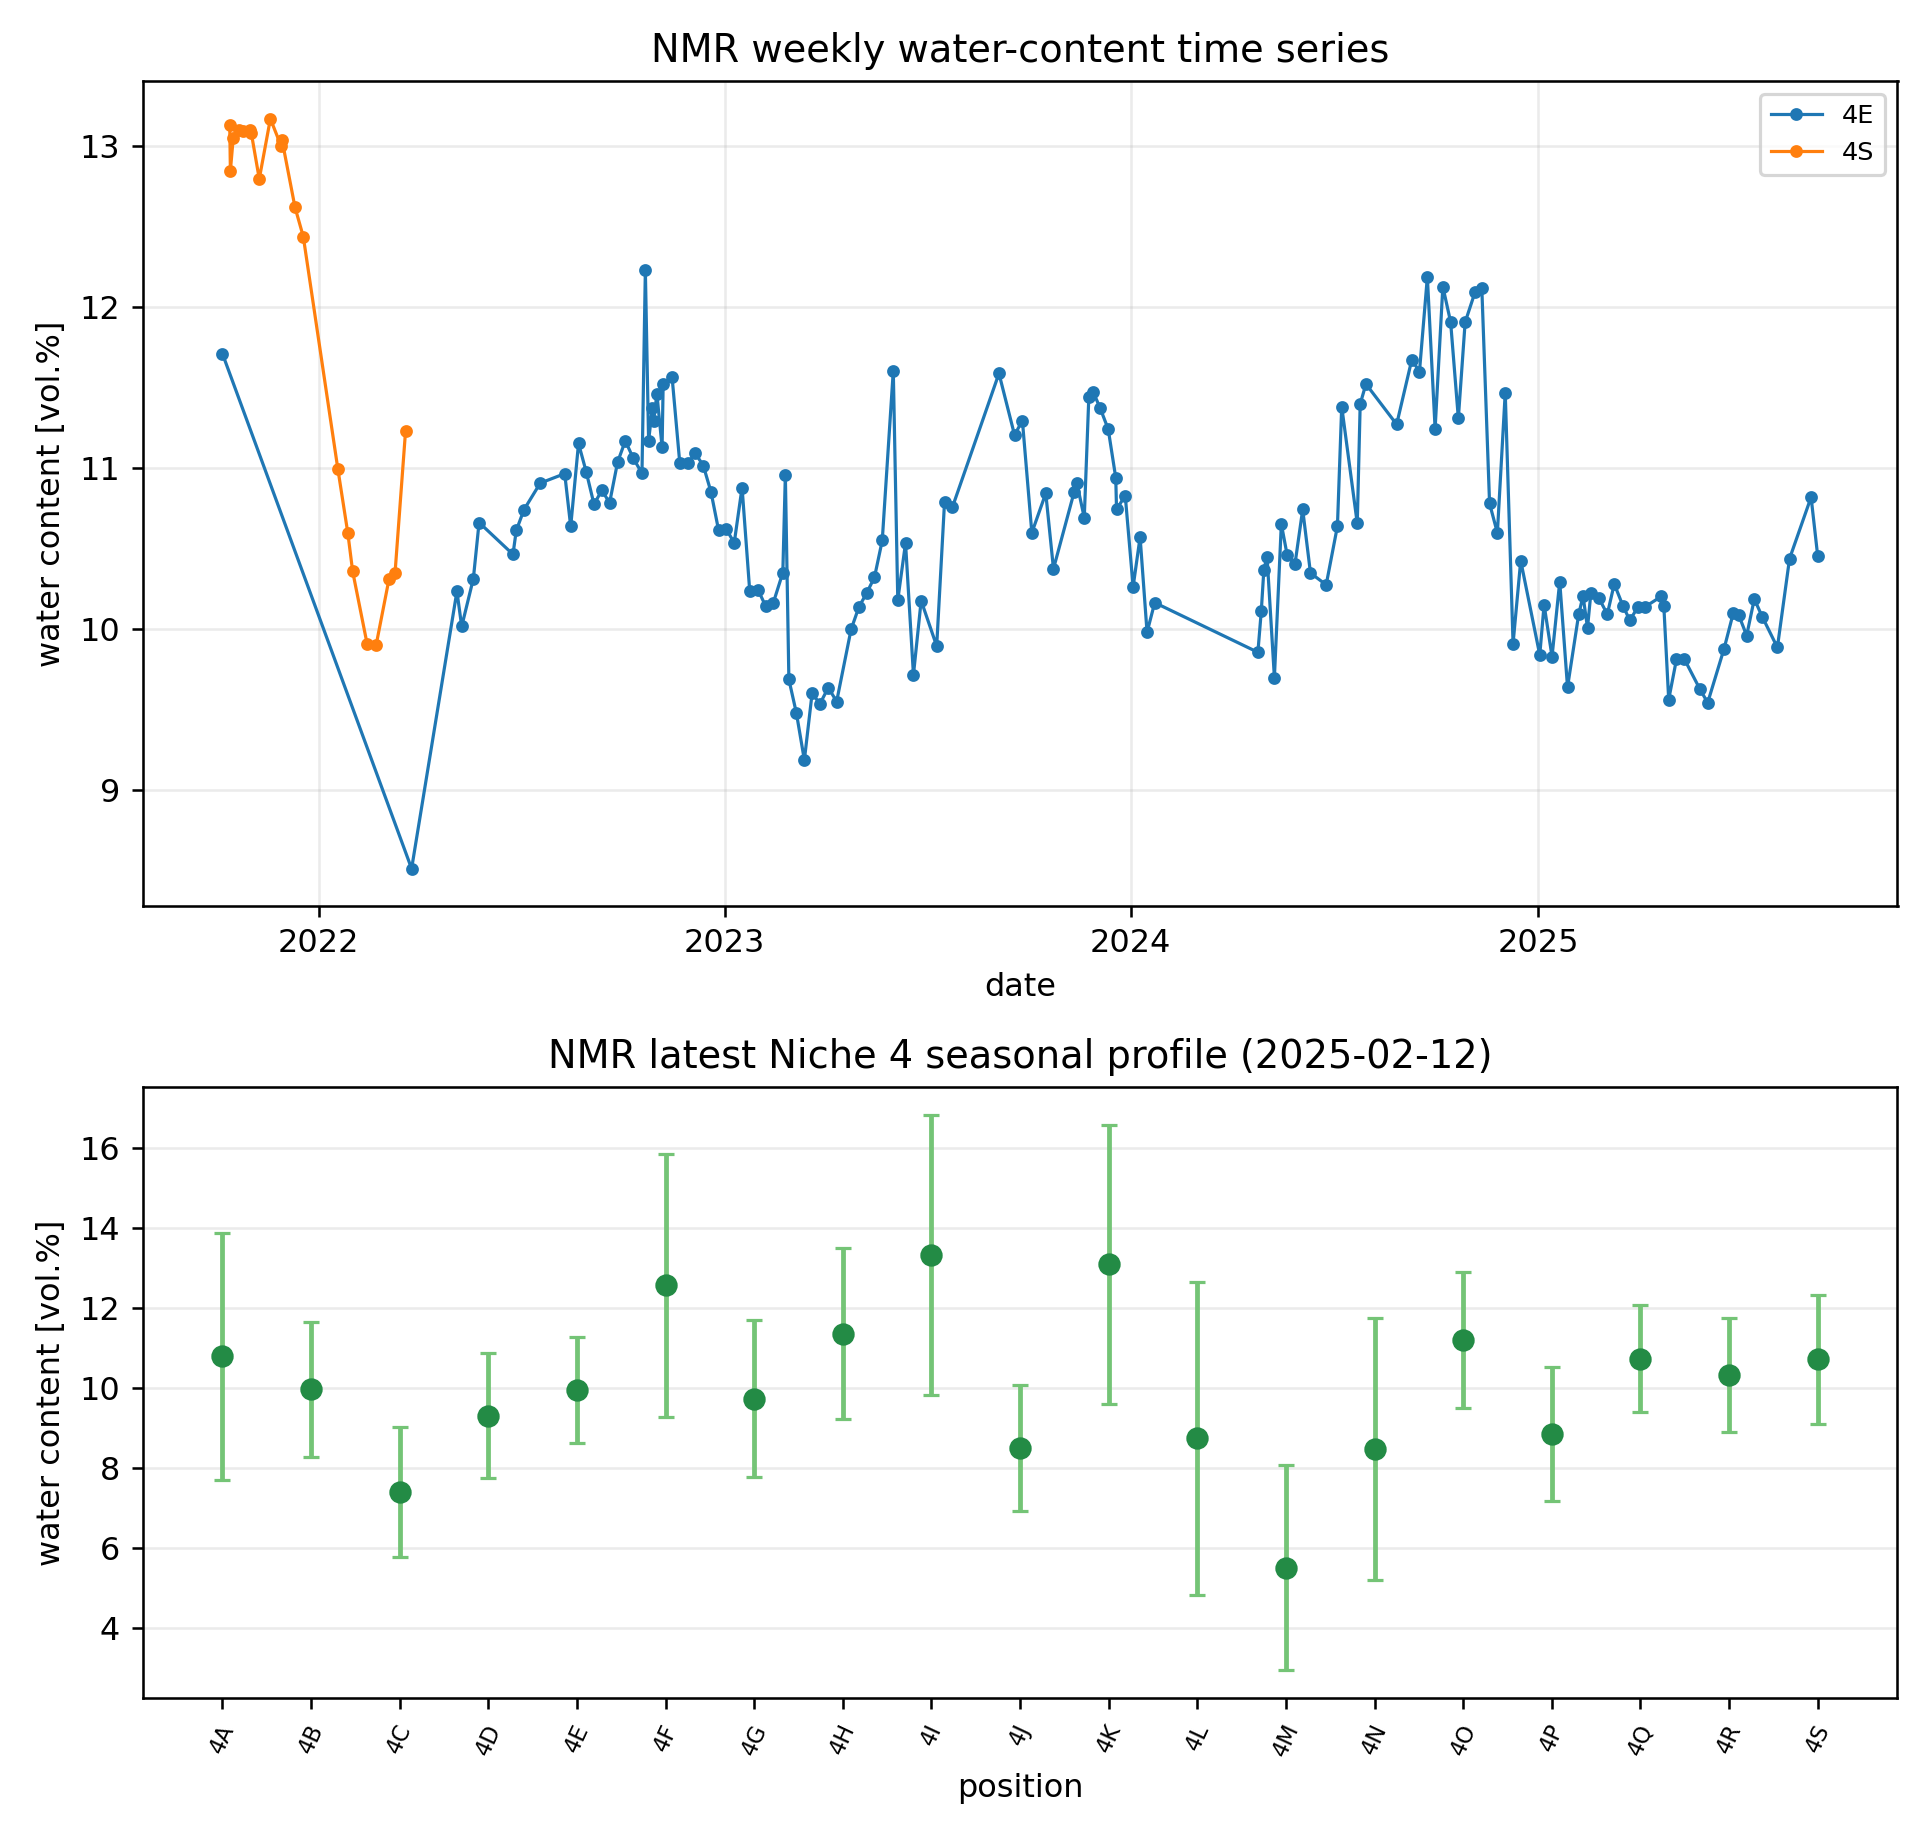
\includegraphics[width=0.98\textwidth]{figures/nmr_data_visualisation.png}
\caption{NMR measured-data visualisation.  The upper panel shows weekly water-content
time series for stations 4E and 4S.  The lower panel shows the latest Niche 4 seasonal
profile with reported 95\% confidence intervals.  The values are total NMR
water-content observations in vol.\%, so they should not be read as mobile
\(nS_\ell\) without a bound/interlayer-water policy.}
\label{fig:nmr-data}
\end{figure}

\paragraph{Inversion incorporation.}
NMR enters the liquid-mass part of the TRM model through the sampled state
\(\thetaw(\bm x,t)=\npor\Sat(\bm x,t)\), where \(\Sat\) is produced by the
Richards retention law from liquid pressure.  Spatially, each label samples the
nearest accepted OGS support point in the current 2D lookup; Niche 3 rows are useful
context but are outside the present Niche 4 fit.  In time, NMR rows are matched to
OGS output times near the observation dates, giving 192 active rows in the current
objective.  The present residual is raw absolute \(\theta\), but the more defensible
next residual is the within-label anomaly because it removes constant NMR bound-water
offsets that the PDE does not model.

\subsection{ERT Residual Candidate}

ERT should enter only through a forward observation operator:
\[
\Sat(\bm x,t)\rightarrow \thetaw(\bm x,t)=\npor\Sat(\bm x,t)
\rightarrow \rho_{\mathrm{pred}}(\bm x,t)
\rightarrow \Oop_{\mathrm{ERT}}[\rho_{\mathrm{pred}}],
\]
with a log-resistivity residual
\[
r^{\mathrm{ERT}} =
\log_{10}\rho_{\mathrm{pred}}-\log_{10}\rho_{\mathrm{ERT}} .
\]
The current default first-test conversion is
\(\rho_{\Omega m}=1.108\,\theta^{-1.58}\) over \(0.01\le\theta\le0.18\).  It is a
local empirical relation, not a universal claystone saturation law.  ERT can be
powerful for heterogeneity because it samples dense spatial fields through time, but
it is also the stream most vulnerable to correlated inversion pixels, coordinate
support errors, and clay surface-conduction bias.

\begin{figure}[H]
\centering
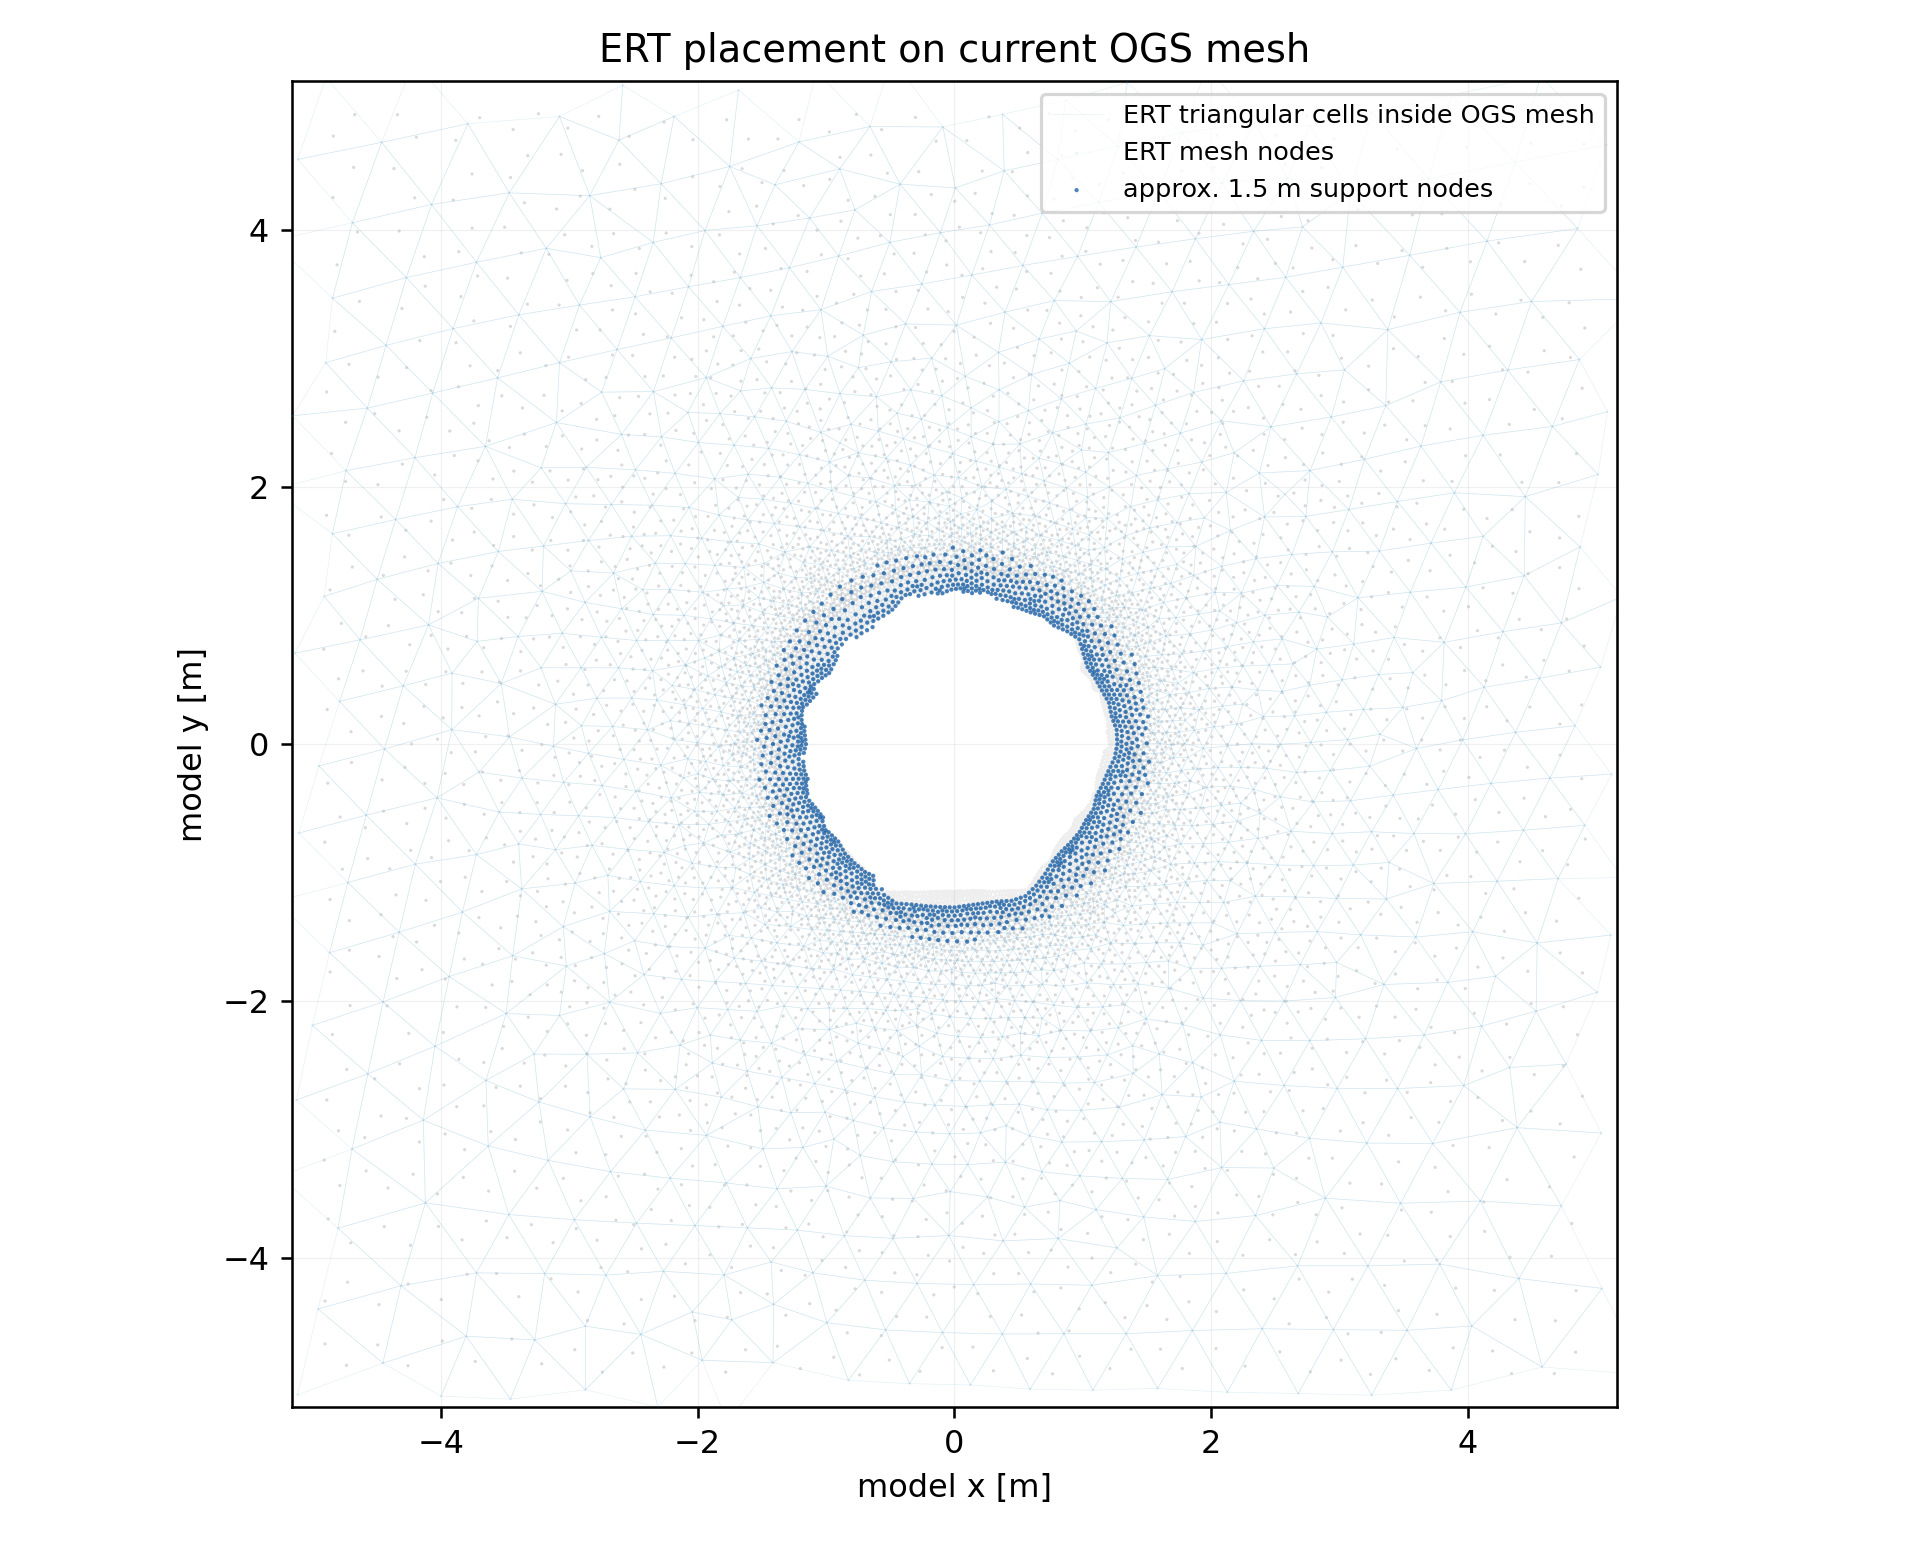
\includegraphics[width=0.86\textwidth]{figures/ert_mesh_placement.png}
\caption{ERT placement.  The pale wireframe is the projected ERT triangular mesh
inside the current OGS domain, and the darker dots are mesh nodes belonging to the
current approximate 1.5 m centre-support subset.  This is the spatial support that
would be sampled or aggregated by an ERT observation operator after the transform and
covariance gates are accepted.}
\label{fig:ert-placement}
\end{figure}

\begin{figure}[H]
\centering
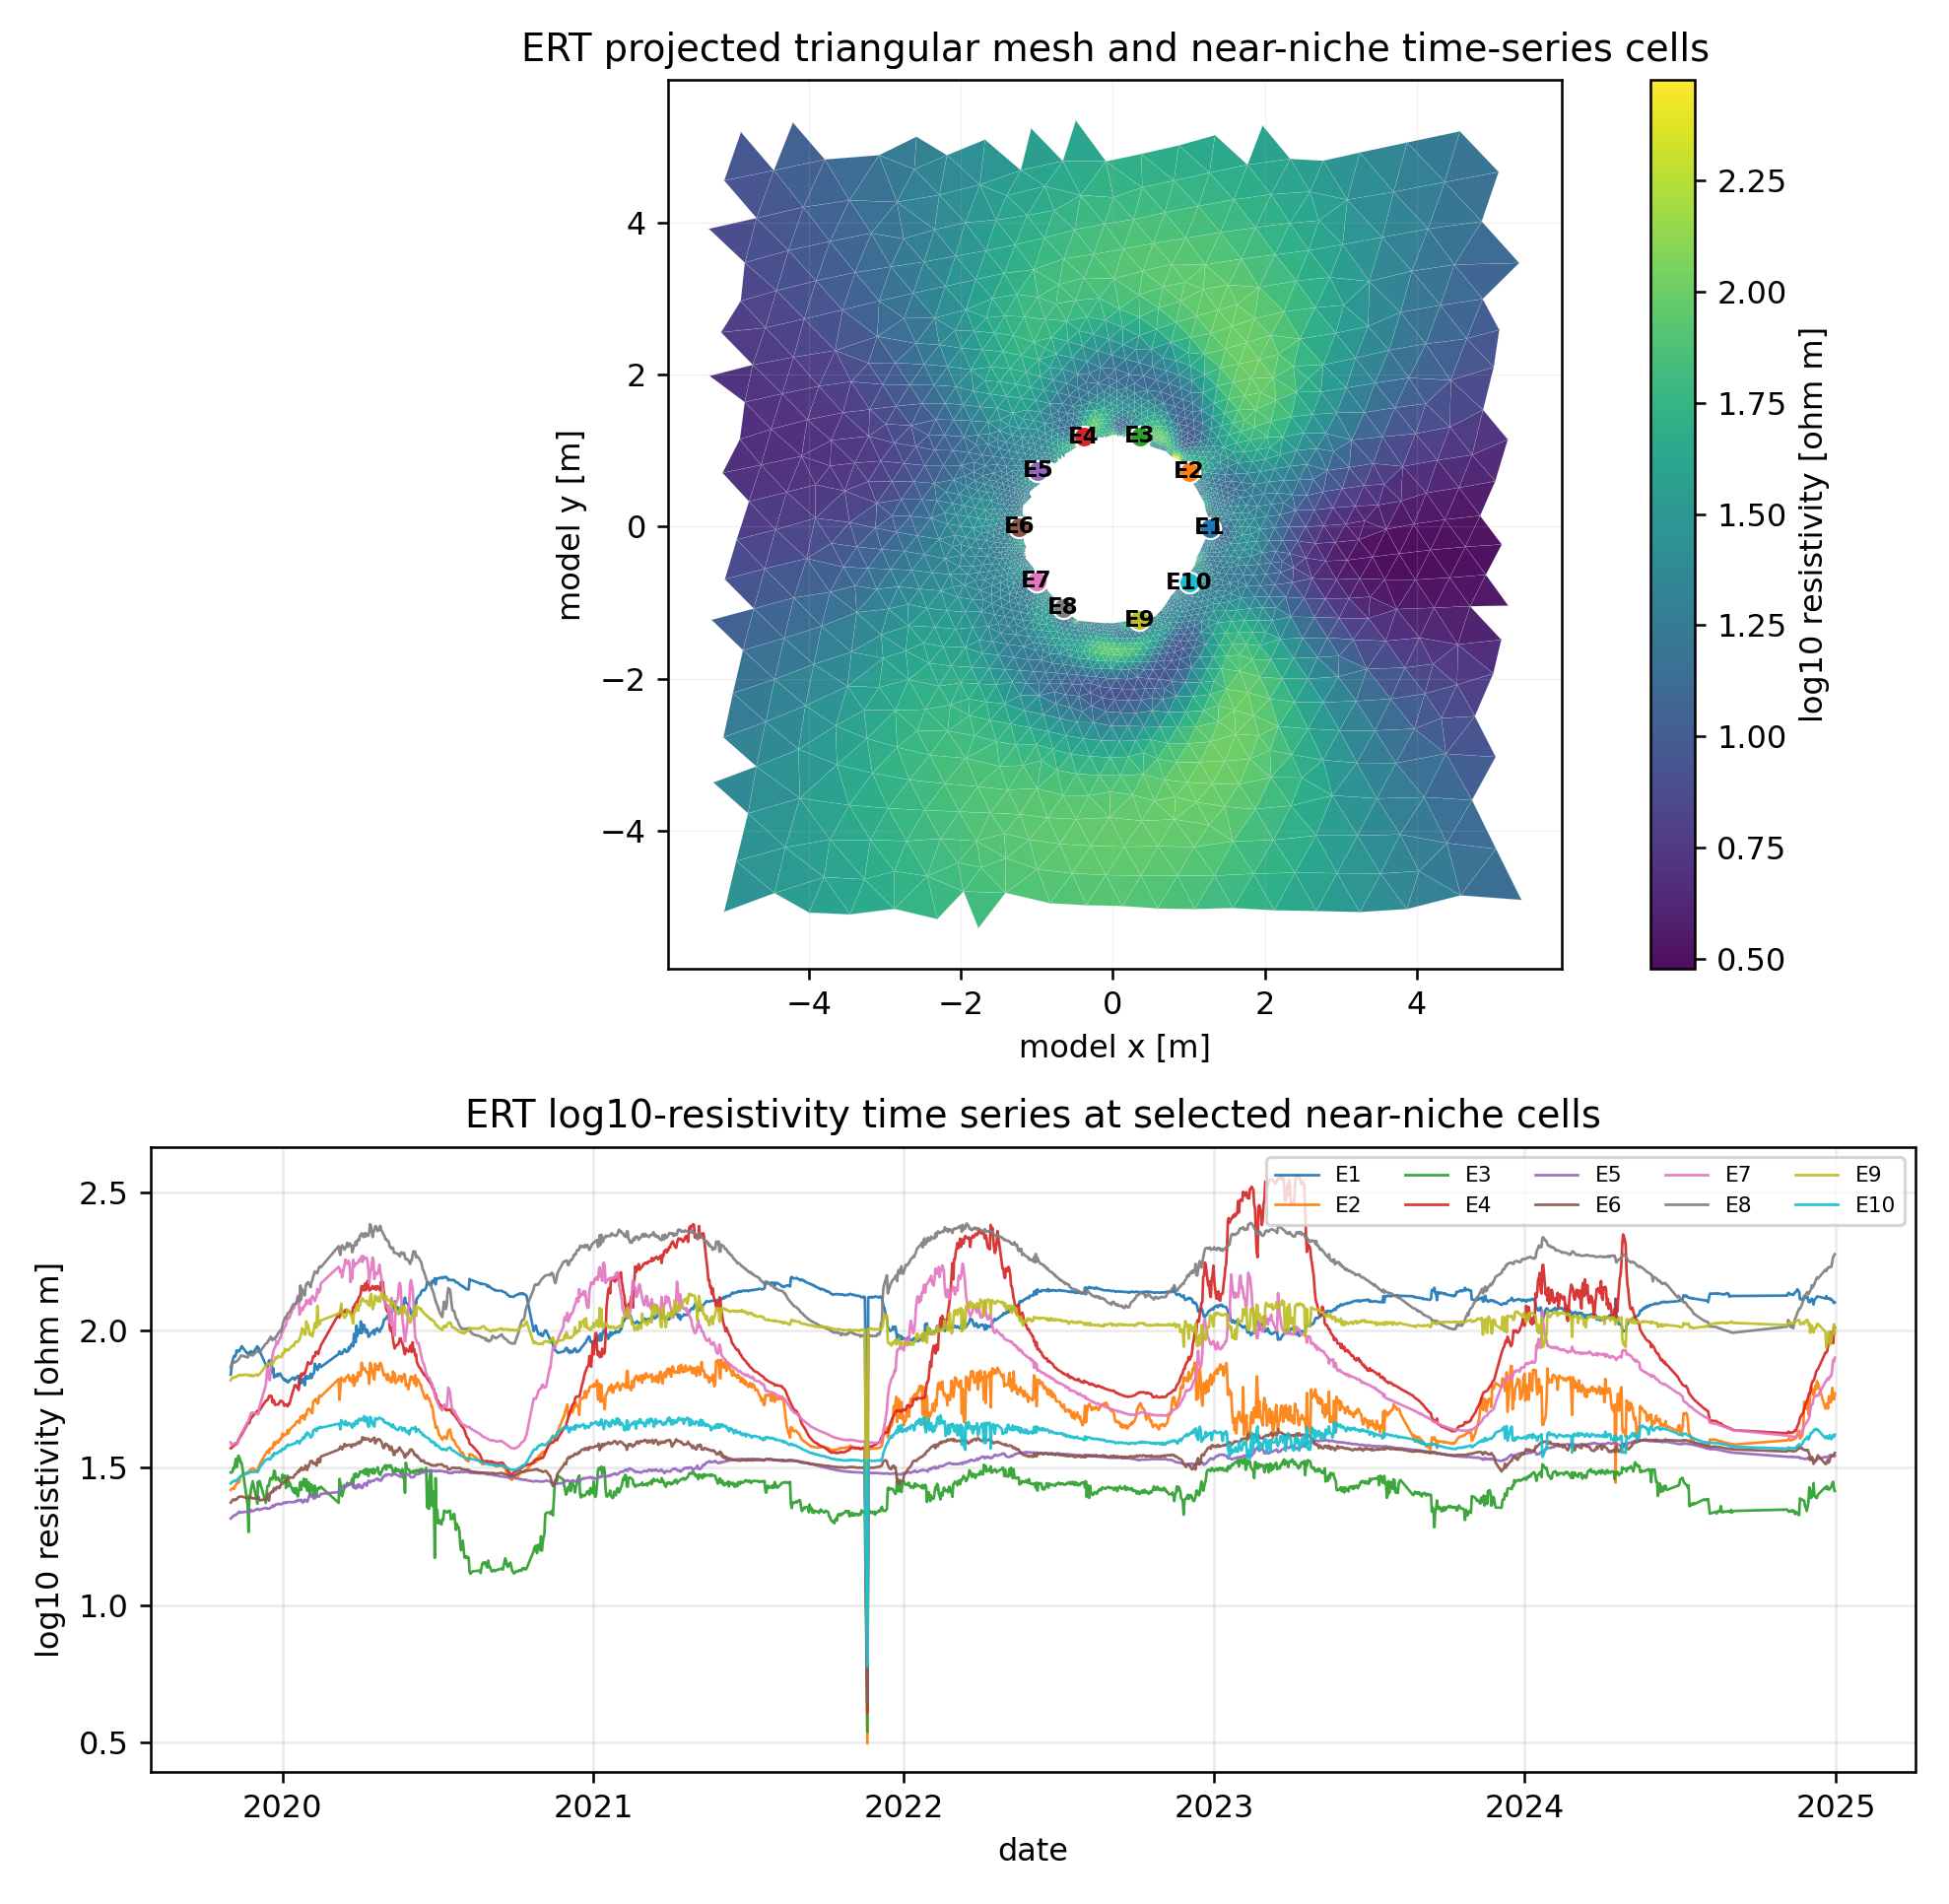
\includegraphics[width=0.98\textwidth]{figures/ert_data_visualisation.png}
\caption{ERT measured-data visualisation.  The upper panel shows the projected
triangular ERT mesh coloured by reference log10-resistivity in the model frame,
with ten near-niche cells marked as E1--E10.  These cells are selected from the
approximate 1.5 m centre-support subset, distributed by polar angle around the
niche and biased toward the shallow near-surface annulus.  The lower panel shows
their log10-resistivity histories over the matched ERT VTK timesteps.  The dense
spatial and temporal coverage makes ERT valuable for constraining desaturation
patterns, but the mesh cells are correlated inversion products and cannot be
treated as independent point observations.}
\label{fig:ert-data}
\end{figure}

\paragraph{Inversion incorporation.}
ERT should enter through a forward operator rather than directly in the PDE:
OGS computes \(\pp\) and \(\Sat\), the model converts \(\thetaw=\npor\Sat\) to a
bulk-resistivity prediction, and the ERT operator compares that prediction with the
projected resistivity image.  Spatially, the current transform places ERT cells in the
2D OGS frame and flags an approximate support ring; the exact tunnel/niche mask and
35 cm rock-depth convention are still provider-decision gates.  Temporally, each ERT
field should be matched to the corresponding OGS output date with an accepted
tolerance.  The residual belongs in \(\log_{10}\rho\) with a covariance or aggregation
model; until that covariance is available, ERT remains diagnostic and should not add
thousands of independent mesh-cell likelihood rows.

\subsection{Taupe/TDR Trend Candidate}

Taupe/TDR currently provides trend information:
\[
r_{\mathrm{Taupe,trend}} =
\widehat{\Delta\thetaw_{\mathrm{model}}} -
\widehat{\Delta T_{\mathrm{Taupe}}},
\]
where hats denote within-series robust standardization.  This avoids claiming the
workbook values are calibrated volumetric water-content percent or permittivity
before the Taupe unit/calibration gate closes.

The Taupe workbook notation used in the plots is as follows.  A3 and A4 are the
source workbook sheet/sensor labels for the mapped Taupe borehole supports
\(\code{BCD-A3}\) and \(\code{BCD-A4}\).  In the current 2D model coordinates,
A3 runs from \(\code{BCD-A3 Anfang}=(-1.170742,0.039013)\) to
\(\code{BCD-A3 Ende}=(-5.602376,-0.742404)\), and A4 runs from
\(\code{BCD-A4 Anfang}=(-0.020680,-1.108987)\) to
\(\code{BCD-A4 Ende}=(-0.020680,-5.508987)\).  The \(\code{Anfang}\) point is
the near-niche end of the Taupe support; the EDZ-band distances are measured from
that end into the rock along the support.  A3 and A4 are the two Taupe supports
that can be mapped to the current local OGS mesh.  A7 and A8 are retained in the
workbook/operator tables but are outside the current mesh support.

The labels \(\code{MV EDZ 0-10}\), \(\code{MV EDZ 10-20}\), \(\code{MV EDZ
20-30}\), \(\code{MV EDZ 30-40}\), and \(\code{MV EDZ 40-50}\) denote workbook
mean values over 10 cm EDZ bands measured from the niche wall along the Taupe
support.  Thus \(\code{0-10}\) means 0--10 cm from the wall, \(\code{10-20}\)
means 10--20 cm, and so on.  \(\code{MV EDZ 0-50}\) is the aggregate mean over
the whole 0--50 cm EDZ interval; it is not an additional independent depth band
separate from the five 10 cm bands.  These values are kept as Taupe workbook
proxy units until the provider confirms the absolute calibration.

\begin{figure}[H]
\centering
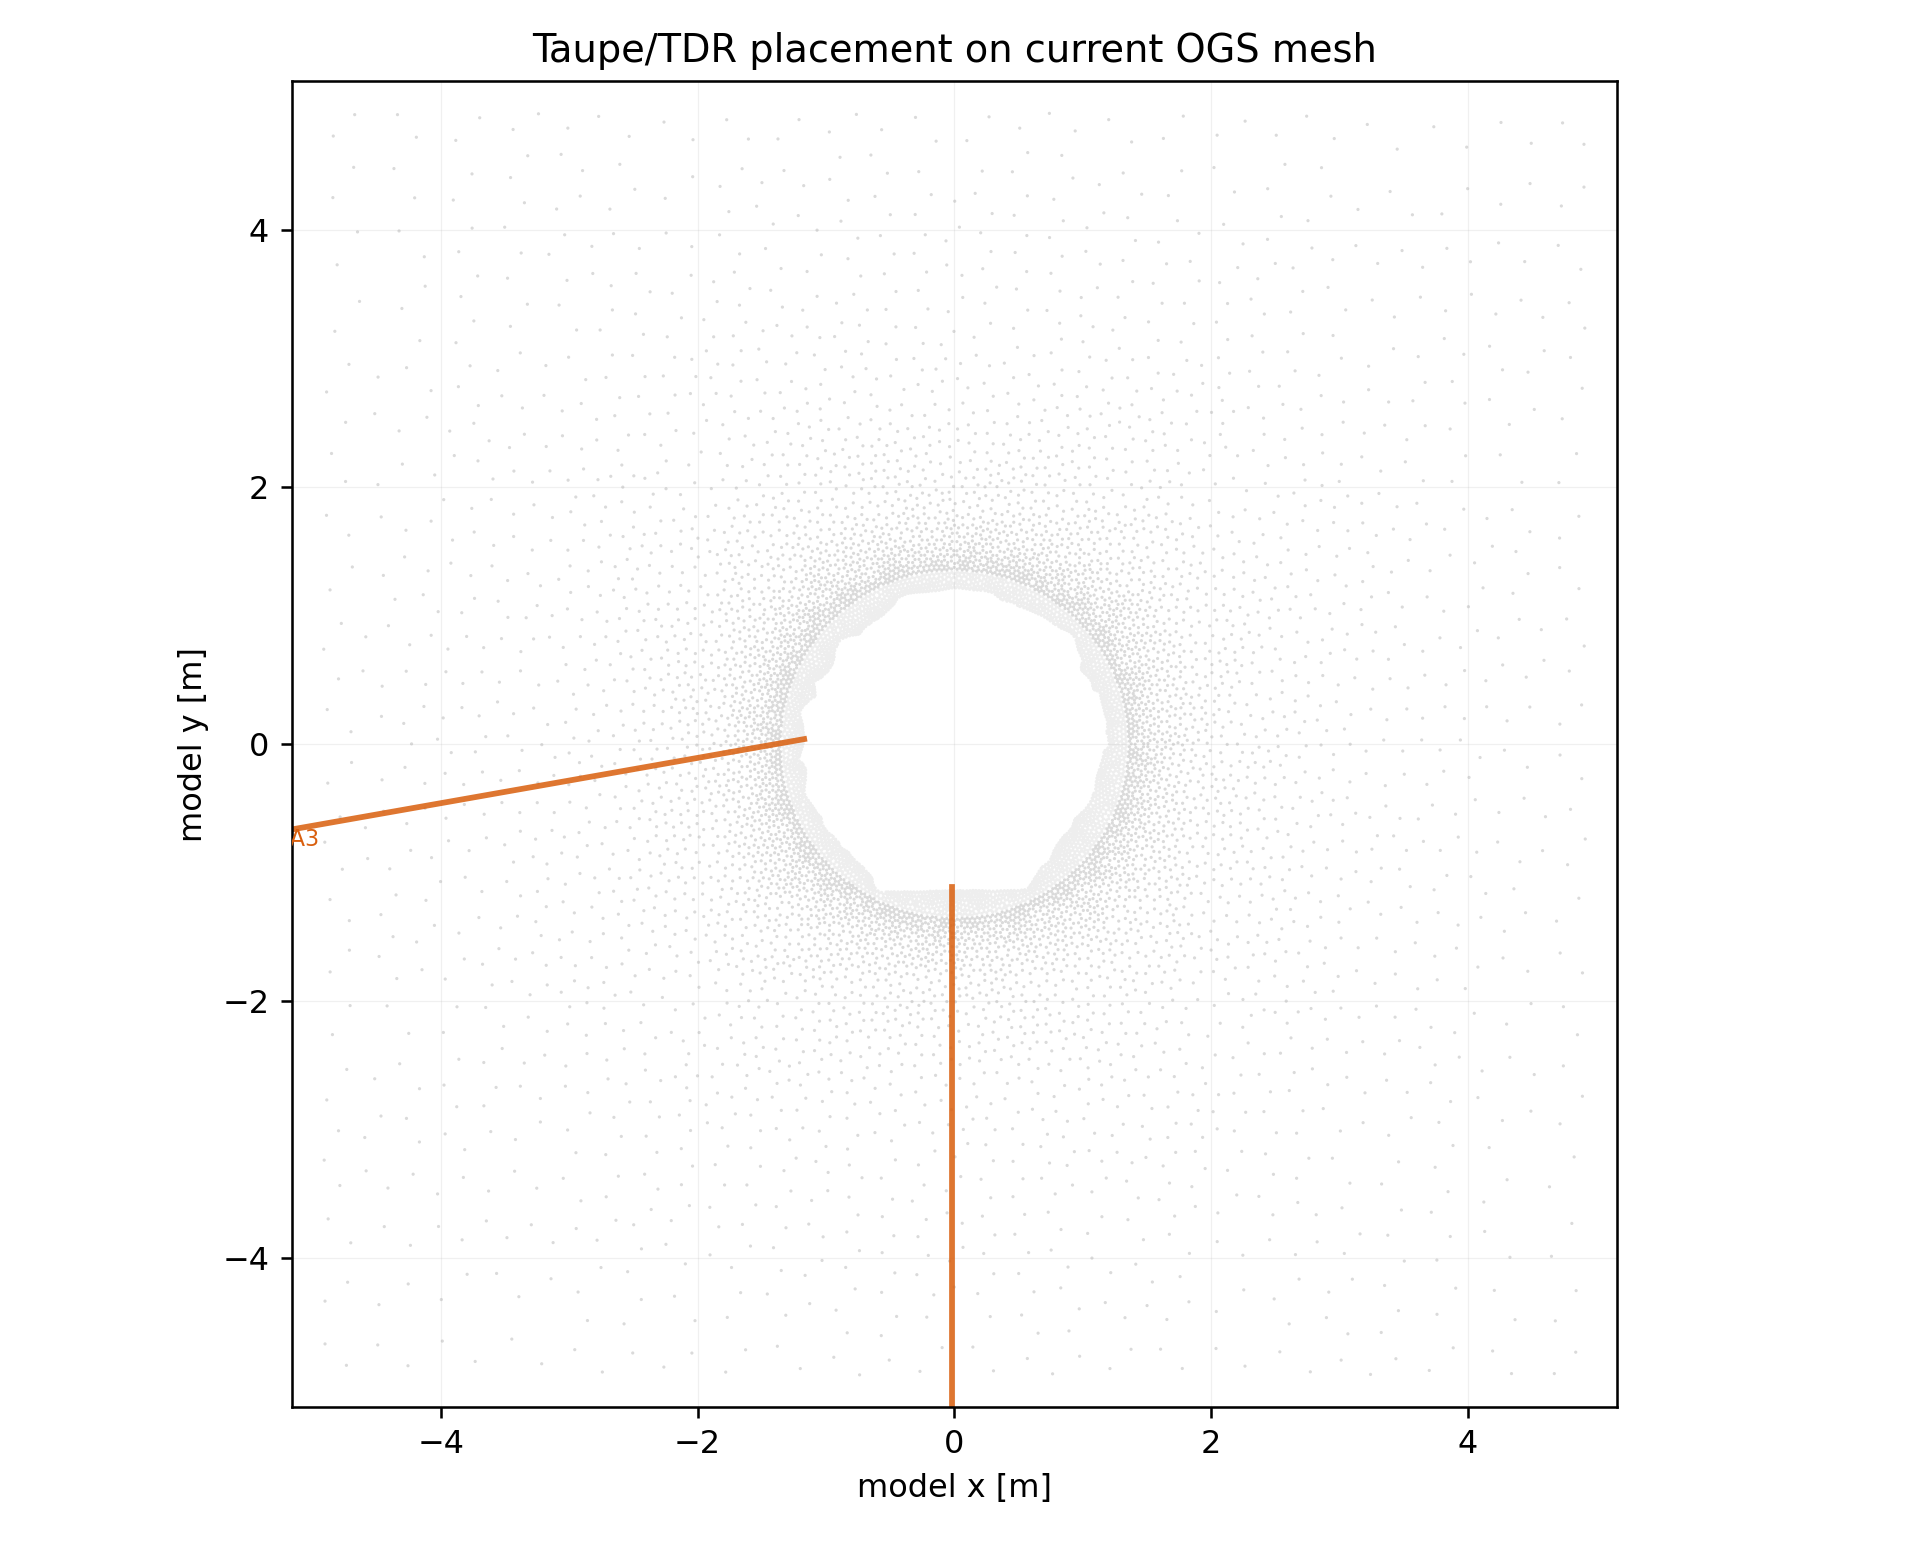
\includegraphics[width=0.86\textwidth]{figures/taupe_mesh_placement.png}
\caption{Taupe/TDR placement.  The mapped Taupe/TDR supports are plotted on the OGS
mesh as borehole-line supports.  A3 and A4 are usable for current Niche 4 trend
diagnostics; A7 and A8 provide workbook context but are outside the current mesh
support.}
\label{fig:taupe-placement}
\end{figure}

\begin{figure}[H]
\centering
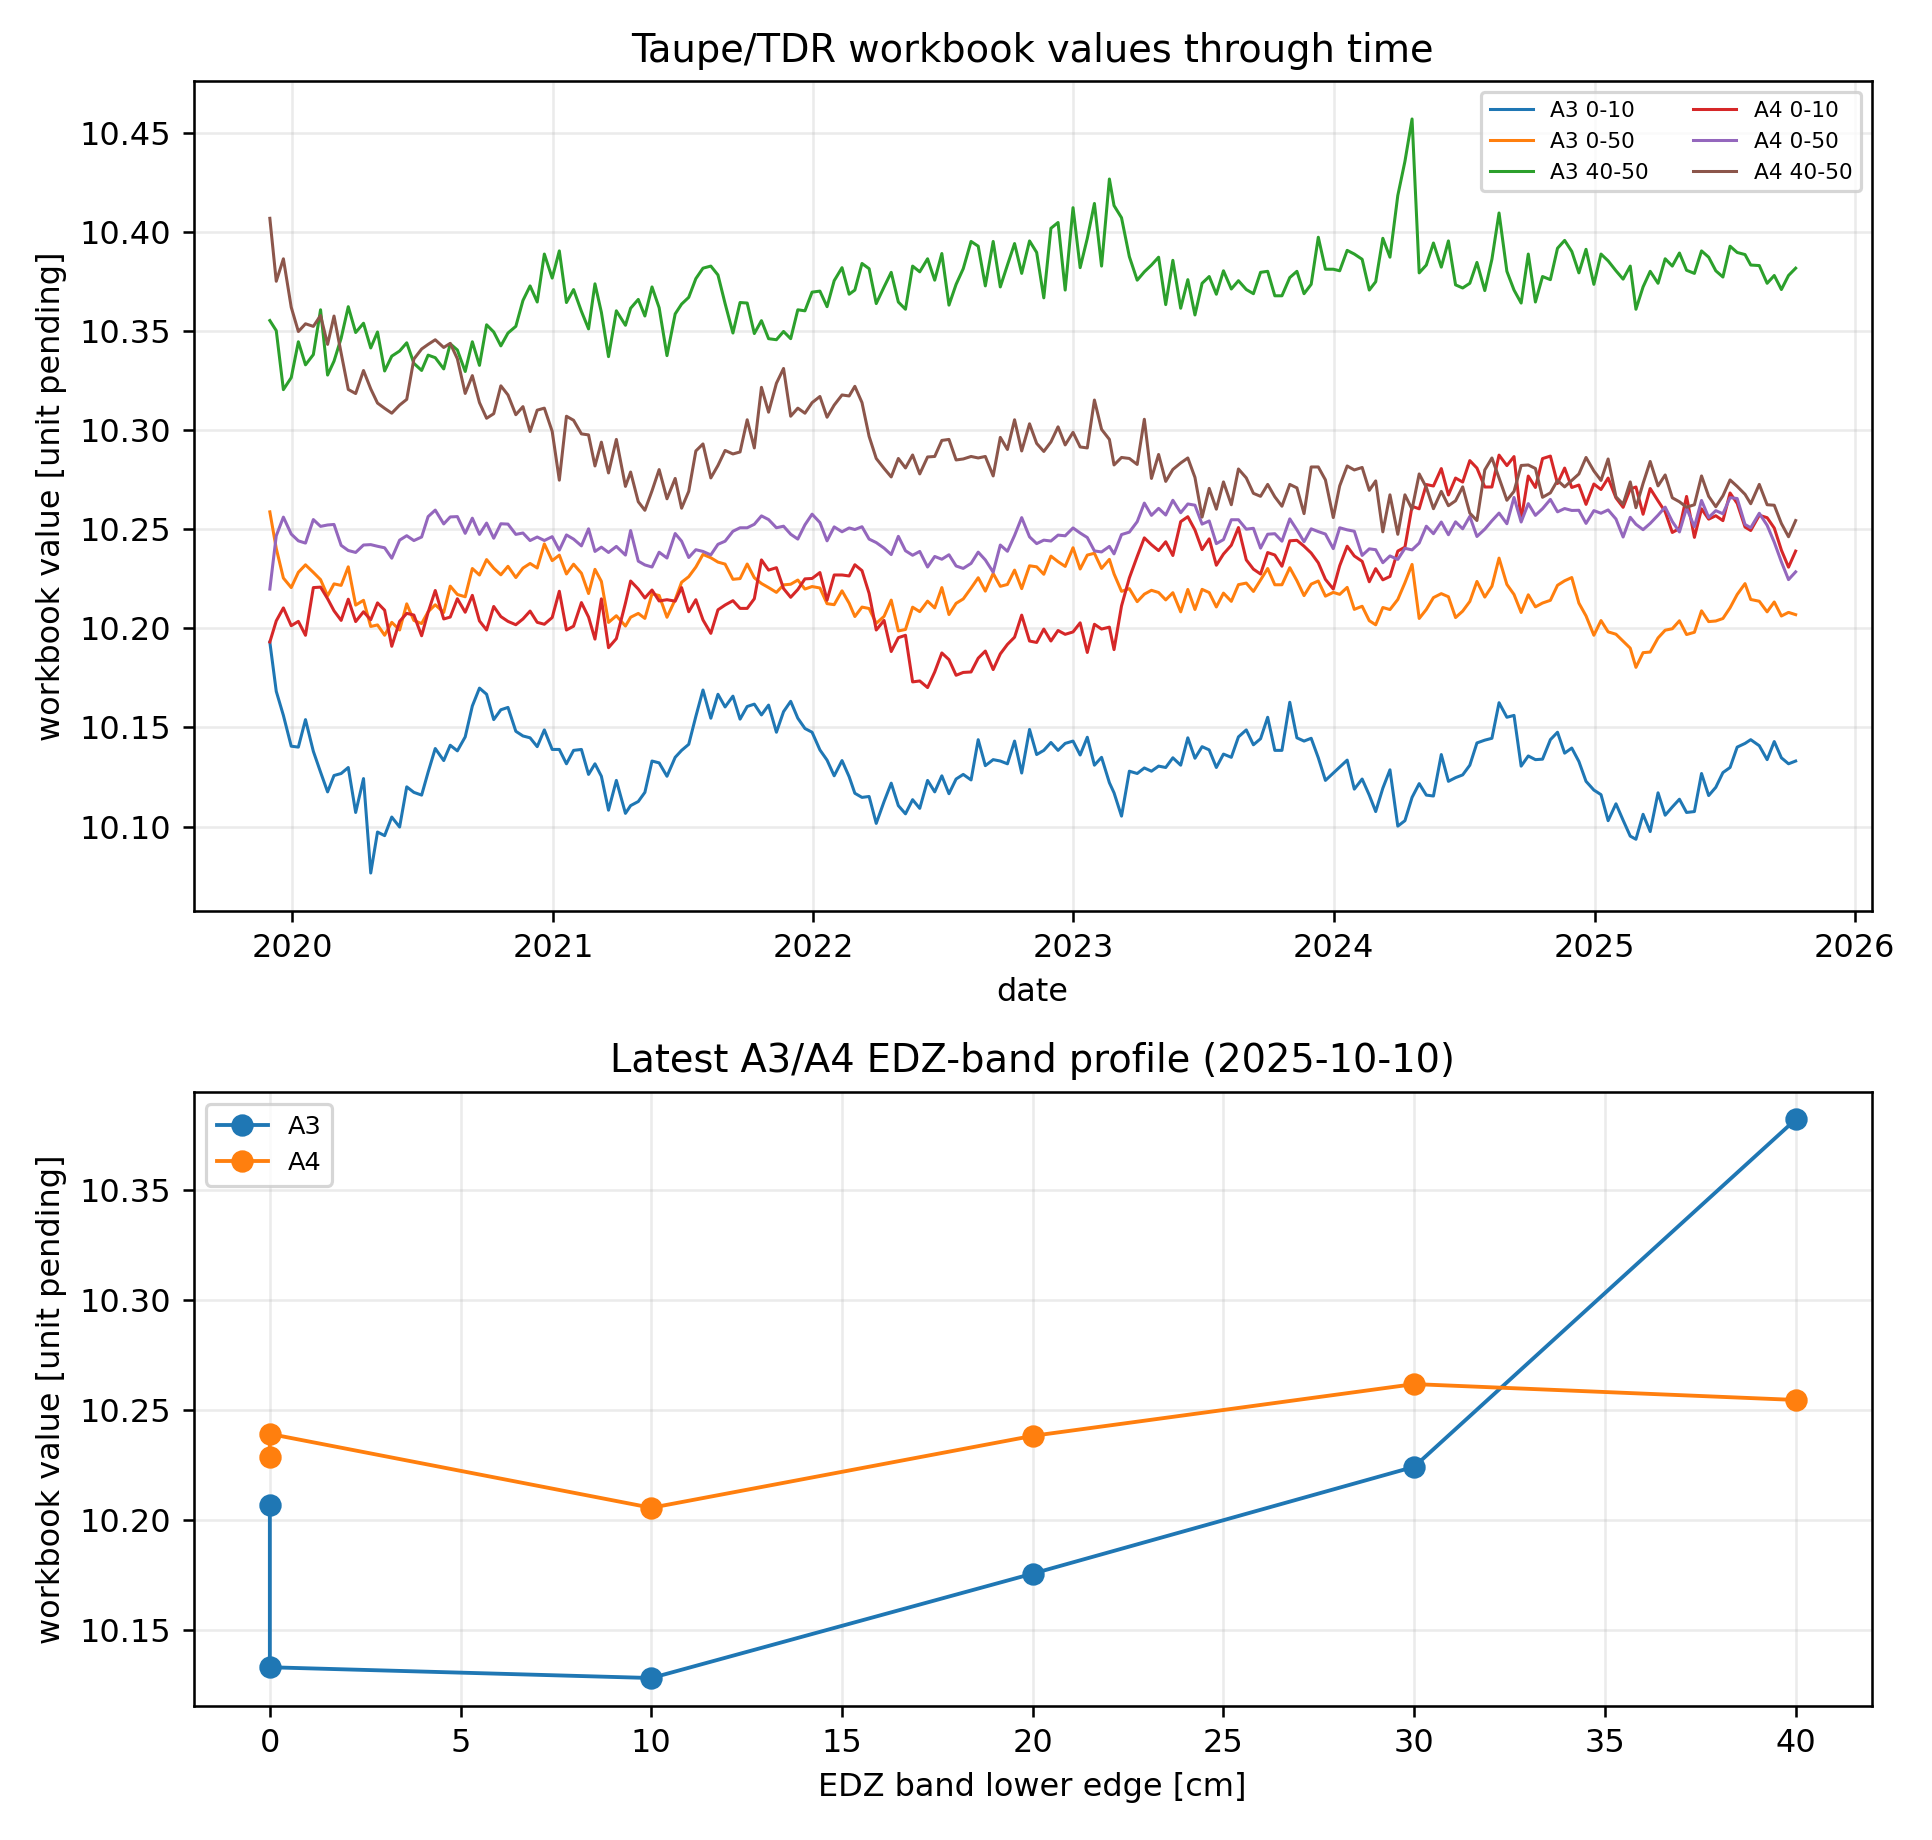
\includegraphics[width=0.98\textwidth]{figures/taupe_data_visualisation.png}
\caption{Taupe/TDR measured-data visualisation.  The upper panel shows representative
A3/A4 EDZ-band workbook values through time.  The lower panel shows the latest A3/A4
EDZ-band profile by distance from the niche wall.  Values are deliberately kept in
workbook units because the absolute unit and calibration equation remain unresolved.}
\label{fig:taupe-data}
\end{figure}

\paragraph{Inversion incorporation.}
Taupe/TDR would connect to the hydraulic state through \(\thetaw=\npor\Sat\), or
through a dielectric/water-content calibration if the provider supplies one.  Spatially,
the operator should average OGS \(\theta\) over EDZ bands along the mapped Taupe
borehole supports, with A3/A4 active for the present mesh and A7/A8 excluded unless a
larger support model is introduced.  Temporally, workbook dates can be matched to OGS
output dates from 2019 to 2025.  The current safe residual is a standardized trend or
anomaly residual by sensor and EDZ band; an absolute residual should wait for the
Taupe unit, calibration, uncertainty, and baseline convention.

\subsection{RH Boundary Candidate}

The Kelvin relation maps RH to capillary pressure or liquid pressure:
\[
\pcap \approx -\frac{\rho_\ell R T}{M_w}\ln(\mathrm{RH}),
\qquad
\pp \approx -\pcap
\]
under the gauge convention used here.  The current local conversion assumes
\(T=298.15\) K and \(\rho_\ell=1095\,\mathrm{kg\,m^{-3}}\).  Because the active OGS
curve differs strongly from the local RH5/RH6-derived curves, RH should remain a
boundary provenance audit until the original curve source, filtering, time zero, and
extension policy are confirmed.

\begin{figure}[H]
\centering
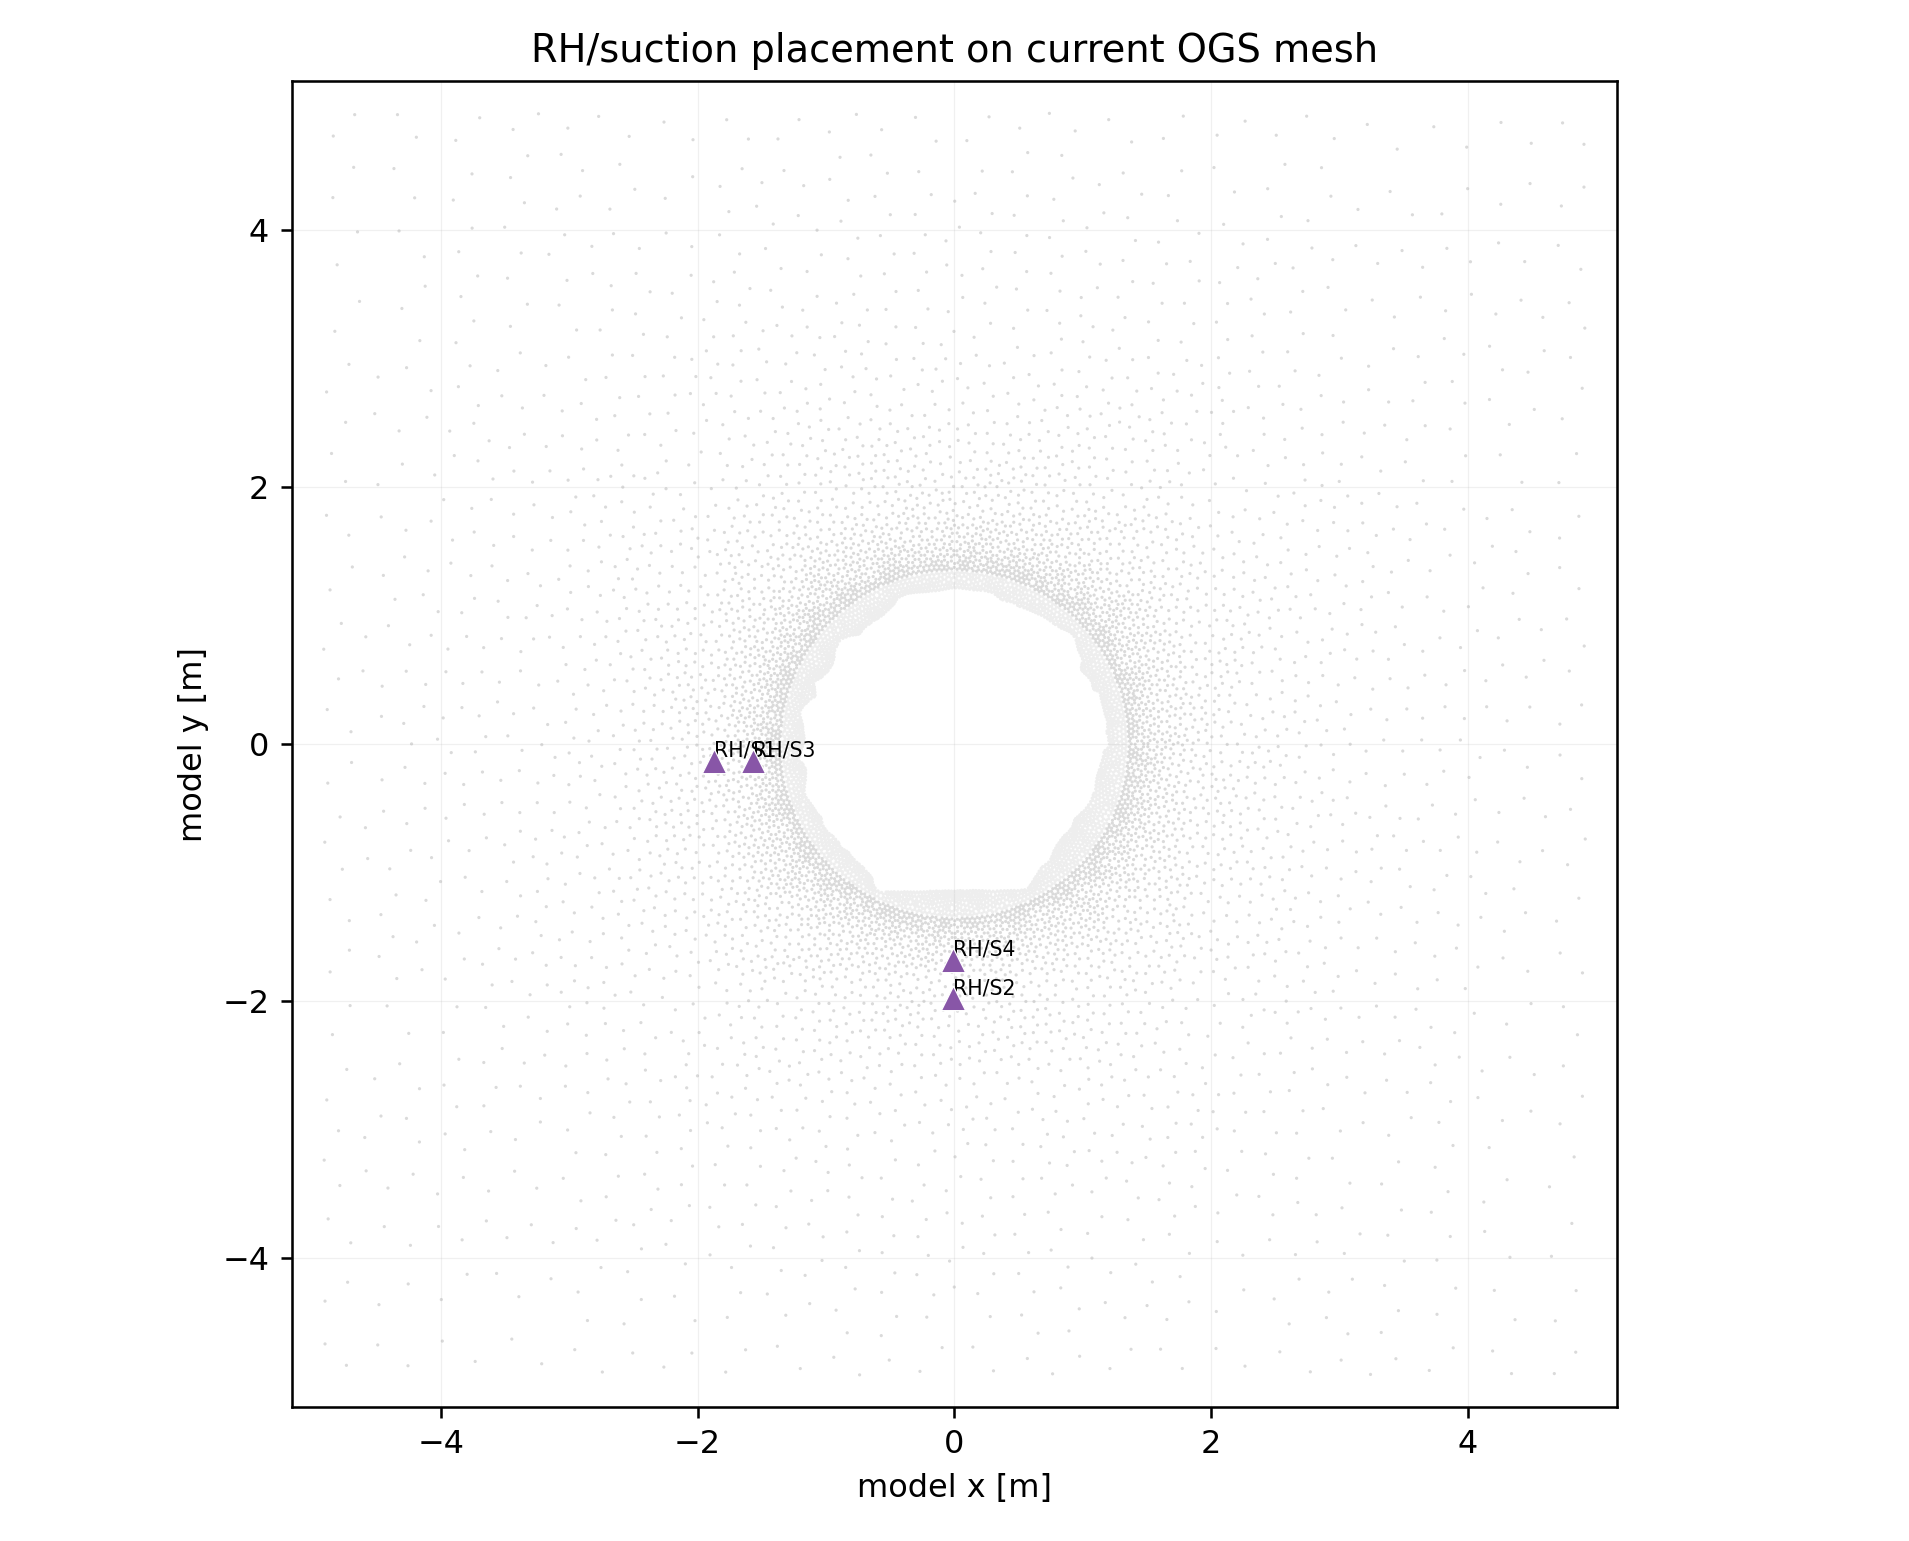
\includegraphics[width=0.86\textwidth]{figures/rh_mesh_placement.png}
\caption{RH/suction placement.  The plotted points are the currently mapped RH or
suction coordinate rows in the same OGS 2D model frame used for the boundary audit.
They identify the near-niche support for evaluating whether the active open-niche
pressure boundary curve is consistent with the humidity-derived suction signal.}
\label{fig:rh-placement}
\end{figure}

\begin{figure}[H]
\centering
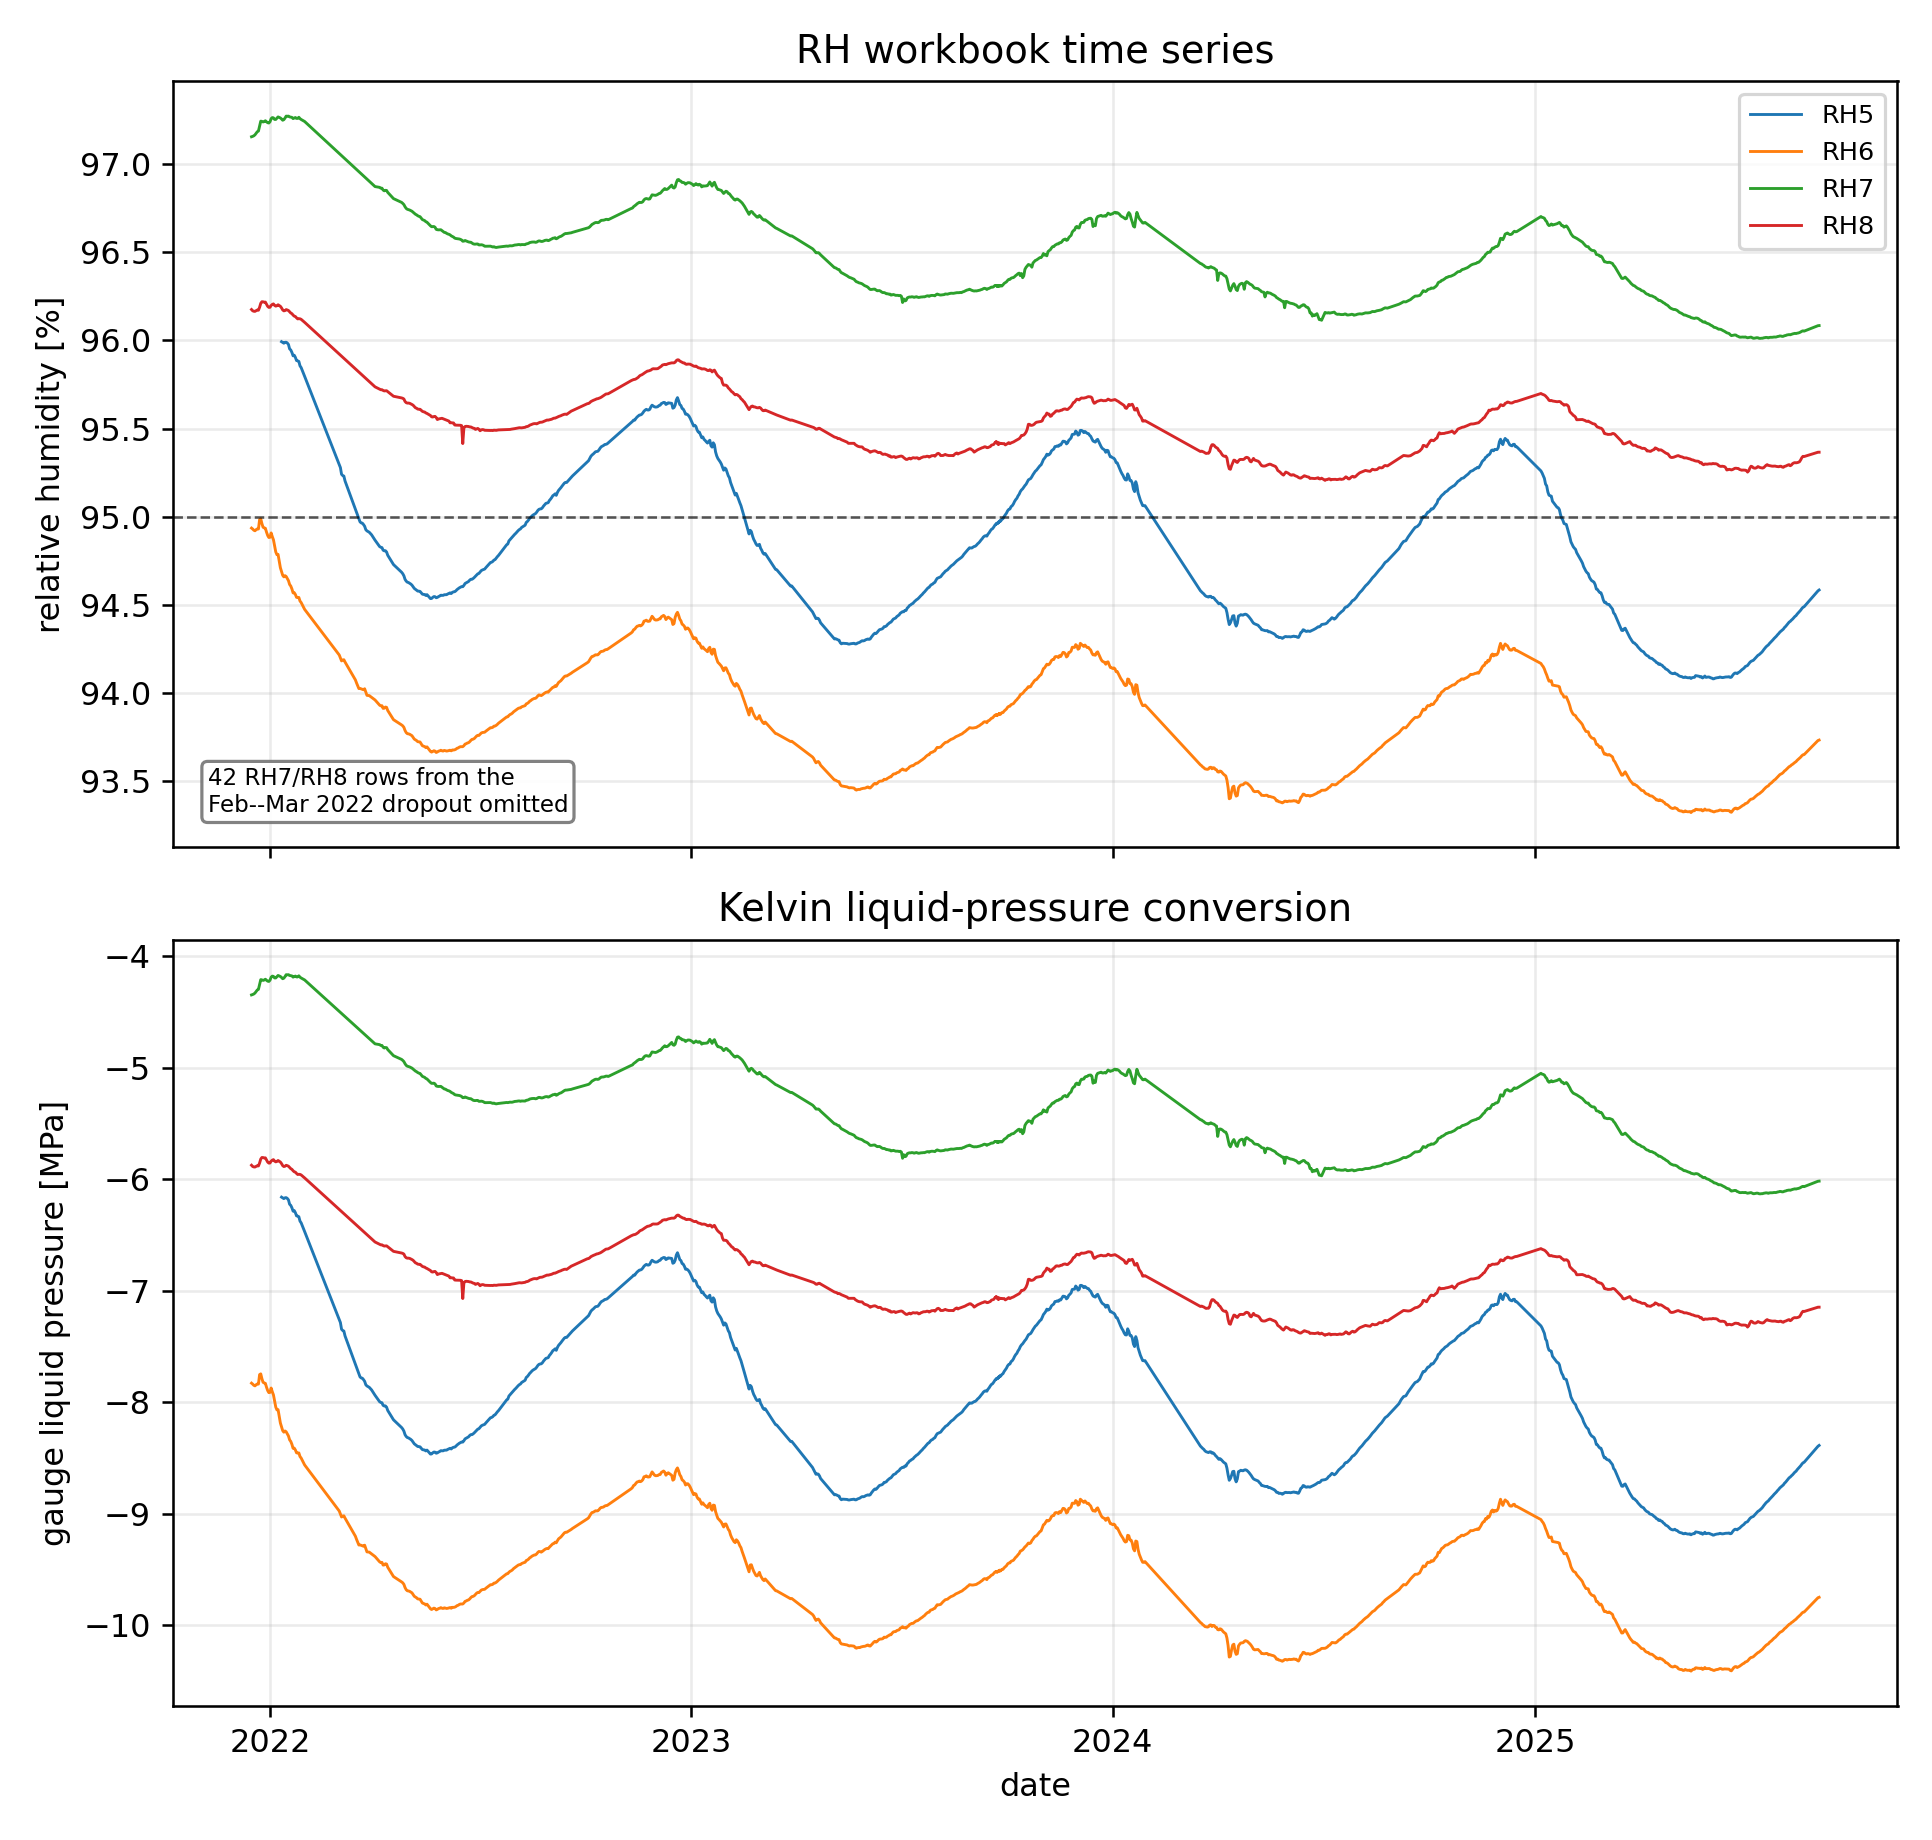
\includegraphics[width=0.98\textwidth]{figures/rh_data_visualisation.png}
\caption{RH/suction measured-data visualisation.  The upper panel shows RH5--RH8
relative humidity through time after omitting the RH7/RH8 dropout episode from
2022-02-28 to 2022-03-30, treated here as corrupted logger/sensor values.  The
lower panel shows the corresponding Kelvin-equation gauge liquid-pressure
conversion in MPa using the stated constants, with the same rows omitted.  These
converted pressures are boundary-forcing evidence, not yet a replacement for the
active OGS curve.}
\label{fig:rh-data}
\end{figure}

\paragraph{Inversion incorporation.}
RH enters the model through the pressure boundary and retention relation, not as a
direct interior material measurement.  In the PDE it constrains \(\pp(t)\) on the
open-niche boundary and can later inform \(p_b\), \(m\), or boundary-pressure
uncertainty in the van Genuchten saturation law.  Spatially, the mapped RH/suction
points are near-boundary audit supports rather than volume averages.  Temporally, the
daily RH values should be converted with a documented Kelvin convention and compared
against the model boundary curve over the same time window.  Until sensor screening,
time zero, constants, smoothing, and extension policy are agreed, RH remains a
boundary audit and scenario generator rather than a hard likelihood term.

\subsection{Other-HM Monitoring Candidate}

The other-HM material is useful, but it is not yet a mesh-ready residual package.
The position plots below use the extracted source visualisation \(x/z\) frame from
the HM layout.  That frame is deliberately not treated as the current OGS 2D model
frame.  For inversion, every HM stream still needs numeric values, timestamps,
support geometry, units, sign/reference convention, and uncertainty before a hard
likelihood can be assigned.

\begin{longtable}{@{}L{0.16\textwidth}L{0.19\textwidth}L{0.23\textwidth}Y@{}}
\caption{How each other-HM measurement type would enter an inversion once numeric
exports and support metadata are supplied.}\\
\toprule
Measurement type & PDE/model field & Spatial and temporal operator & Current inversion status \\
\midrule
\endfirsthead
\toprule
Measurement type & PDE/model field & Spatial and temporal operator & Current inversion status \\
\midrule
\endhead
\bottomrule
\endlastfoot
Mini-piezometer & Liquid pressure \(\pp\), or hydraulic head derived from \(\pp\). & Sample \(\pp(\bm x,t)\) at BCD-A28--BCD-A31 sensor supports after coordinates, elevation/reference pressure, and gauge/absolute convention are confirmed.  Match to sensor timestamps. & High-priority pressure residual candidate, blocked until Geoscope numeric exports and quality flags are supplied. \\
Extensometer & Displacement \(\uu\), strain, or relative displacement over a gauge length. & Project OGS displacement onto the instrument axis over each anchor/gauge support; compare only over valid periods, excluding failed BCD-A9/B10 periods after September 2025. & Mechanical validation residual candidate, blocked by missing time series, sign convention, support, and failure metadata. \\
Crackmeter or fracture aperture & Relative displacement \(\Delta\uu\) across a crack plane, or aperture change. & Compute local displacement difference across the mapped crackmeter support with a defined positive-opening sign and zero date. & Qualitative open/closed-niche deformation gate for now; hard residual blocked by missing crackmeter numeric exports and unique support positions. \\
Laser scan & Surface displacement or scan-difference field derived from \(\uu\). & Register OGS surface displacement to the scan frame and compare masked surface-difference statistics at each survey epoch. & Medium-priority mechanical plausibility gate, blocked by missing statistical interpretation, registration uncertainty, and survey masks. \\
Miniprisma geodesy & 3D displacement \(\uu\). & Sample or project displacement at each prism location, with 3D-to-2D reduction explicitly defined if the current 2D model is used. & Position support exists in the source frame; numeric campaign series and covariance are needed for likelihood use. \\
Convergence points & Relative displacement between tunnel/niche points. & Compare distance or component changes between paired points through time, using the same reference epoch as the survey. & Support context only until numeric convergence histories and uncertainties are available. \\
Precision levelling & Vertical displacement component of \(\uu\). & Compare model vertical displacement at levelling points between the initial campaign and later survey epochs, using the survey reference frame and covariance. & Only a 12-point slide summary is available; this can check sign and order of magnitude, not support a calibrated residual. \\
Evapometer or climate proxy & Boundary flux or atmospheric forcing context. & Use as a boundary-condition audit for open-niche drying, not as an interior residual. & Context-only unless a documented flux/evaporation time series and boundary mapping are supplied. \\
\end{longtable}

\begin{figure}[H]
\centering
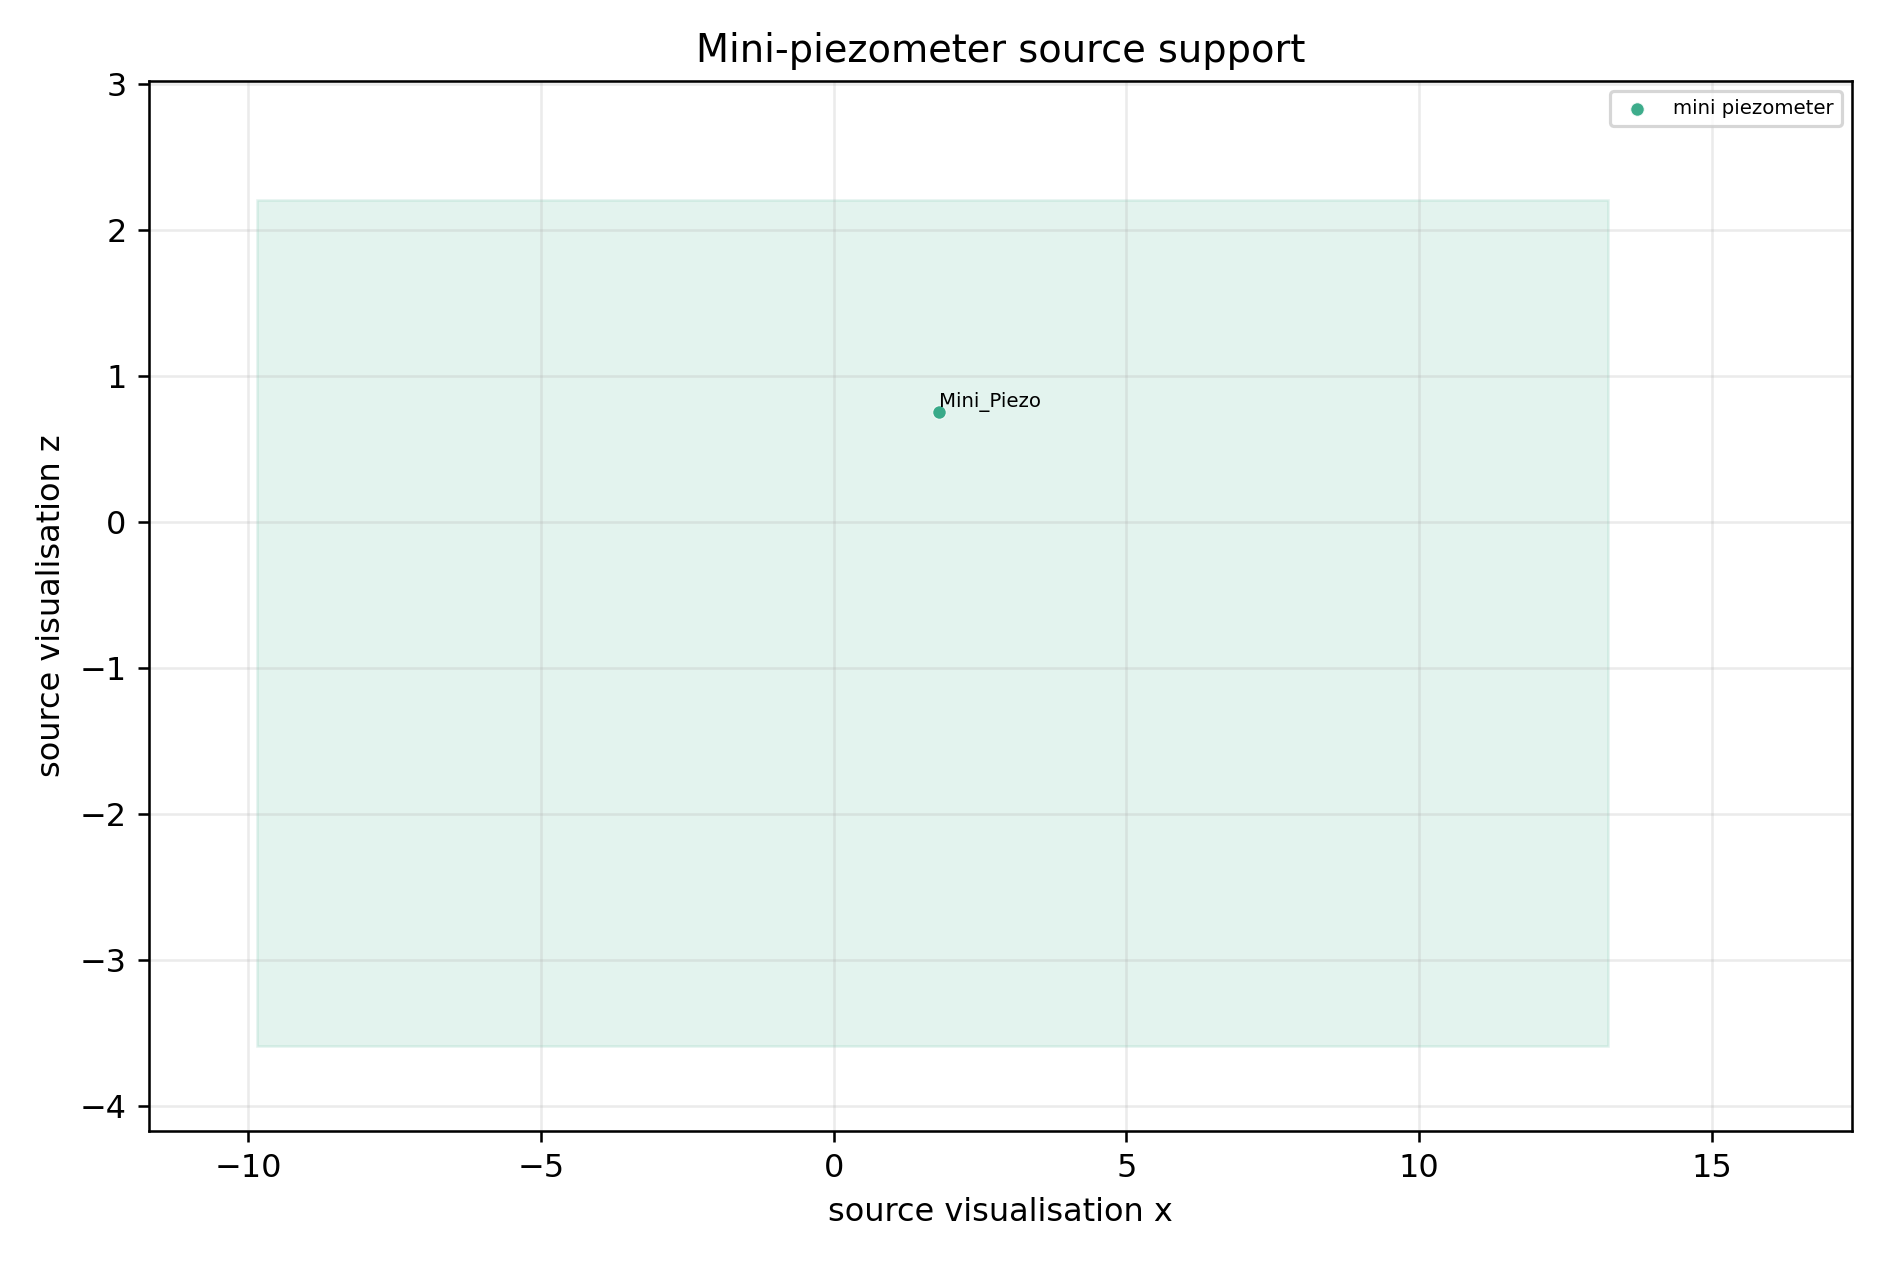
\includegraphics[width=0.95\textwidth]{figures/hm_mini_piezometer_positions.png}
\caption{Mini-piezometer source support.  The source layout contains one aggregated
Mini\_Piezo support zone; separate BCD-A28--BCD-A31 pressure residuals require the
Geoscope numeric export with individual sensor coordinates, reference convention, and
quality flags.}
\label{fig:hm-mini-piezo}
\end{figure}

\begin{figure}[H]
\centering
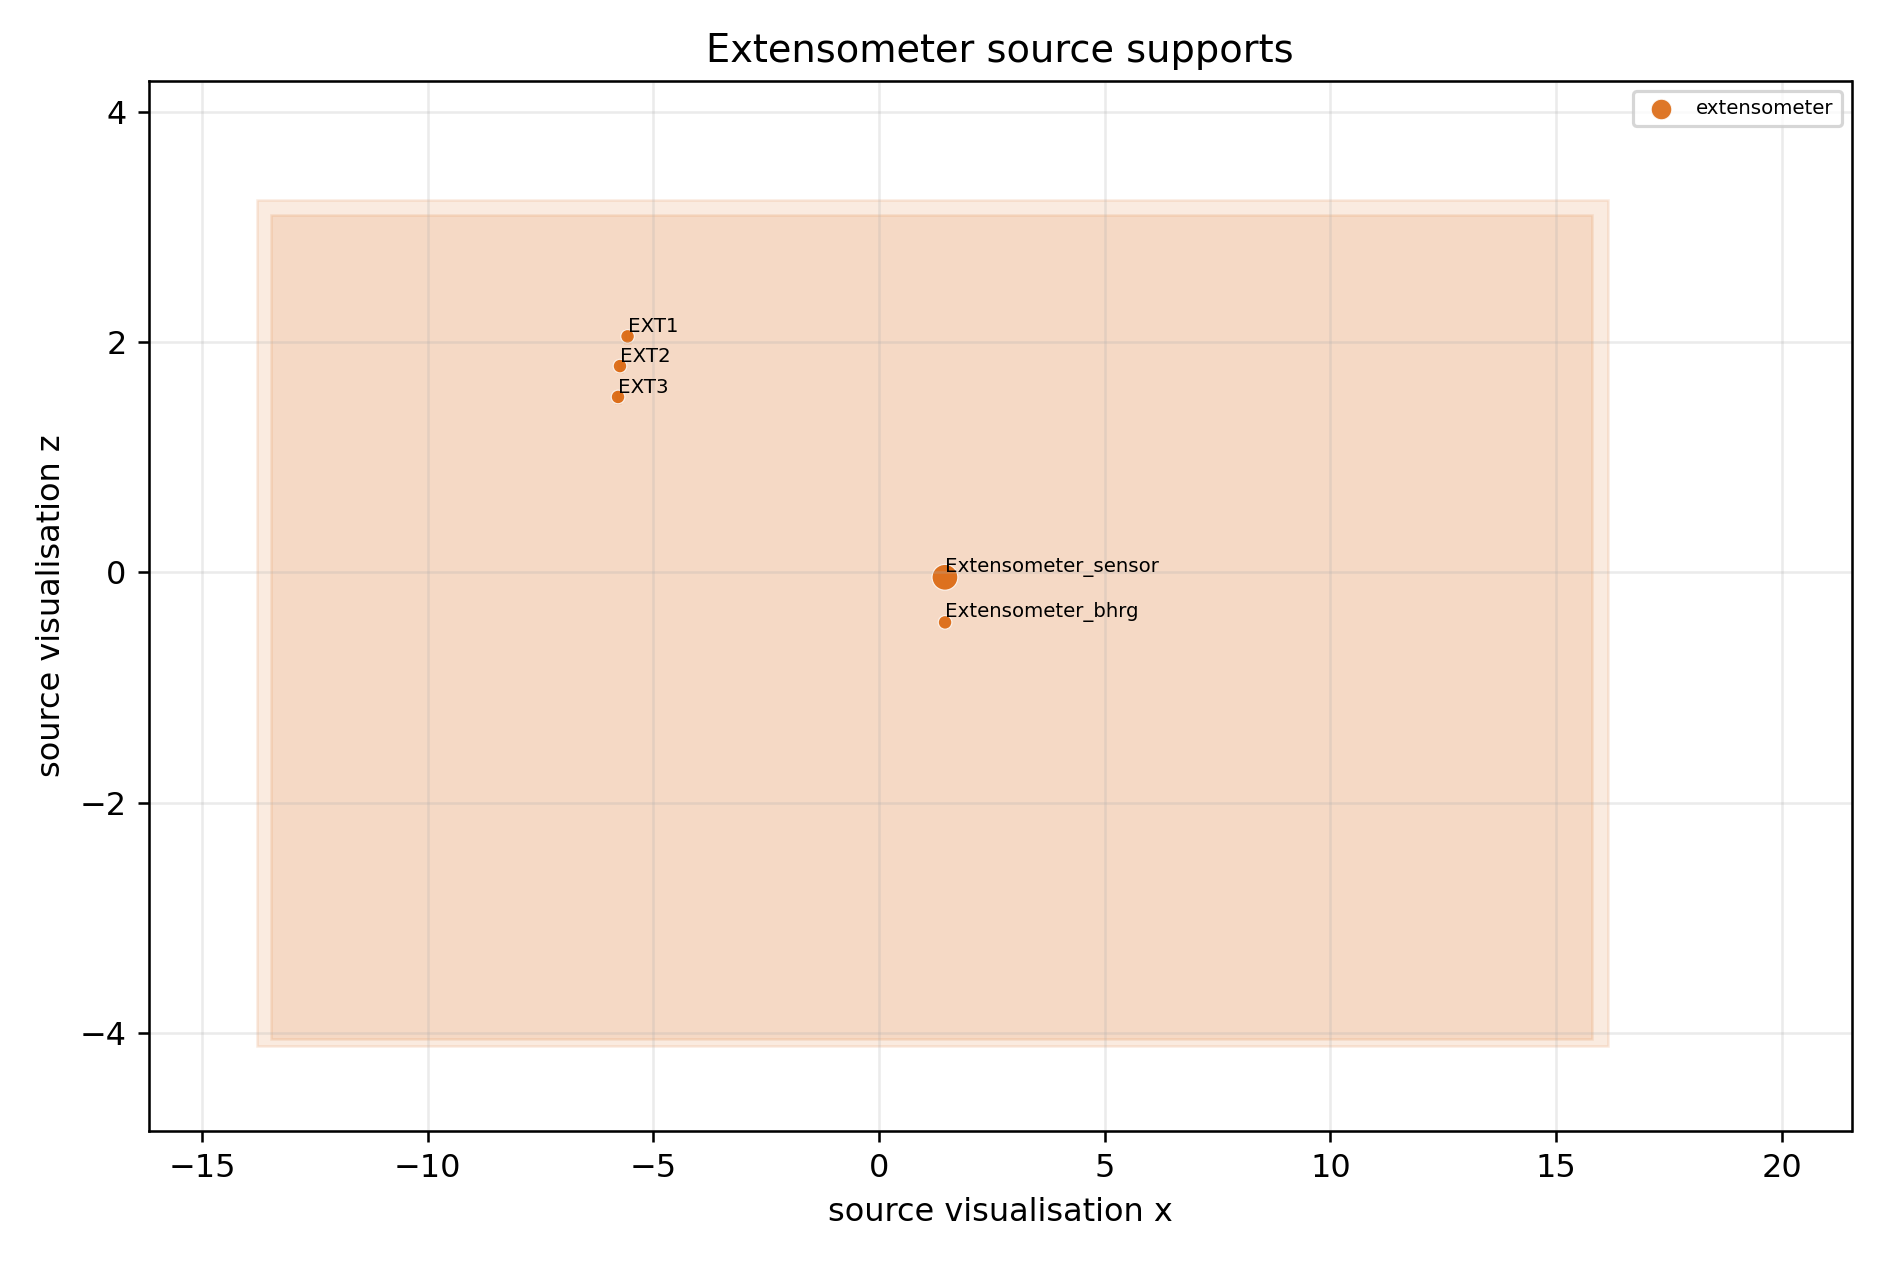
\includegraphics[width=0.95\textwidth]{figures/hm_extensometer_positions.png}
\caption{Extensometer source supports.  The plotted zones separate the broad
extensometer borehole/sensor supports from EXT1--EXT3 source positions.  These would
map to OGS displacement or strain only after anchor geometry, gauge length, sign
convention, and valid time ranges are provided.}
\label{fig:hm-extensometer}
\end{figure}

\begin{figure}[H]
\centering
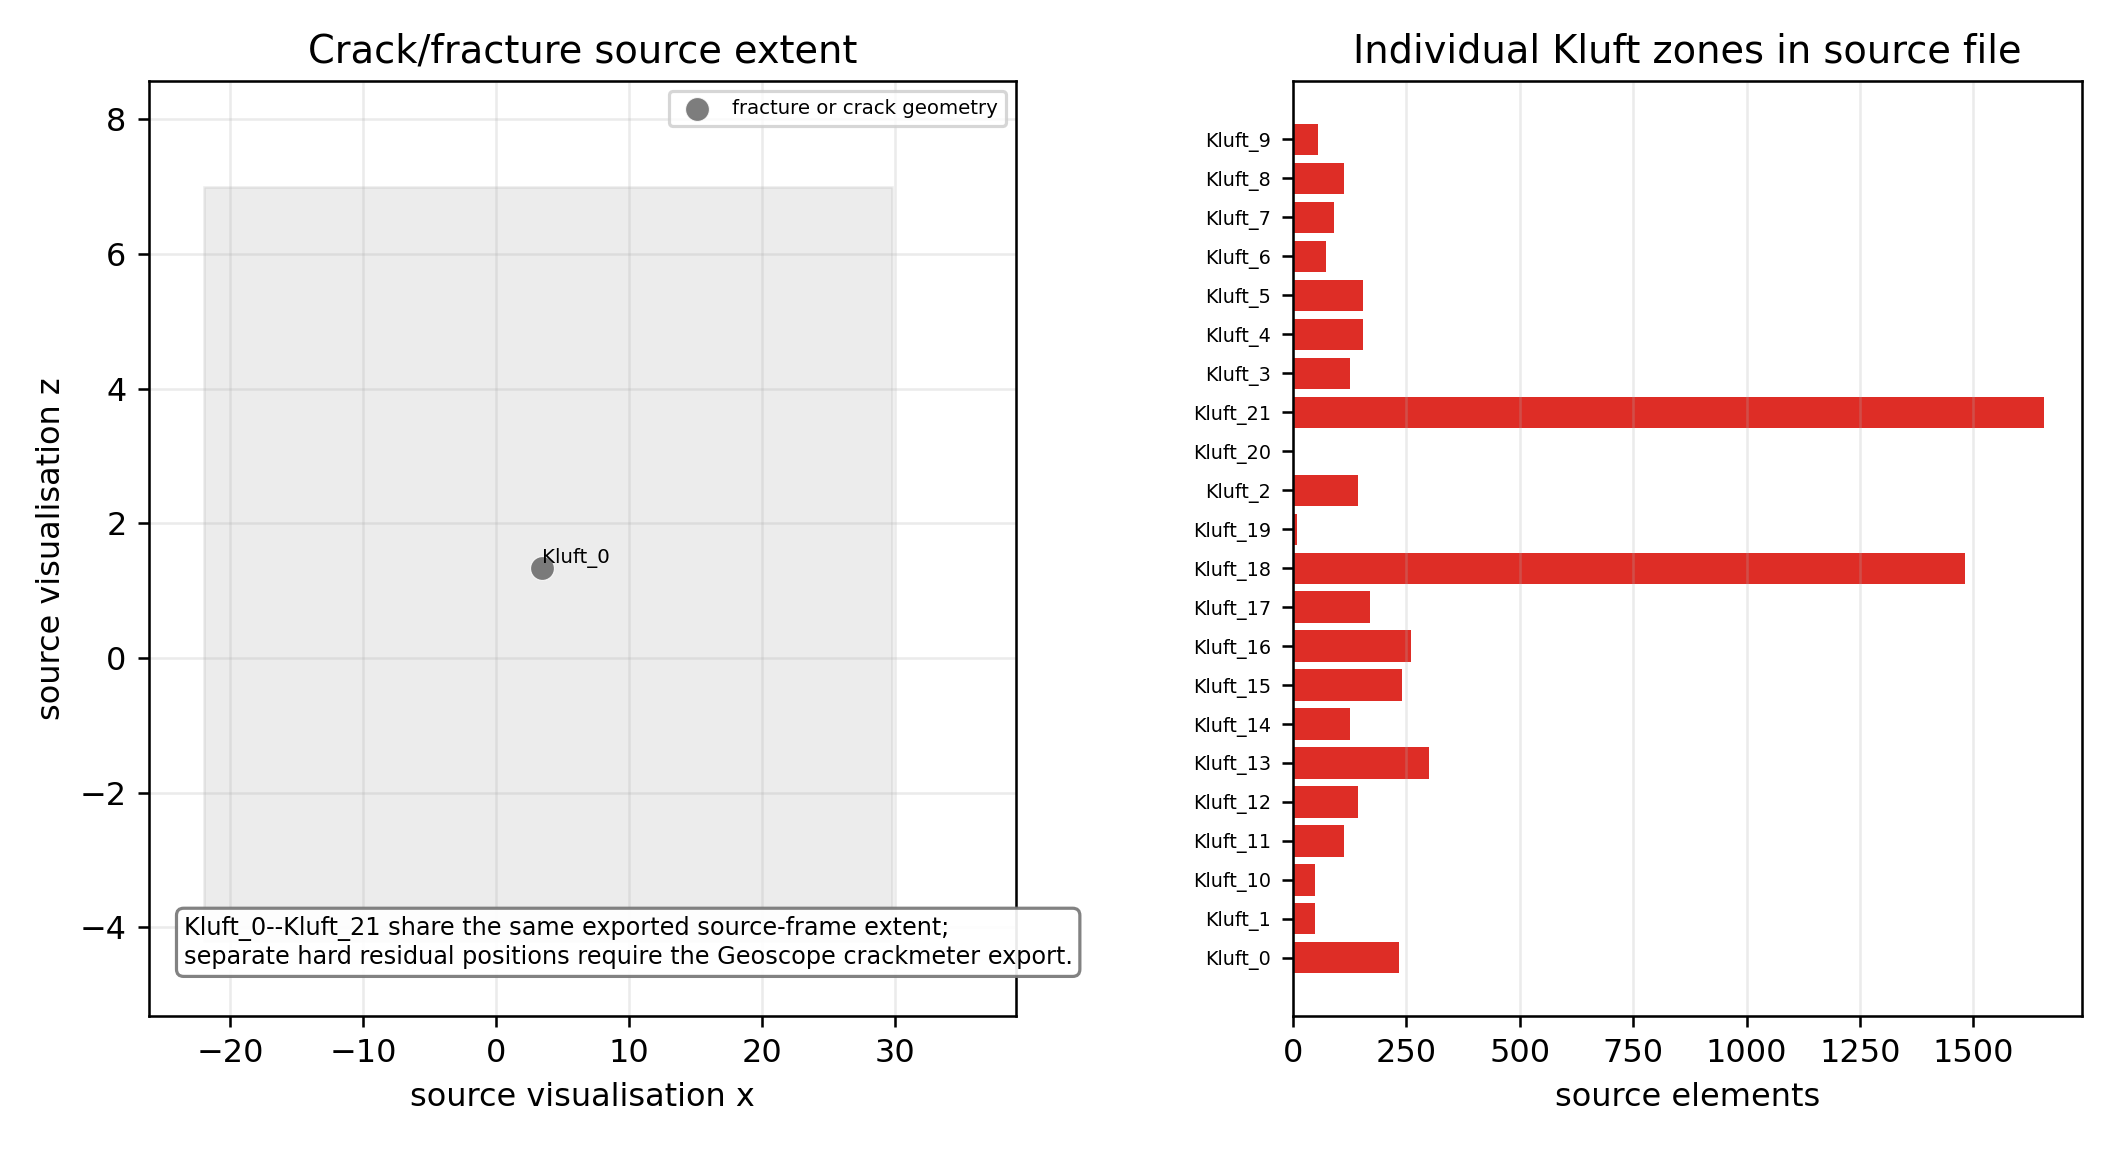
\includegraphics[width=0.98\textwidth]{figures/hm_crackmeter_positions.png}
\caption{Crack/fracture or crackmeter support information.  The left panel shows the
single exported source-frame extent shared by Kluft\_0--Kluft\_21.  The right panel
lists each Kluft zone separately by source-element count.  This documents the
available crack/fracture catalogue but also shows why unique crackmeter residual
positions still require the numeric Geoscope export.}
\label{fig:hm-crackmeter}
\end{figure}

\begin{figure}[H]
\centering
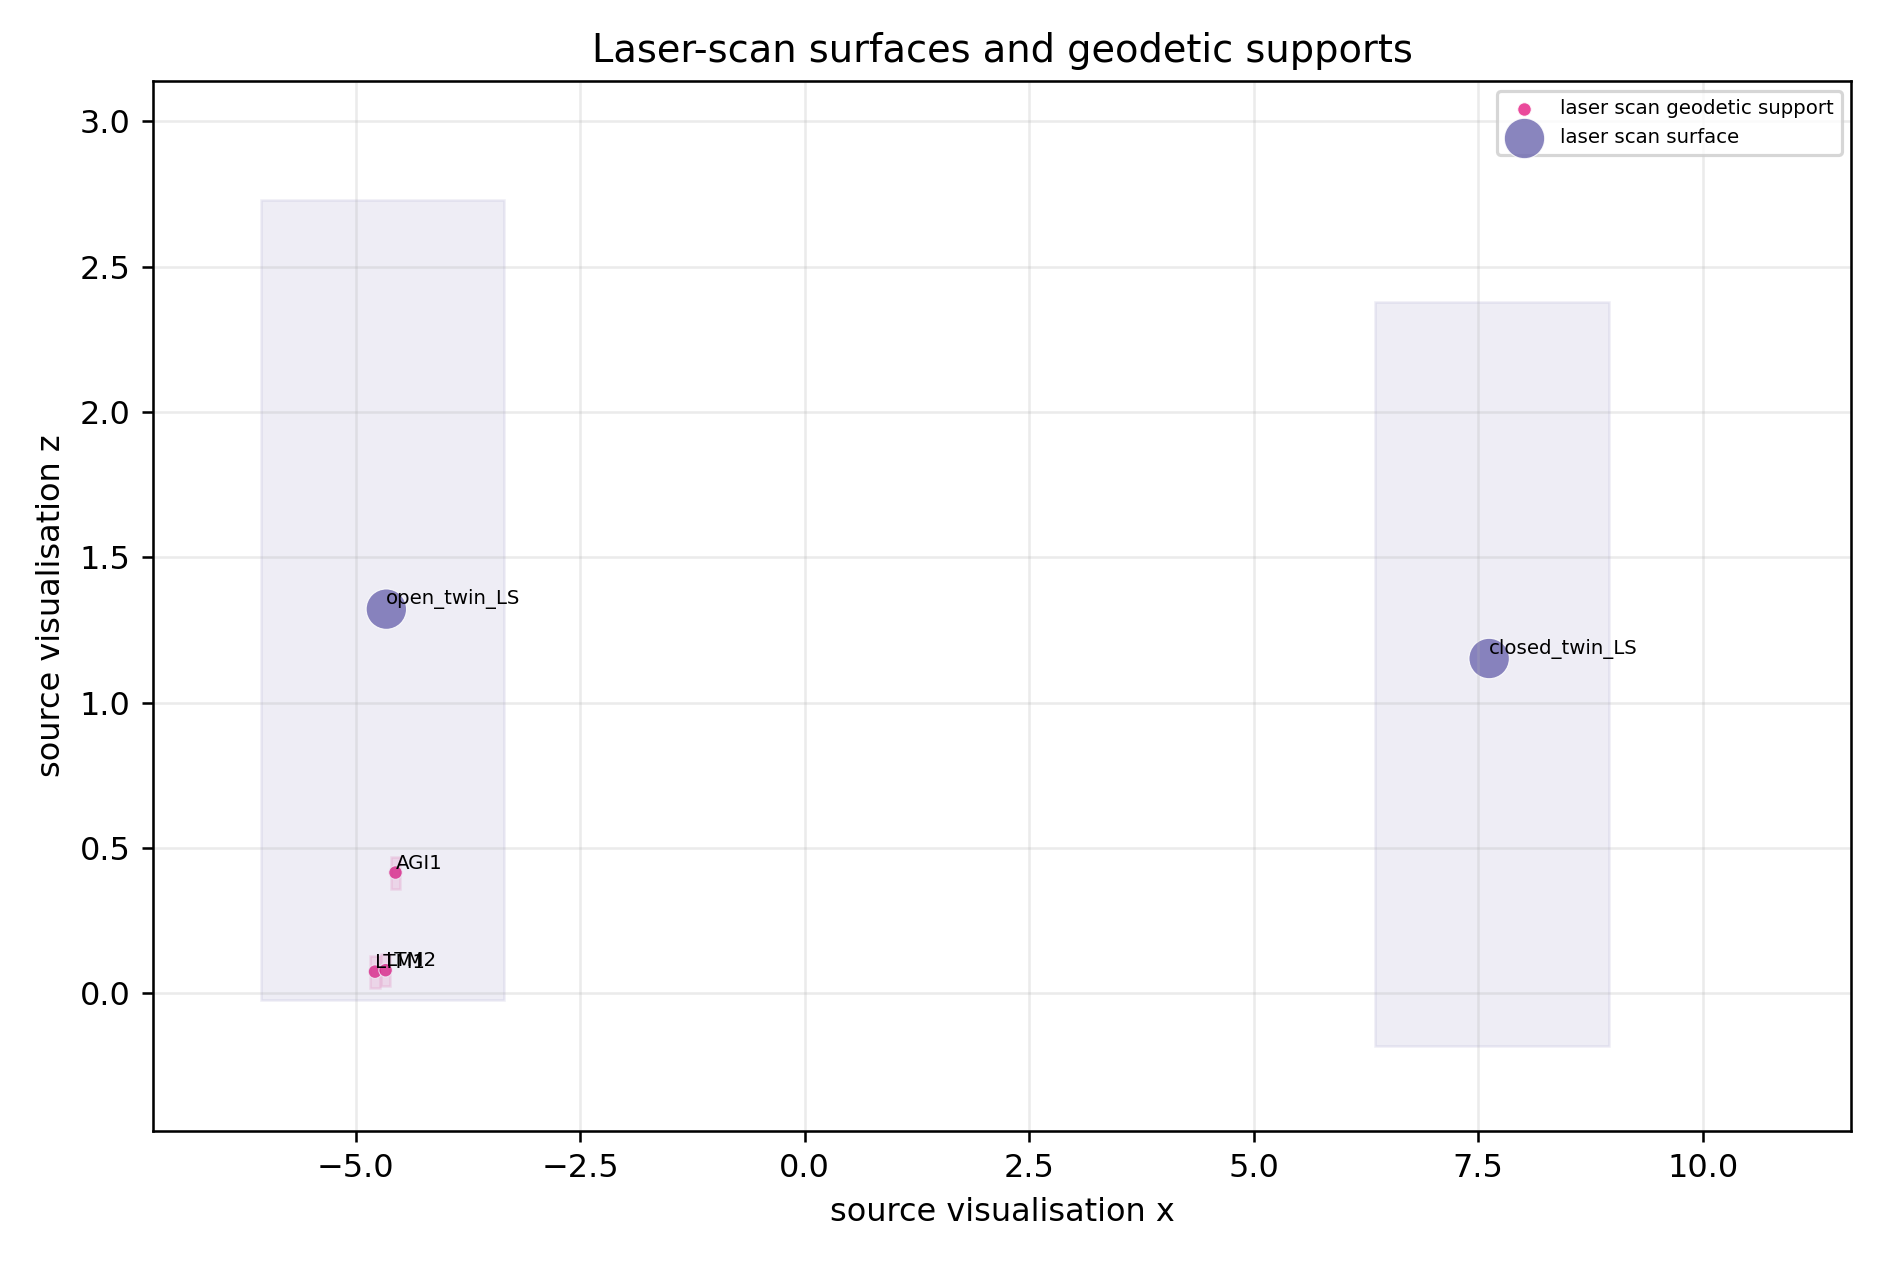
\includegraphics[width=0.95\textwidth]{figures/hm_laser_scan_positions.png}
\caption{Laser-scan and geodetic support positions in the source frame.  The two
large zones are the open- and closed-twin laser-scan surfaces; LTM1, LTM2, and AGI1
are geodetic support targets.  For inversion these would become surface-displacement
or scan-difference comparisons only after registration and uncertainty metadata are
known.}
\label{fig:hm-laser}
\end{figure}

\begin{figure}[H]
\centering
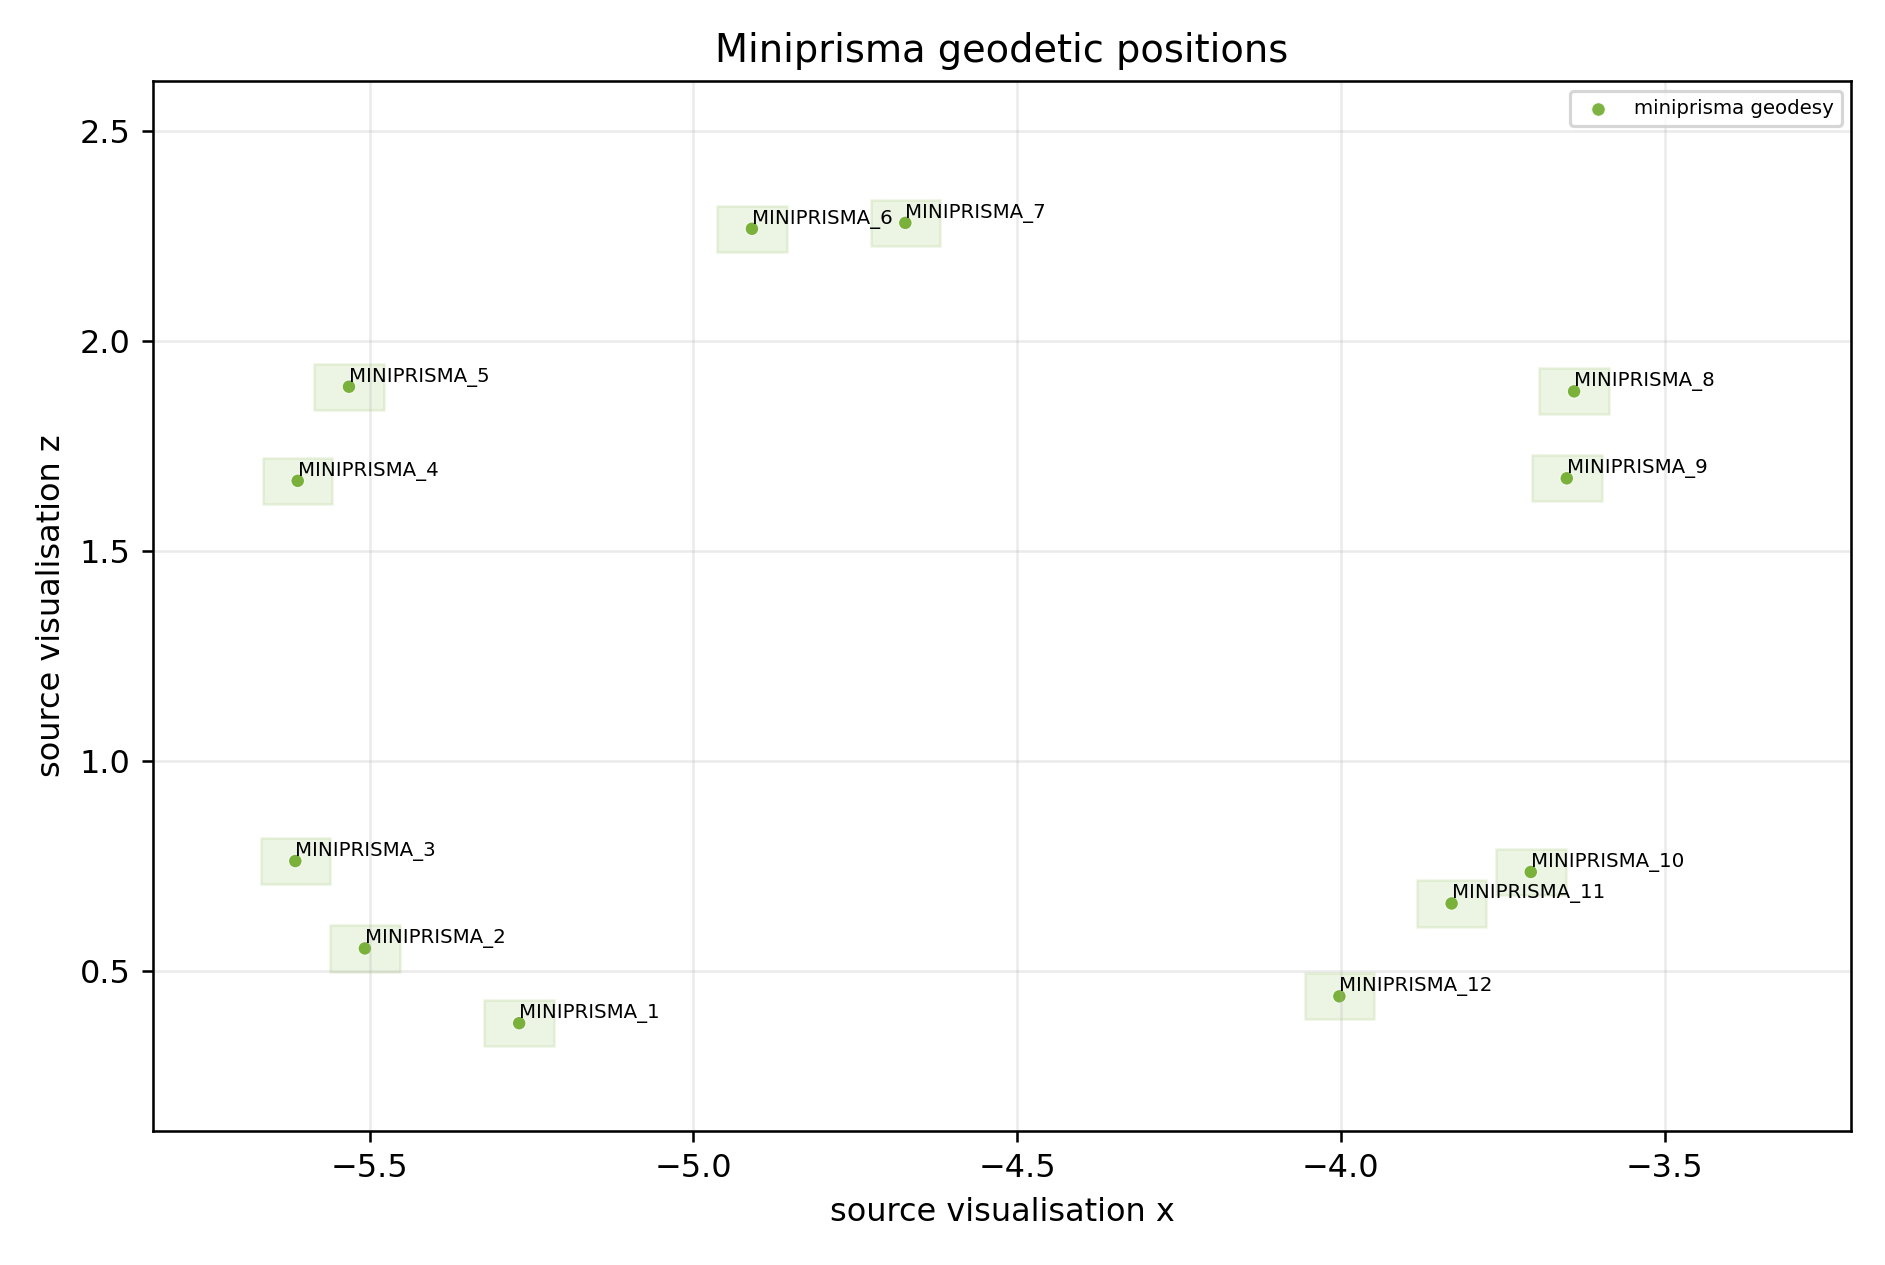
\includegraphics[width=0.95\textwidth]{figures/hm_miniprisma_positions.png}
\caption{Miniprisma positions in the source frame.  Each MINIPRISMA point is plotted
separately.  A hard residual would require campaign displacement vectors, survey
covariance, reference epoch, and a documented 3D-to-2D comparison policy for the
current OGS model.}
\label{fig:hm-miniprisma}
\end{figure}

\begin{figure}[H]
\centering
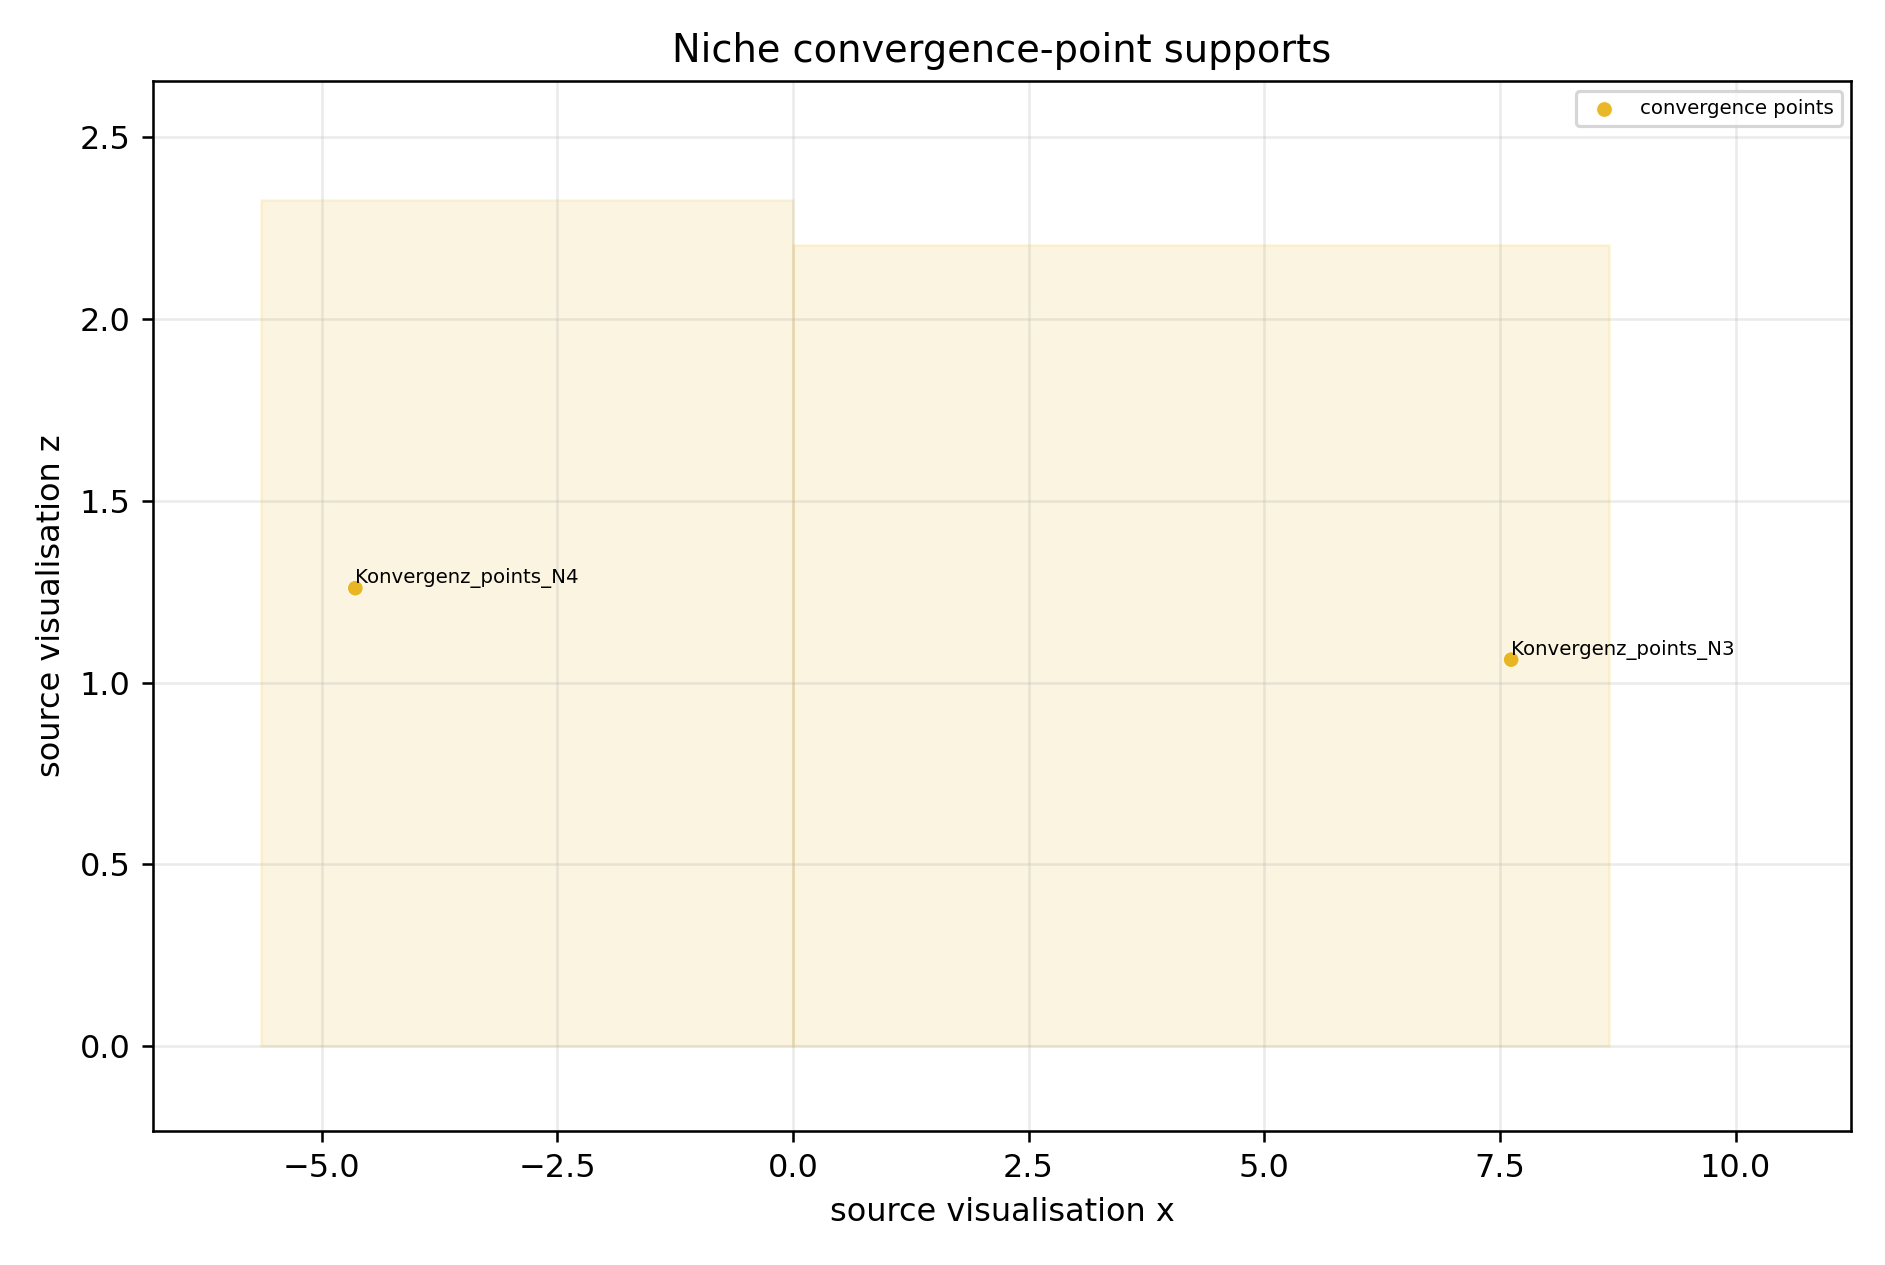
\includegraphics[width=0.95\textwidth]{figures/hm_convergence_positions.png}
\caption{Convergence-point supports in the source frame.  The N3 and N4 convergence
zones would constrain relative displacement of the tunnel or niche contour through
time, but only after the measured convergence series, pair definitions, and reference
epoch are supplied.}
\label{fig:hm-convergence}
\end{figure}

\begin{figure}[H]
\centering
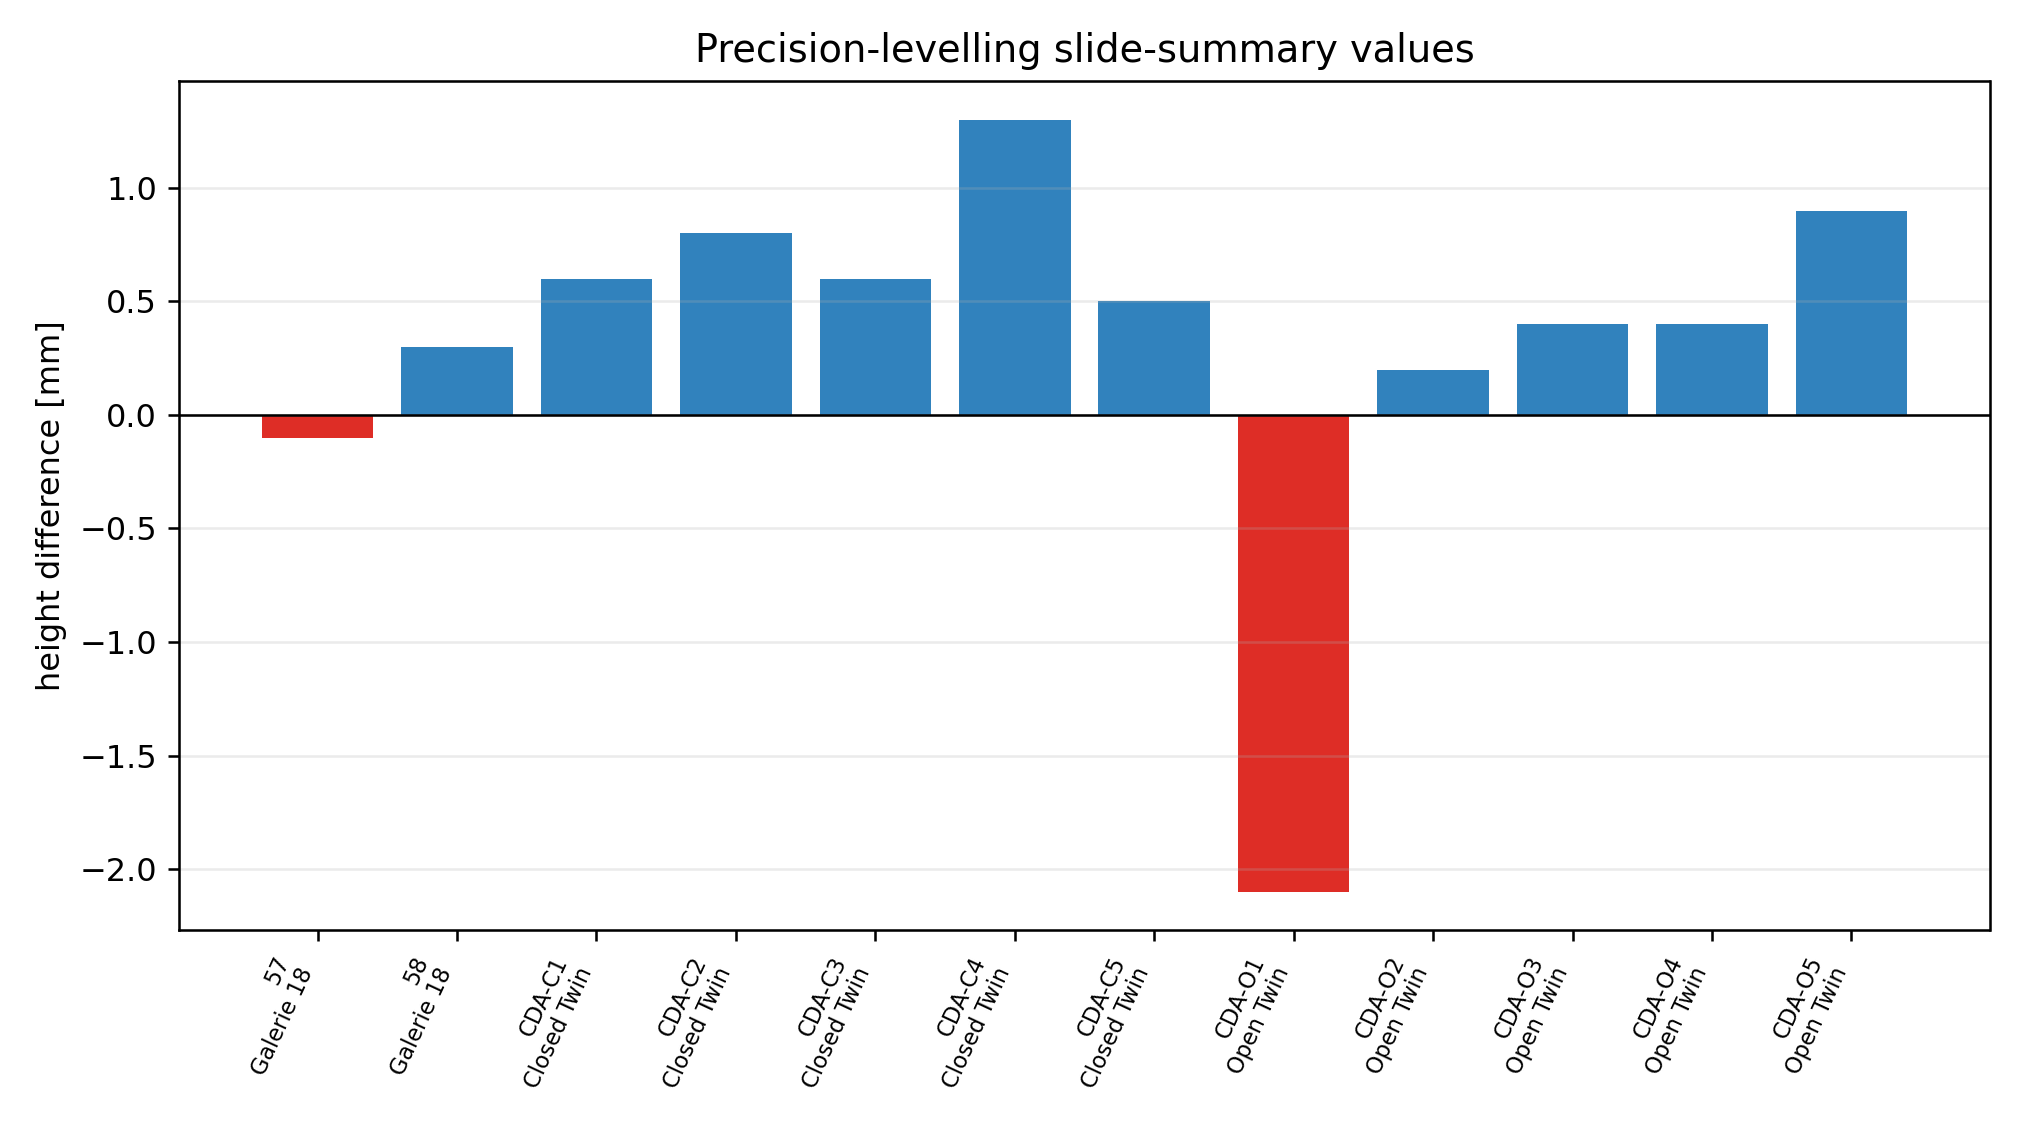
\includegraphics[width=0.98\textwidth]{figures/hm_levelling_values.png}
\caption{Precision-levelling values available from the slide summary.  The values are
height differences between the initial 2022-08-29/30 measurement and the 2026-03
campaign.  They are useful for sign and magnitude checks of vertical displacement,
but the full survey table and covariance are needed before using them as a weighted
mechanical residual.}
\label{fig:hm-levelling}
\end{figure}

\begin{figure}[H]
\centering
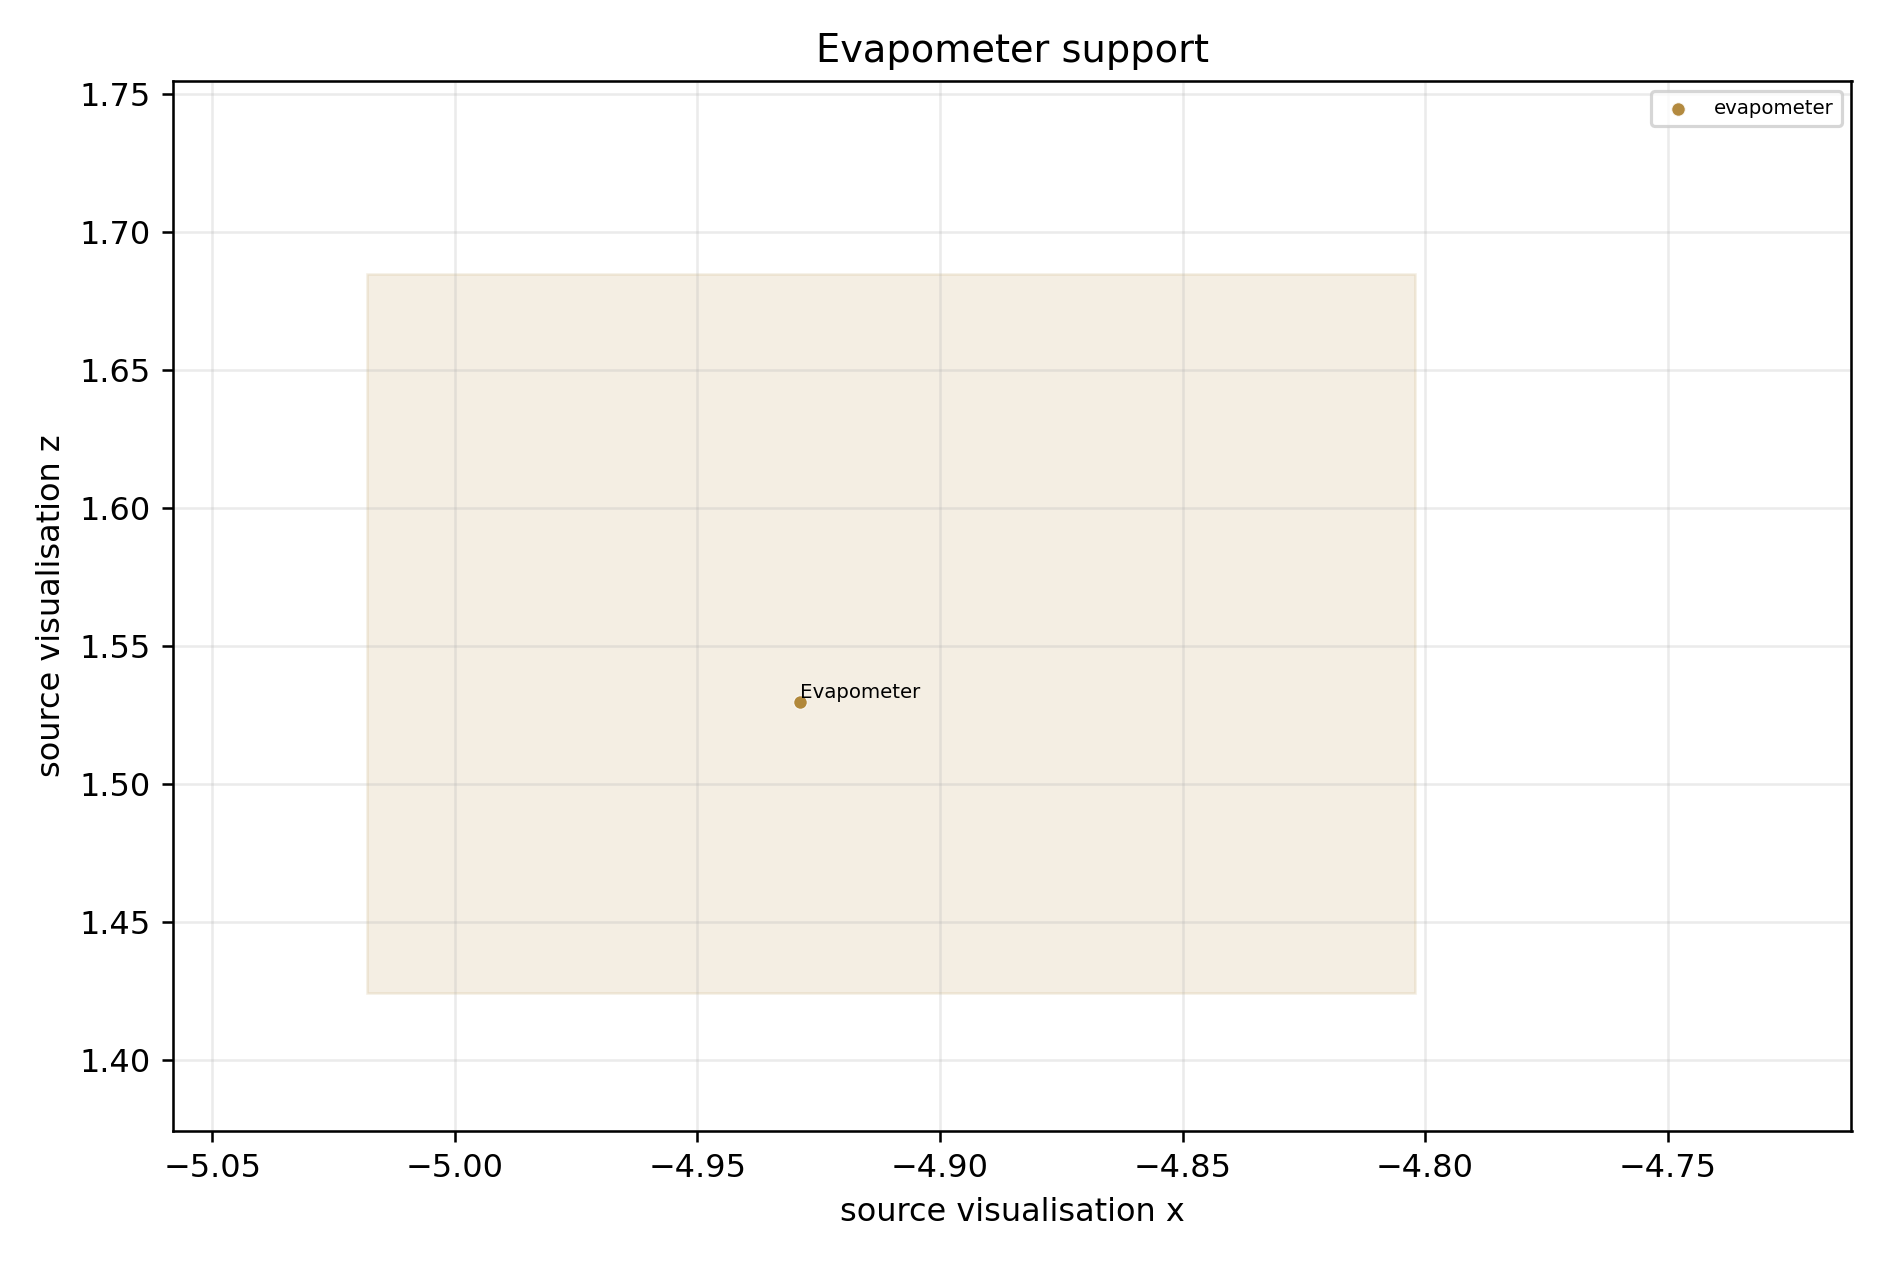
\includegraphics[width=0.82\textwidth]{figures/hm_evapometer_position.png}
\caption{Evapometer support in the source frame.  This is a boundary/climate context
stream for open-niche drying and should only influence inversion through a documented
boundary-flux or boundary-pressure scenario, not as an interior OGS residual.}
\label{fig:hm-evapometer}
\end{figure}

\section{Current Inversion State}

The active field package contains 10,239 positive-definite triangle6 tensor cells,
fixed anisotropy ratio 2.5, bedding angle \(144^\circ\), fixed porosity
\(\npor=0.105\), and current run id
\code{local_basis_sampler_002_basis_024_det_l_0p0075_s_1p000}.  The active objective
components are shown in Figure~\ref{fig:components}.  The field is a legitimate
active-objective incumbent but remains conditional because the field selected by
promoted NMR, accepted ERT, accepted Taupe, or diagnostic rank consensus differs.

\begin{figure}[htbp]
\centering
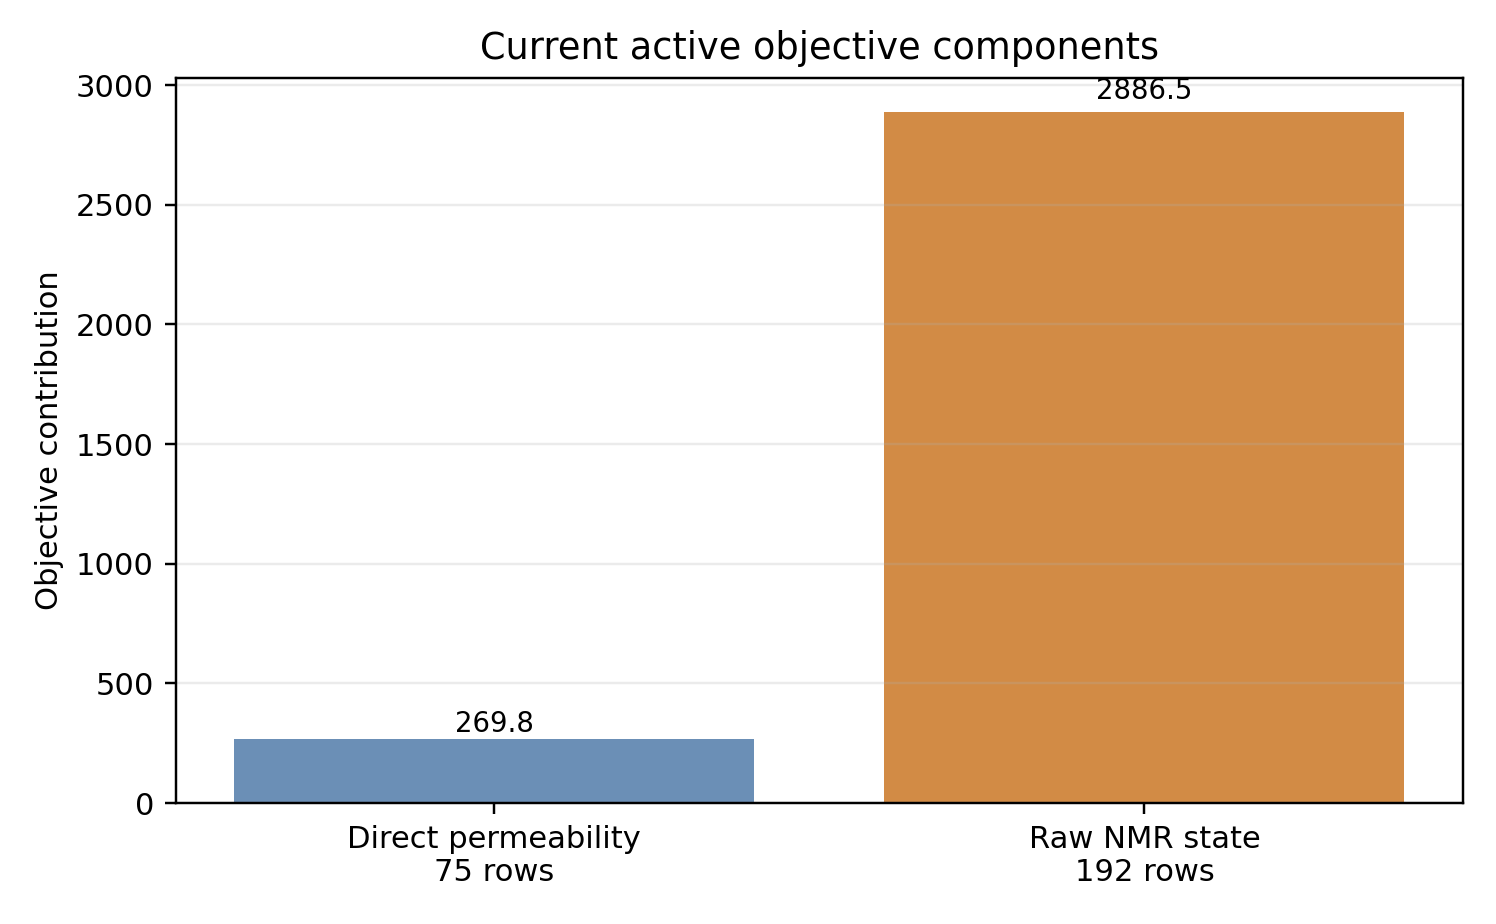
\includegraphics[width=0.68\textwidth]{figures/active_objective_components.png}
\caption{Current active objective components.  The raw NMR term dominates the total
objective, while the direct permeability term is the only direct material-parameter
likelihood.}
\label{fig:components}
\end{figure}

\part*{Annex -- Evidence, Figures, and Audit Findings}
\addcontentsline{toc}{part}{Annex -- Evidence, Figures, and Audit Findings}

\section{Annex A: Source-Data Inventory}

\begin{longtable}{@{}L{0.18\textwidth}L{0.31\textwidth}Y@{}}
\caption{Second-pass mined measurement facts carried into the technical report.}\\
\toprule
Group & Concrete available content & Technical implication \\
\midrule
\endfirsthead
\toprule
Group & Concrete available content & Technical implication \\
\midrule
\endhead
\bottomrule
\endlastfoot
ERT & 15 copied source files; ERT ZIP with 1,736 indexed members, including 1,675 VTK fields and 61 timestep/list files; raw example with 72-electrode open/closed files and \(\code{tx0}\)/\(\code{ohm}\) inputs. & Source depth is strong, but residual activation still needs accepted transform, support, and covariance. \\
NMR & 54 source/data files; 170 weekly rows; 294 seasonal campaign-position rows; seasonal values 2.766--22.810 vol.\%. & Strong near-niche water-content evidence, but total NMR water cannot be equated directly with mobile \(nS_\ell\). \\
Permeability & 6 source files; 204 interpreted interval rows; 6,687 pressure-decay rows. & Direct \(\K\) evidence, but gas pulse tests are noisy interval-scale scalar observations with support conflicts. \\
Taupe/TDR & 10 source files; 5,088 reshaped rows over A3, A4, A7, A8, dates 2019-12-01 to 2025-10-10. & Trend diagnostics are possible; absolute calibration is missing. \\
Suction/RH & 10 source files; 4,247 daily rows; RH5/RH6 near 93--96\%; RH7/RH8 contain low-outlier values near 13\%. & Useful for boundary-curve audit and retention context, not yet a verified replacement forcing. \\
Coordinates/layout & 8 source files; 107 measurement coordinate rows; 35 borehole/endpoint rows. & Essential for all observation operators; some rows lie outside current Niche-4 mesh. \\
Bedding/geology & Bedding image, bedding-page PDF, and characterization-paper copies. & Provides tensor orientation and structural prior, not a direct residual. \\
Other HM & 12 source files including minutes, slides, levelling/HERMES context, and Tecplot layout. & Qualitative/deformation context only until numeric exports and uncertainties arrive. \\
Projection inputs & 87 source files; project/XML/VTU/projection assets and OGS 6.5.4 container material. & Implementation bridge for mesh fields and monthly model outputs; keeps original process semantics frozen. \\
\end{longtable}

\section{Annex B: Permeability Field and Support Diagnostics}

\begin{figure}[p]
\centering
\begin{subfigure}{0.48\textwidth}
\centering
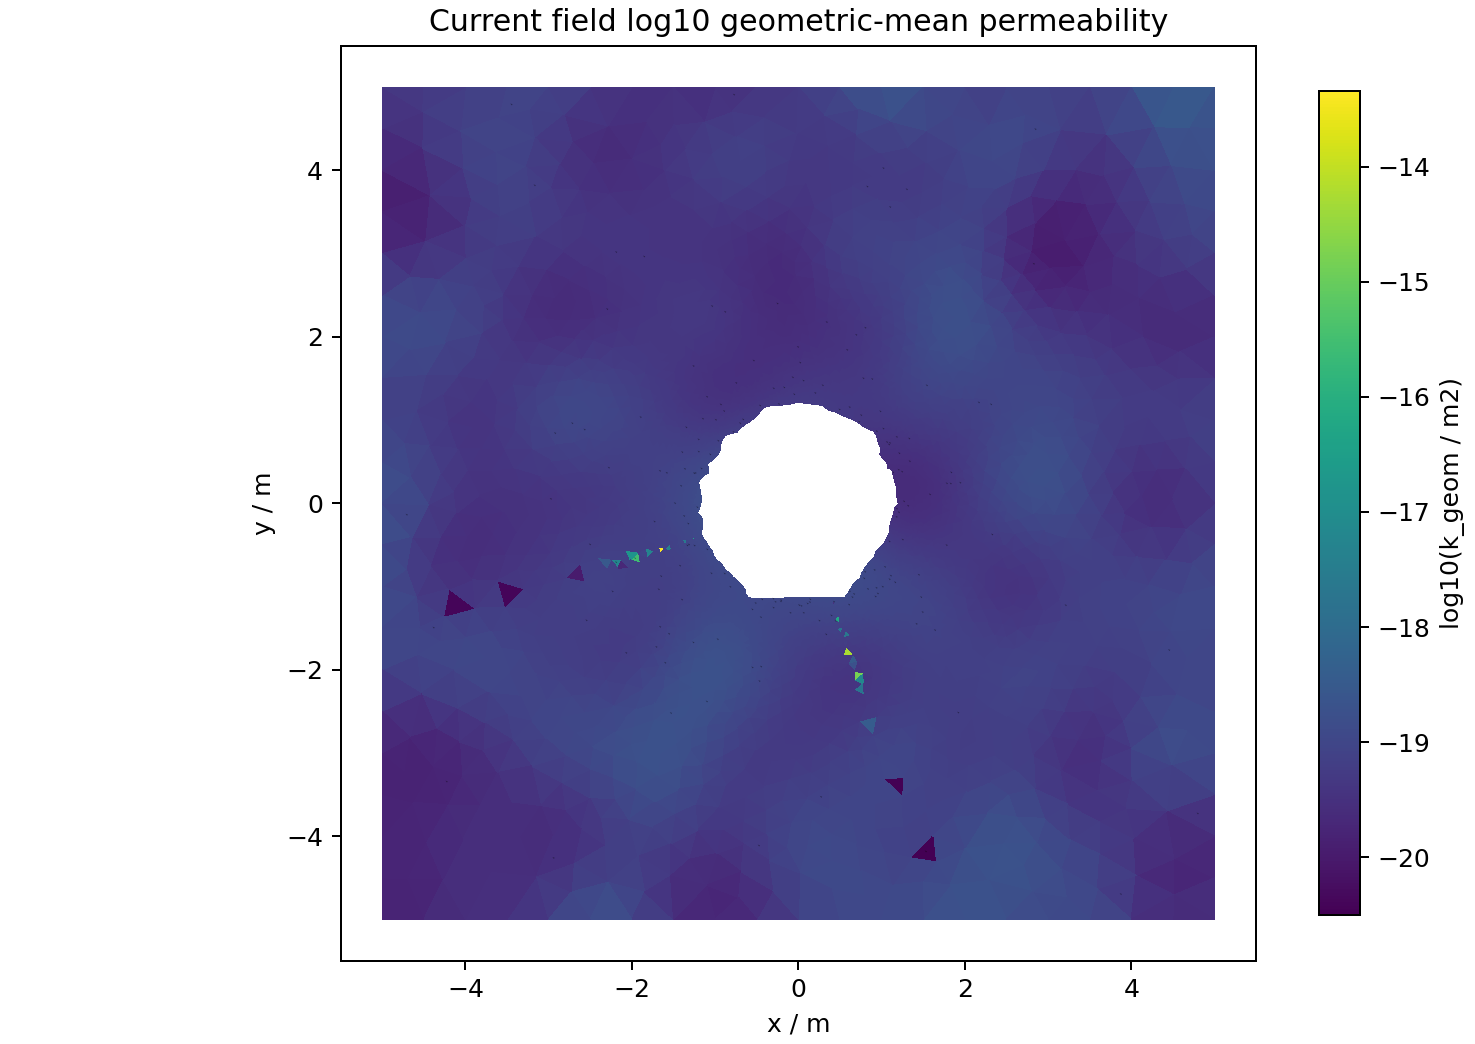
\includegraphics[width=\linewidth]{figures/log10_k_geom_map.png}
\caption{Current log10 geometric-mean permeability map.}
\end{subfigure}
\hfill
\begin{subfigure}{0.48\textwidth}
\centering
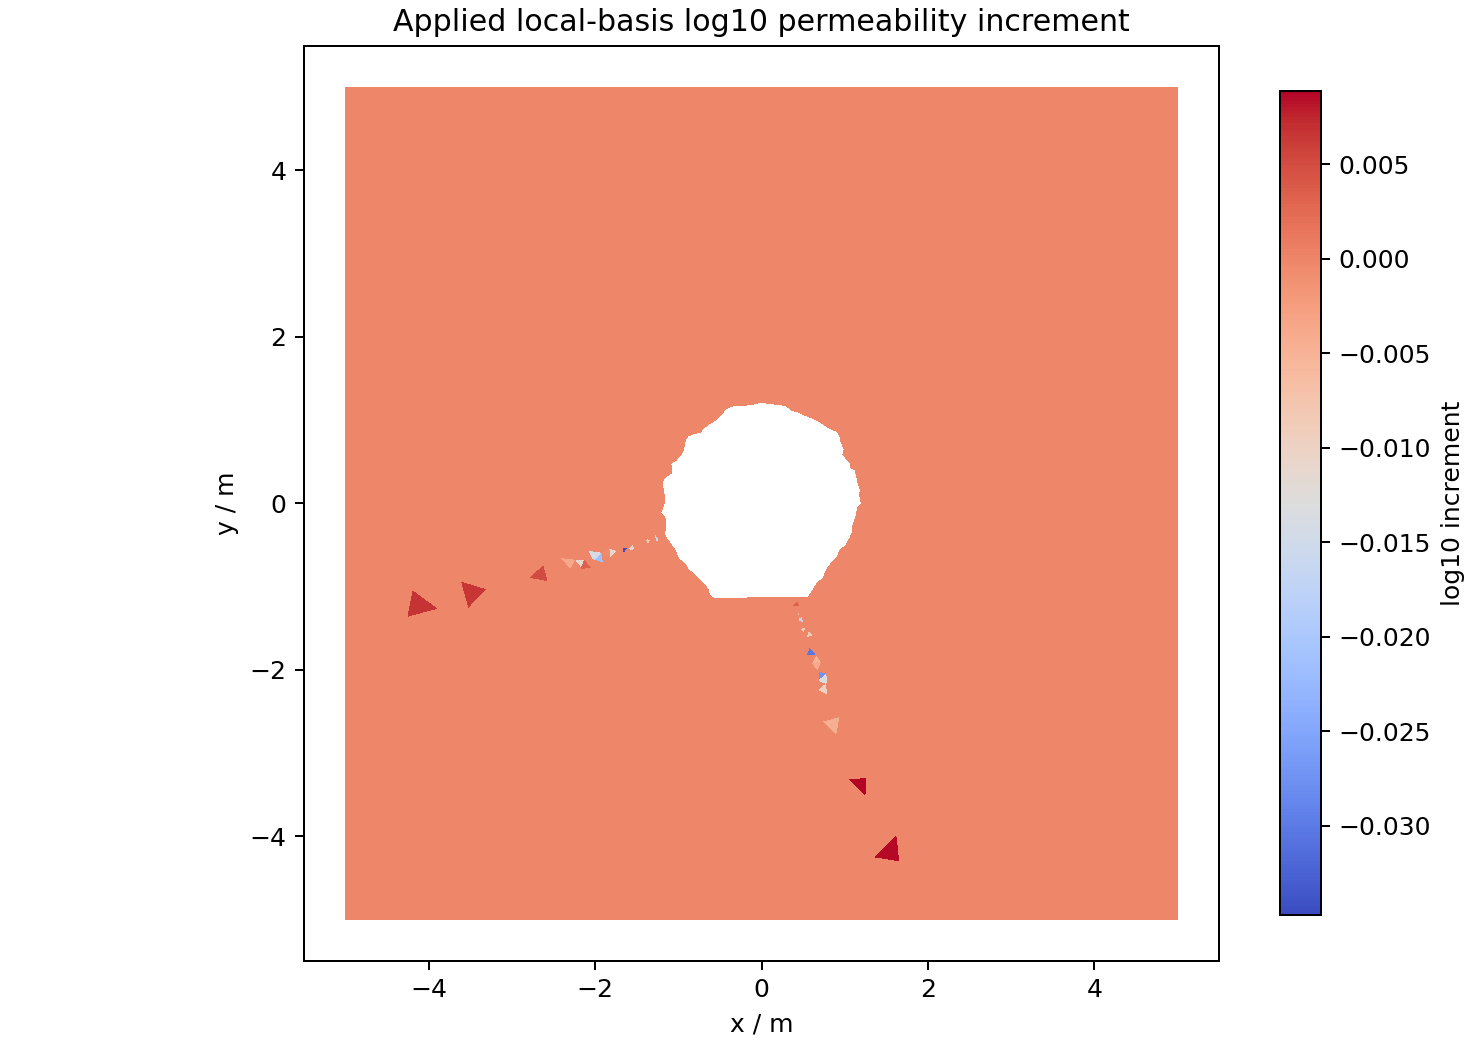
\includegraphics[width=\linewidth]{figures/local_basis_increment_map.png}
\caption{Local-basis log10 increment map.}
\end{subfigure}
\caption{Current active-objective field visual inspection.  The field keeps fixed
anisotropy ratio and angle while applying local magnitude increments around pulse-test
anchors.}
\label{fig:fieldmaps}
\end{figure}

\begin{figure}[p]
\centering
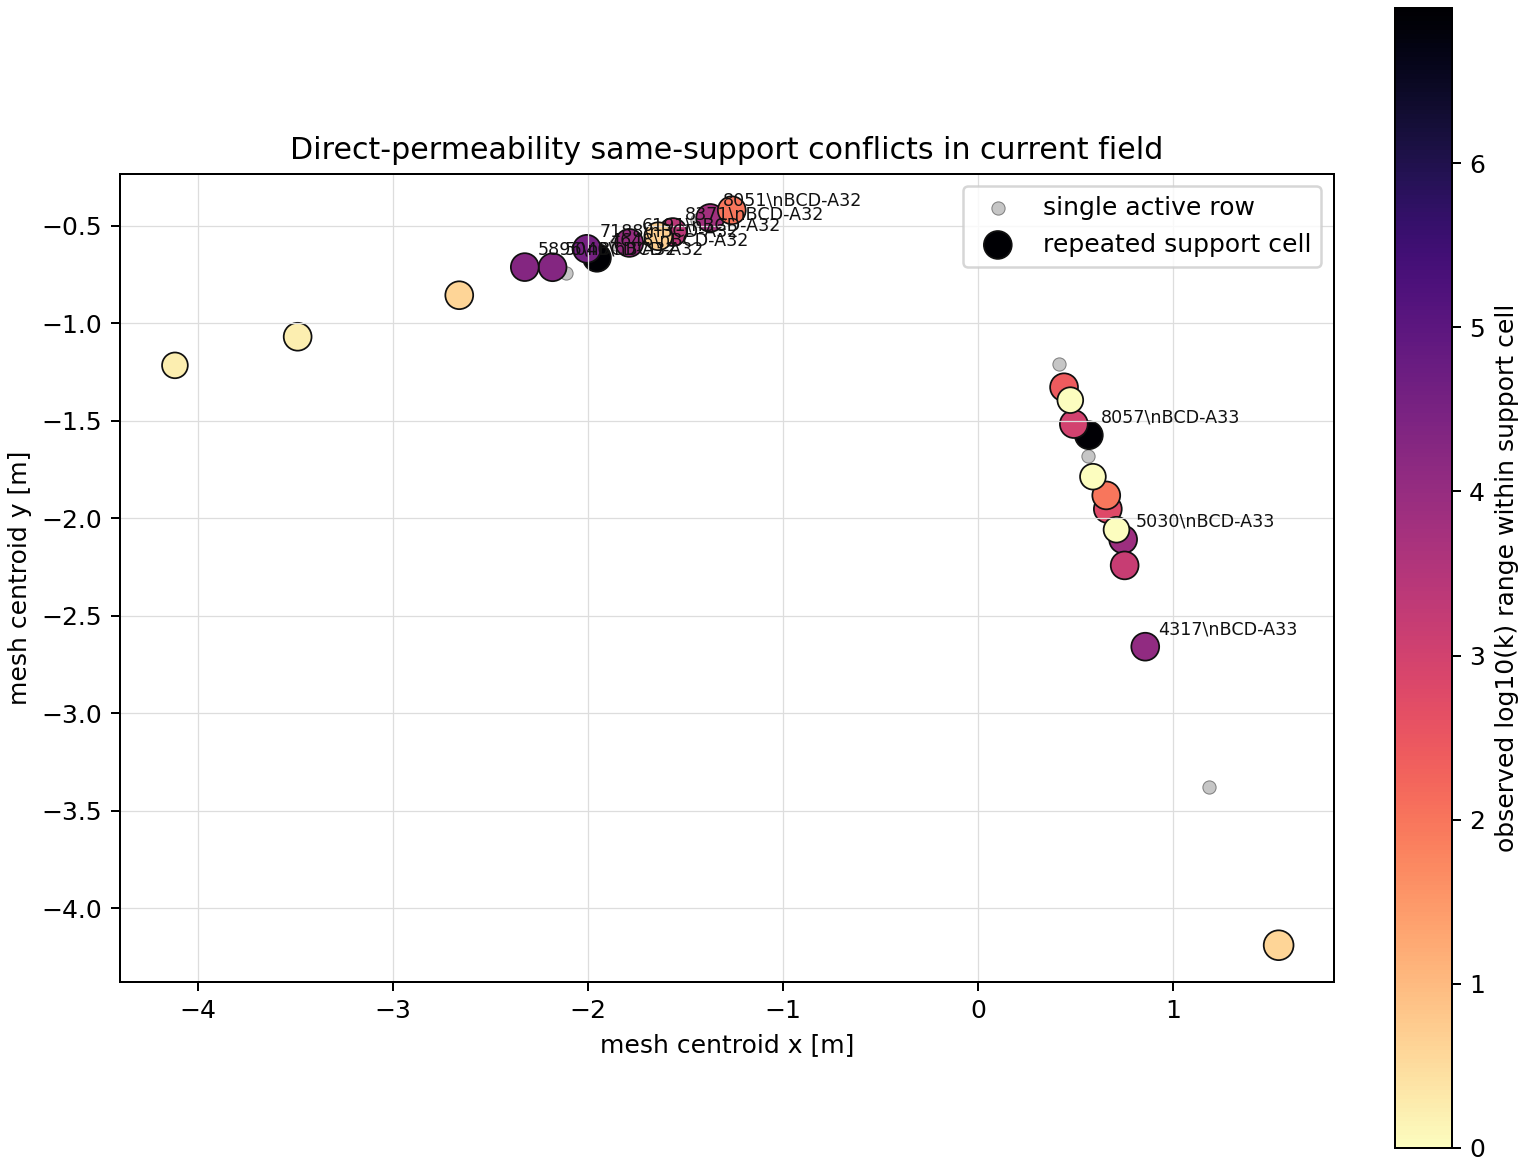
\includegraphics[width=0.88\textwidth]{figures/permeability_support_conflict_spatial_audit.png}
\caption{Spatial support-conflict audit for direct permeability rows.  The same
support cells can carry multiple interpreted pulse-test rows with large log10 spread,
which is why direct permeability likelihood/support policy still needs explicit
acceptance.}
\label{fig:supportconflict}
\end{figure}

\begin{longtable}{@{}L{0.26\textwidth}L{0.18\textwidth}Y@{}}
\caption{Current field statistics relevant to stochastic interpretation.}\\
\toprule
Quantity & Current value & Interpretation \\
\midrule
\endfirsthead
\toprule
Quantity & Current value & Interpretation \\
\midrule
\endhead
\bottomrule
\endlastfoot
Cells & 10,239 triangle6 cells & All are positive definite in the current package. \\
\(\log_{10}k_{\min}\) median & \(-19.385\) & Minor eigen-permeability median. \\
\(\log_{10}k_{\max}\) median & \(-18.987\) & Major eigen-permeability median. \\
Anisotropy ratio & 2.5 everywhere & Tensor shape fixed; magnitude field varies. \\
Tensor angle & \(144^\circ\) everywhere & Bedding-informed orientation. \\
Porosity & 0.105 everywhere & Fixed support field, not active porosity inversion. \\
Direct residual RMSE & 1.611 log10 units & Broad residual remains because active pulse-test rows conflict at support scale. \\
Raw NMR normalized RMSE & 5.483 & Raw absolute NMR residual remains semantically caveated. \\
\end{longtable}

\section{Annex C: Cross-Stream Candidate Evidence}

\begin{figure}[p]
\centering
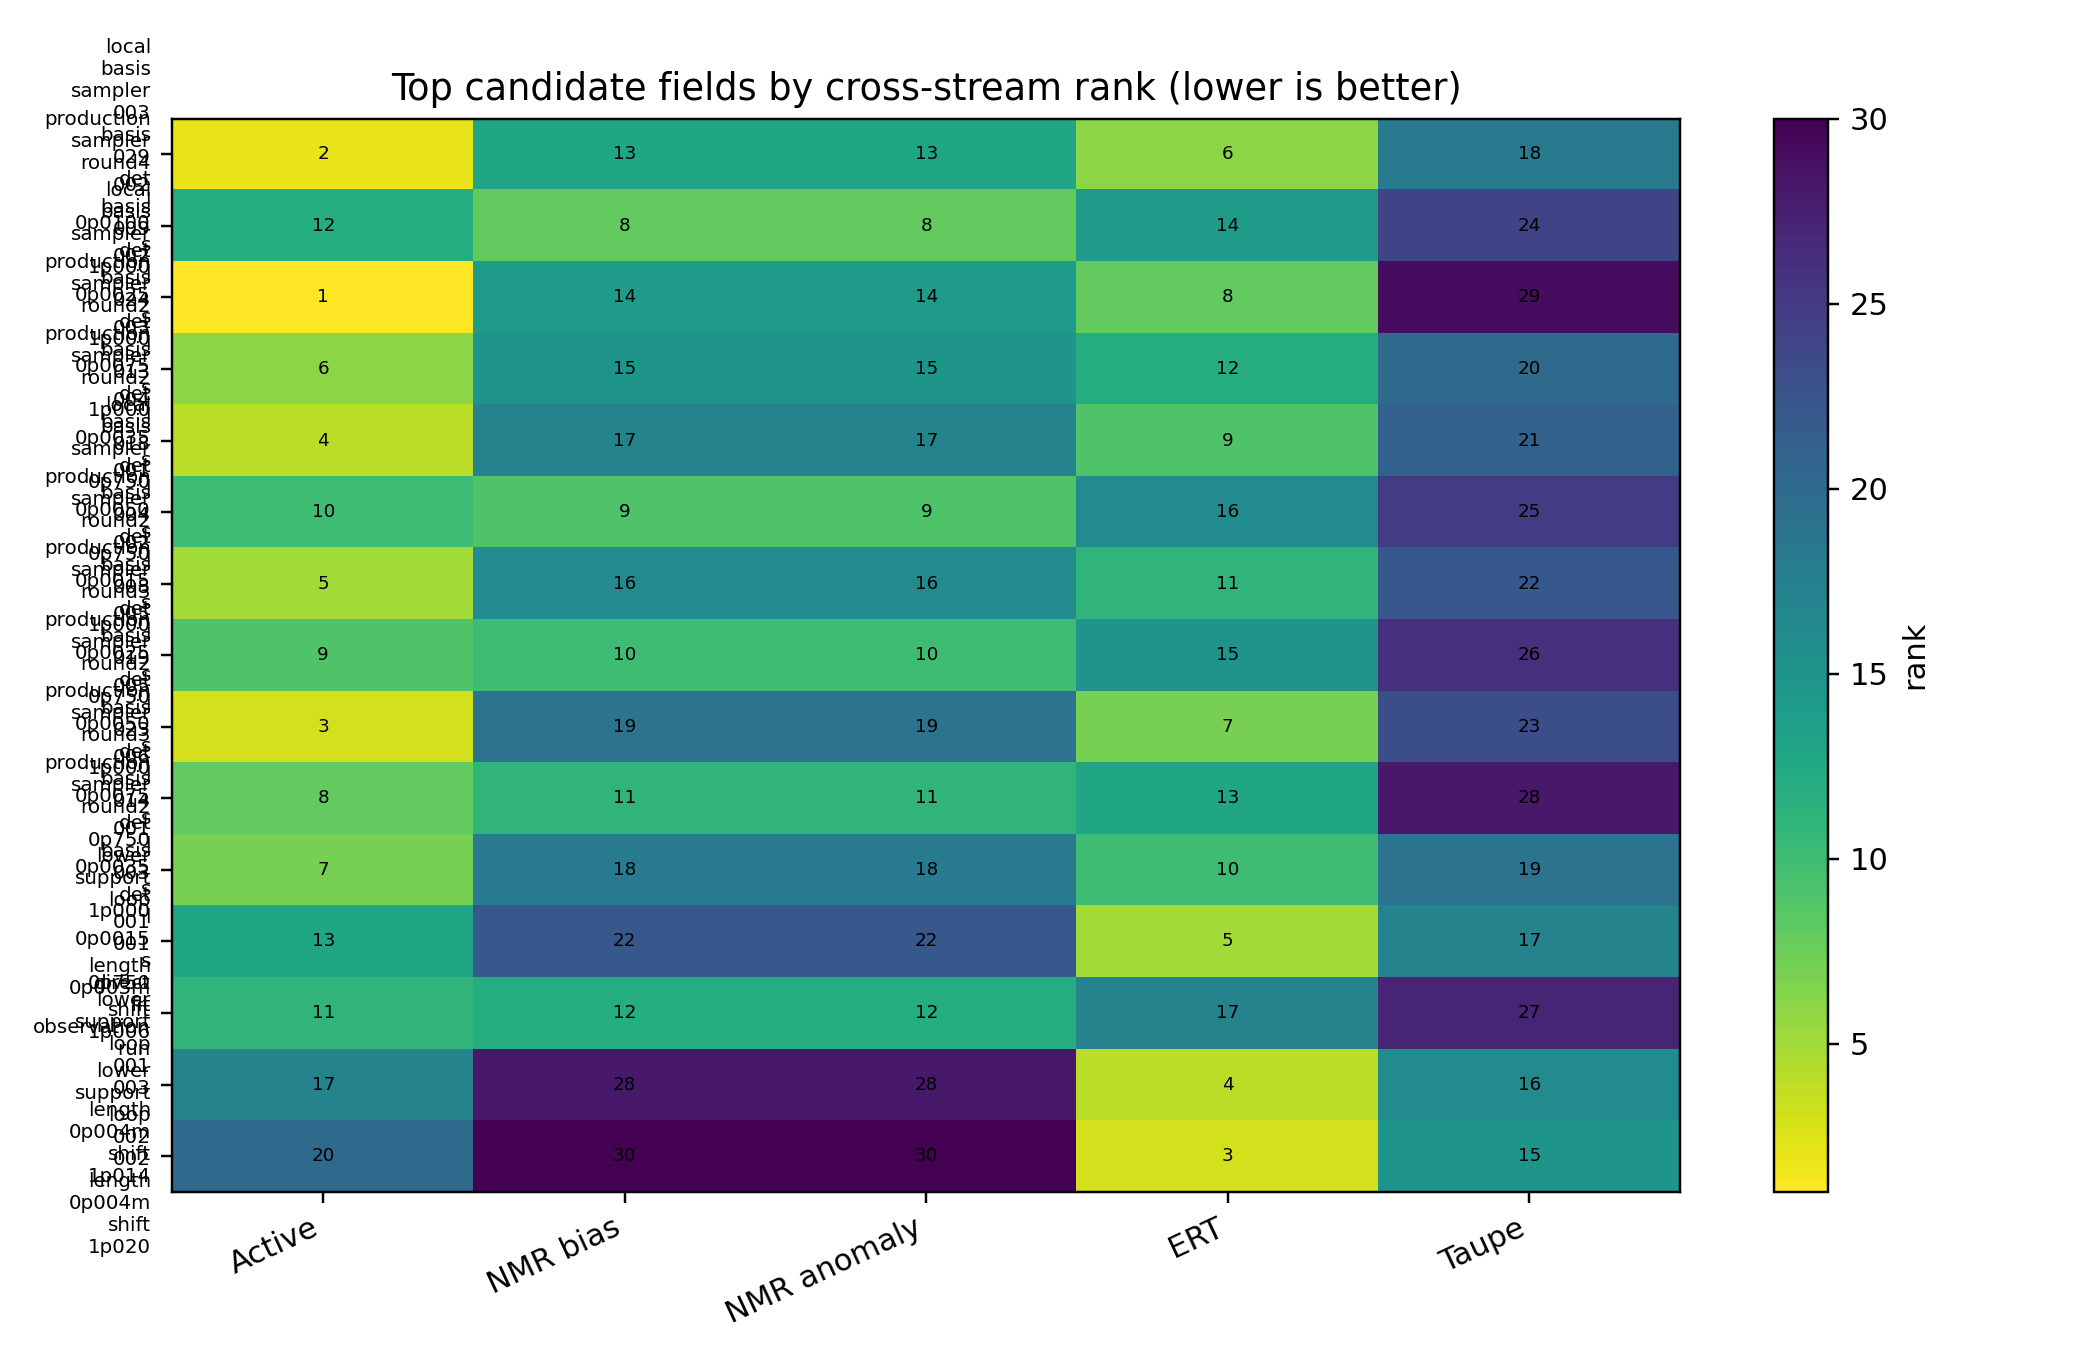
\includegraphics[width=\textwidth]{figures/cross_stream_rank_heatmap.png}
\caption{Top candidate fields by cross-stream rank.  Lower rank is better.  The
active-objective incumbent is not the best mean-rank compromise, and no candidate is
top-10 in every stream.}
\label{fig:rankheatmap}
\end{figure}

\begin{figure}[p]
\centering
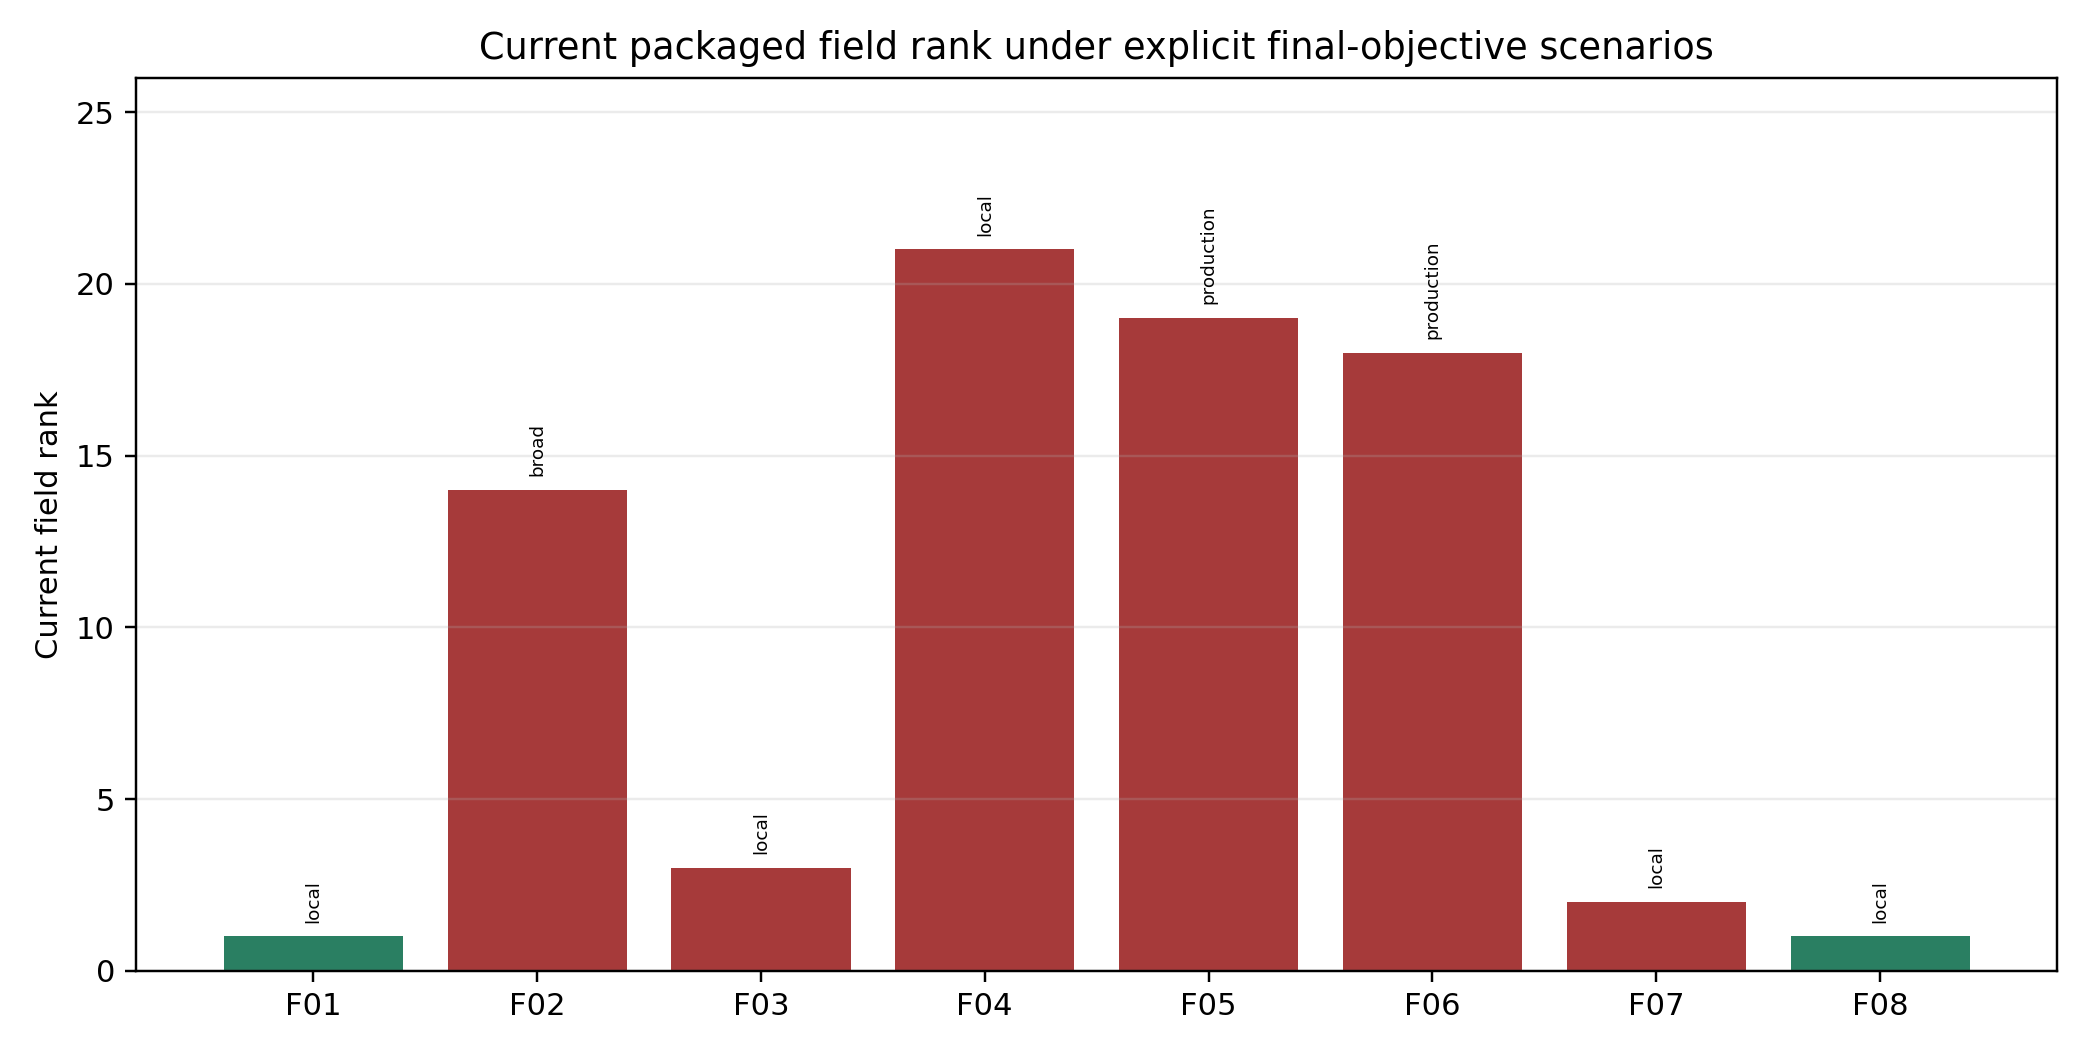
\includegraphics[width=0.86\textwidth]{figures/scenario_current_rank.png}
\caption{Current packaged-field rank under explicit final-objective scenarios.  The
current field wins only the current raw-NMR active objective and the direct-only
tie case; accepted/promoted diagnostic streams select different winners.}
\label{fig:scenariorank}
\end{figure}

\begin{longtable}{@{}L{0.2\textwidth}L{0.21\textwidth}L{0.16\textwidth}Y@{}}
\caption{Final-objective scenario consequences.}\\
\toprule
Scenario & Winner & Current rank & Meaning \\
\midrule
\endfirsthead
\toprule
Scenario & Winner & Current rank & Meaning \\
\midrule
\endhead
\bottomrule
\endlastfoot
Current raw-NMR active objective, gated streams excluded & Current packaged field & 1 & The field is valid only under explicit exclusions/diagnostic-only decisions. \\
Promoted NMR trend/anomaly & Broad continuous 001-003, \(0.021\) m & 14 & NMR free-water policy changes the selected field. \\
Raw NMR plus accepted ERT screen & Local basis 003, basis 029 & 3 & Current field is close but not the scenario winner. \\
Raw NMR plus accepted Taupe screen & Local bracketed 003, \(0.031\) m & 21 & Taupe trends prefer a broader smooth-family candidate. \\
Raw NMR plus accepted ERT and Taupe & Production round 3, candidate 002 & 19 & Combined diagnostics change the field family. \\
Promoted NMR plus accepted ERT and Taupe & Production round 3, candidate 002 & 18 & Closest scored all-numeric scenario still excludes RH, other-HM, and endpoint rows. \\
Diagnostic rank consensus & Local basis 003, basis 029 & 2 & Not a likelihood unless an explicit waiver is accepted. \\
Direct permeability only & Current packaged field, tie & 1 & Direct-only selection has 12 tied best fields; a tie-break policy is missing. \\
Wait for RH/other-HM/endpoint expansion & Not scored & n/a & Requires new provider data and rebuilt scenarios. \\
\end{longtable}

\section{Annex D: Open Gates and Required Decisions}

\begin{longtable}{@{}L{0.24\textwidth}L{0.16\textwidth}Y@{}}
\caption{Blocking items that prevent a final all-measurement field claim.}\\
\toprule
Gate & Priority & What must be supplied or decided \\
\midrule
\endfirsthead
\toprule
Gate & Priority & What must be supplied or decided \\
\midrule
\endhead
\bottomrule
\endlastfoot
ERT transform and support & High & Confirm coordinate origin/axes/units, ERT-to-OGS transform, exact tunnel/niche support mask, and 35 cm rock-depth handling. \\
ERT uncertainty/covariance & High & Provide sigma/correlation/aggregation rule so dense VTK pixels are not treated as independent rows. \\
Taupe/TDR unit and calibration & High & Define workbook units, calibration equations, baseline, sensor/band uncertainty, and whether values are water content, permittivity, or proxy. \\
RH active boundary curve provenance & High & Provide source table/script, sensor screening, time zero, Kelvin constants, smoothing, extension policy, and open/closed mapping. \\
Other-HM numeric exports & High & Provide Geoscope, laser-scan statistical products, levelling tables, extensometer/crackmeter series, and uncertainty metadata. \\
Historical permeability endpoints & Medium & Provide endpoint coordinates/traces for BCD-A24, BCD-A25, BCD-A26, BCD-A27, and BFM-D19 if older rows should enter the fit. \\
NMR final residual policy & High & Choose raw absolute theta with caveats, within-label trend/anomaly, label-bias correction, or exclusion. \\
Direct permeability support policy & High & Decide row-wise Gaussian, robust likelihood, support-cell aggregation, configured outliers, or new field family before more same-support fitting. \\
CTE value/provenance & High & Confirm whether \(\code{CTE}=1254.74\) is intended, inactive, a typo, or copied from heat capacity. \\
\end{longtable}

\section{Annex E: Practical Interpretation}

The safest current scientific wording is:

\begin{quote}
The current CD-A OGS inversion state supports an active-objective permeability field
conditioned on direct gas-pulse permeability rows and raw NMR water-content residuals.
It does not yet support a final all-measurement heterogeneous permeability field.
Permeability heterogeneity is physically and statistically justified as a stage-1
unknown, but porosity, retention, tensor shape, mechanical, thermal, and boundary
parameters should remain fixed or scenario-only until the listed measurement gates
are closed or explicitly excluded.
\end{quote}

The available data do support further heterogeneous modelling, but not arbitrary
heterogeneity.  The strongest near-term route is to keep the PDE/OGS process frozen,
continue using mesh-cell permeability fields, and bring ERT, Taupe/TDR, RH, and HM
streams into the objective only after their observation operators and uncertainty
models are accepted.  Any claim stronger than that would depend on unresolved
provider data or internal policy decisions.

\bibliographystyle{abbrvnat}
\bibliography{references}

\end{document}
